\chapter{Higgs Plus Jets with Finite Quark Mass Effects}

%Chapter about work on getting the impact factor in $qg \to qgH$ relaxing our assumption that the Higgs is far from the gluon in rapidity and keeping the full dependence on the top mass. Focus on how the HE and infinite top mass limits commute, so this is `simple' to include. Also include interference with bottom quark loops. References to \cite{Duca2003}, \cite{DelDuca2001}, \cite{Hahn1999}. Approximately 40\% done, since the document describing how the amplitude is derived is still being written. 

It was briefly discussed that the addition of particles not charged under QCD such as the $W^\pm$, $Z$ and Higgs bosons are included in HEJ by deriving an expression for the emission of the boson that does not interfere with the general factorisation process. In this chapter, we look more closely at how this is done for the case of the Higgs boson (or simply `$H$') in a collection of limits. We will begin with the limit where the Higgs boson is emitted far apart from all other partons in rapidity and where the top quark mass is taken to infinity (the `infinite top mass limit'). Then we will relax the rapidity assumption on the Higgs and allow it to be produced close to an extremal parton in rapidity. Once this is established, we will consider the same rapidity situations but where we no longer use the infinite top mass limit and this will constitute the author's own work. By the end of the chapter, we will have an expression that allows for the Leading Log resummation of Higgs plus at least two jets processes with full quark mass dependence, a calculation that is unique to HEJ.   
\todo{Add new reference for bottom mass}
\section{The Infinite Top Mass Limit}
%HEJ `doesn't care' about whether the infinite top mass limit is implemented or not, so keeping full generality is `easy'. Discussion of why interference effects between top/bottom quark loops might be important (see, for example, \cite{Grazzini2013}).
%\todo{Also mention that it is important to describe tails correctly because of VBF cuts}

If we wish to place a Higgs along our rapidity chain which consists of $t$-channel gluon exchanges, then it stands to reason that we need to couple the Higgs to the gluon in some fashion. However, the Higgs coupling to the gluon is zero because the latter is a massless particle. Generally, what we need to do is couple the Higgs to a quark loop (the top loop is the most dominant, since the coupling depends on the mass of the particle that the Higgs is coupling to) which connects to the gluons in the chain. Loops generally complicate the calculation of an amplitude and thus even the calculation to leading order for this case is more involved than a pure QCD process. This will be demonstrated further in the later sections of this chapter. In order to get around this complication, theorists and phenomenologists sometimes take the limit where the top mass tends to infinity. This effectively `shrinks' the quark loop to a point and so we end up with an \emph{effective} gluon-gluon-Higgs coupling in our Lagrangian\footnote{There is also a gluon-gluon-Higgs-Higgs interaction, but this thesis only concerns itself with single Higgs production and so we leave it out for brevity here.};

\begin{equation}
\mathscr{L}_{QCD + ggH} = \mathscr{L}_{QCD} + \frac{A}{4} G^{\mu \nu}G_{\mu \nu}H,
\end{equation}

with $A = \frac{\alpha_s}{3 \pi v}$ \cite{Duca2003}, resulting in the following Feynman rule for the effective $ggH$ vertex \cite{Andersen2009a};

\begin{equation}
V_H^{\mu \nu}(q_1, q_2) = A \left( \eta^{\mu \nu} q_1 \cdot q_2 - q_1^\nu q_2^\mu \right),
\end{equation}

where $q_1$ is incoming to the vertex and $q_2$ outgoing. Since the Higgs does not carry colour information, we can simply insert this vertex into our FKL amplitude expression so long as the Higgs is far away from all other particles in rapidity. We encode this by first defining the spinor/Lorentz string;

\begin{equation}
S_{qQ \to qHQ}(q_1, q_2) = \matel{1}{\mu}{a} (\eta^{\mu \nu}q_1 \cdot q_2 - q_1^\nu q_2^\mu)\matel{2}{\nu}{b}. 
\end{equation} %I am sure of the 3 pi v here

With this, we can express the $qQ \to qHQ$ helicity and colour summed and averaged square of the amplitude as;

\begin{equation}
\begin{split}
|M_{qQ \to qHQ}^{HE,ggH}|^2 &= \frac{1}{4(N_C^2 - 1)} ||S_{qQ \to qHQ}(q_1, q_2)||^2 \\
& \cdot \left(g^2 C_F \frac{1}{\hat{t}_1} \right) \\
& \cdot \left(\frac{1}{\hat{t}_1} \left(\frac{\alpha_s}{3 \pi v} \right)^2 \frac{1}{\hat{t}_2} \right) \\
& \cdot \left(g^2 C_F \frac{1}{\hat{t}_2} \right).
\end{split}
\end{equation}

The generalisation to multiple gluon emissions and different initial states follows as before by colour factor multiplciations and additions of Lipatov vertices, though care is needed to keep track of which $t$-channel momenta are flowing into the Higgs vertex and which are flowing into Lipatov vertices. If instead the Higgs is emitted close to an extremal parton, then this decomposition is no longer valid and we have to include the contributions in some other fashion. Such contributions are included via the use of impact factors \cite{Duca2003}, which are strict high energy expressions that encapsulate this effect.  

The infinite top mass limit is remarkably successful for predictions of inclusive variables like total cross sections. The reason for this is that the expansion of this effective coupling is a power series in $\frac{m_H^2}{4 m_t^2} \sim 0.13$ and we essentially assume the top mass is the most relevant scale in the problem. It was checked that even the addition of a large dijet invariant mass in the amplitude had little effect \cite{Duca2003}. However, if the transverse scales start to become larger than the top mass (in particular, the transverse scales of the gluons entering the effective vertex), there is significant deviation between the result obtained in the full and effective theories \cite{Duca2003}. \\
\\
For HEJ, the infinite top mass limit was included because the expressions are simpler, but note that the factorisation of amplitudes will still occur whether or not this limit is taken. Therefore, any derived vertices for Higgs production with the full quark mass included can still be implemented in a straightforward way. Furthermore, as soon as the vertex including the full quark mass is derived, we can trivially add in the effect of more than one quark loop (for example, where a bottom quark runs in it). Such interference effects have been shown to produce interesting effects at small $p_T$ scales \cite{Grazzini2013}. For these reasons, we decided to implement the effect of finite quark masses in the HEJ formalism. 

\section{Calculations of $H$ + jets with Finite Quark Mass Effects}

As discussed before, there are two rapidity cases to be discussed; the first where the Higgs is emitted centrally and the second where it is emitted close to an external parton. The base amplitude for the first is the $qQ \to qHQ$ amplitude and for the second it is the $gq \to Hgq$ amplitude. We will begin our discussion with the first case, since it will turn out to be remarkably simple. 

\subsection{$qQ \to qHQ$}

The HEJ expression for the $qQ \to qHQ$ amplitude with full finite quark mass effects is shown diagrammatically in figure \ref{fig:qQh_eff}. In the previous section, we showed how the amplitude was derived in the infinite top mass limit. Because the factorisation properties of the amplitude are unchanged by moving away from this limit, the extension of this amplitude to the full finite quark mass dependent one is found by simply `undoing' the infinite top mass limit on the vertex $V_H^{\mu \nu}$. Such an expression can essentially be looked up, for example in Appendix B of \cite{Duca2003}, so long as care is taken to ensure that incoming and outgoing momenta are labelled correctly. Keeping with the convention before that $q_1$ is incoming and $q_2$ outgoing, the vertex with a finite top mass is;

\begin{equation}
V^{\mu \nu}_{H, m_t}(q_1, q_2) = -\frac{4 g_s^2 m_t^2}{v} \left[\eta^{\mu \nu}A_2(-q_1,q_2) + q_1^\nu q_2^\mu A_1(-q_1,q_2) \right],
\end{equation}

\begin{figure}[t]
\centering
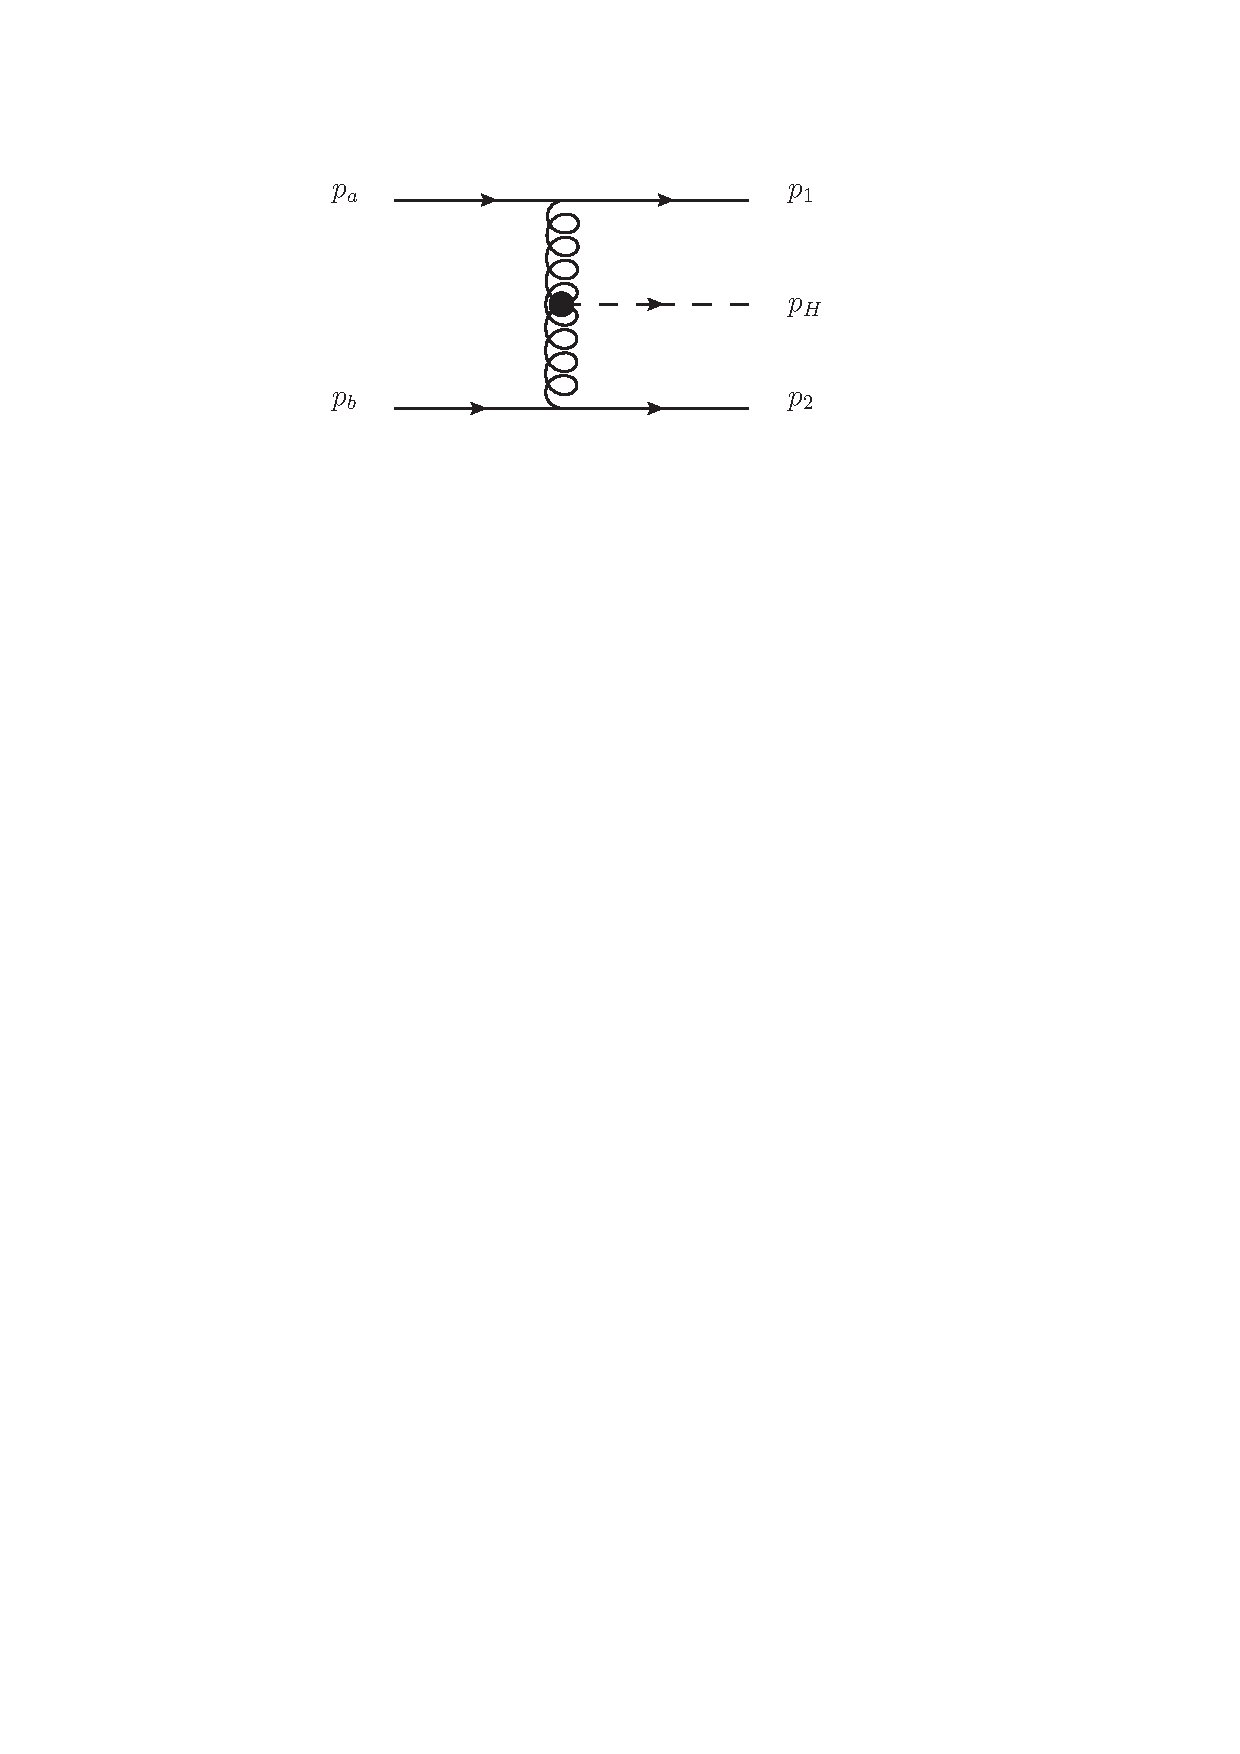
\includegraphics{Images/qQh_eff.pdf}
\caption{Diagrammatic representation of $qQ \to qHQ$ with an effective vertex for the production of the Higgs.}
\label{fig:qQh_eff}
\end{figure}

where $v$ is the Higgs vacuum expectation value ($\approx 246$ GeV) and $A_1, A_2$ depend on a combination of scalar integrals which appear via the integral reduction technique \cite{Tkachov:1981}. We first define \footnote{The integral $B_0$ is actually divergent in 4 dimensions, but will always appear in combinations such that this divergence cancels in later functions.};

\begin{equation}
\begin{split}
B_0(k) &= \int \frac{d^4 q}{(2 \pi)^4} \frac{1}{(q^2-m_t^2)((q+k)^2-m_t^2)}, \\
C_0(p,k) &= \int \frac{d^4 q}{(2 \pi)^4} \frac{1}{(q^2-m_t^2)((q+p)^2-m_t^2)((q+p+k)^2-m_t^2)}, \\
Q &= -q_1 - q_2, \\
\Delta_3 &= (q_1^2)^2 + (q_2^2)^2 + (Q^2)^2 - 2 q_1^2 q_2^2 - 2q_1^2Q^2 - 2q_2^2Q^2,
\end{split}
\label{eqn:scalars}
\end{equation}

which allows us to give the forms of $A_1$ and $A_2$ as;

\begin{equation}
\begin{split}
A_1(-q_1,q_2) &= C_0(-q_1,q_2) \left[\frac{4 m_t^2}{\Delta_3}(Q^2-q_1^2-q_2^2)-1-\frac{4q_1^2q_2^2}{\Delta_3} - \frac{12q_1^2q_2^2Q^2}{\Delta_3^2}(q_1^2+q_2^2-Q^2) \right] \\
&- \left[B_0(q_2)-B_0(Q) \right] \left[\frac{2 q_1^2}{\Delta_3} + \frac{12 q_1^2 q_2^2}{\Delta_3^2}(q_2^2-q_1^2+Q^2) \right] \\
& - \left[B_0(-q_1)-B_0(Q) \right] \left[\frac{2q_1^2}{\Delta_3} + \frac{12 q_1^2 q_2^2}{\Delta_3^2}(q_1^2-q_2^2+Q^2) \right] \\
& - \frac{2}{\Delta_3} \frac{i}{(4 \pi)^2}(q_1^2 + q_2^2 - Q^2) \\
A_2(-q_1,q_2) &=  C_0(-q_1,q_2) \left[2 m_t^2 + \frac{1}{2}(q_1^2+q_2^2-Q^2) + \frac{2 q_1^2 q_2^2Q^2}{\Delta_3} \right] \\
&+ \left[B_0(q_2)-B_0(Q) \right] \frac{1}{\Delta_3}q_2^2(q_2^2-q_1^2-Q^2) \\
& + \left[B_0(-q_1)-B_0(Q) \right] \frac{1}{\Delta_3}q_1^2(q_1^2-q_2^2-Q^2)\\
& +\frac{i}{(4 \pi)^2}.
\label{eqn:afuncs} 
\end{split}
\end{equation}

The scalar integrals can either be evaluated numerically (via, for example, a program like LoopTools \cite{Hahn1999}) or again simply looked up\footnote{It is important to realise that most given results are valid only in certain kinematical regions, so care must be taken to pick the correct analytical formula.} and so the values of $A_1$ and $A_2$ can be worked out at any point. It can be numerically checked that;

\begin{equation}
\begin{split}
\lim_{m_t \to \infty} 4 \frac{g_s^2 m_t^2}{v}A_1(-q_1,q_2) &= i A, \\
\lim_{m_t \to \infty} 4 \frac{g_s^2 m_t^2}{v}A_2(-q_1,q_2) &= -i q_1 \cdot q_2 A, \\
\end{split}
\end{equation}

and thus;

\begin{equation}
\lim_{m_t \to \infty}V^{\mu \nu}_{H, m_t} \to -i V^{\mu \nu}_H,
\end{equation}

where the phase factor of $-i$ arises from a difference in convention and is unimportant since we are always taking the modulus squared of the amplitude. We can therefore simply insert this vertex rather than the infinite top mass vertex into our amplitude to get the result;

\begin{equation}
\begin{split}
|M_{qQ \to qHQ}^{HE,ggH}|^2 &= \frac{1}{4(N_C^2 - 1)} ||S_{qQ \to qHQ}^{\hspace{2pt} m_t}(q_1, q_2)||^2 \\
& \cdot \left(g^2 C_F \frac{1}{\hat{t}_1} \right) \\
& \cdot \left(\frac{1}{\hat{t}_1} \left(\frac{-4 g_s^2 m_t^2}{v} \right)^2 \frac{1}{\hat{t}_2} \right) \\
& \cdot \left(g^2 C_F \frac{1}{\hat{t}_2} \right).
\end{split}
\end{equation}
with;
\begin{equation}
S_{qQ \to qHQ}^{\hspace{2pt} m_t}(q_1, q_2) = \matel{1}{\mu}{a} (\eta^{\mu \nu}A_2(-q_1,q_2) + q_1^\nu q_2^\mu A_1(-q_1,q_2))\matel{2}{\nu}{b}. 
\end{equation}
%\todo{Finish this off with a plot showing the difference}

\subsection{$gq \to Hgq$}

The situation where the Higgs is emitted close to an extremal gluon involves a much more thorough calculation. We will start by finding the general leading order expression and then use knowledge of the high energy limit considered ($y_H \sim y_1 \gg y_2$) to again factorise the expression into the form HEJ requires, which would look diagrammatically like figure \ref{fig:gqH_imp} and mathematically like;

\begin{equation}
M \sim \frac{Z^{\mu}(p_a,p_1,p_H) \matel{2}{\mu}{b}}{\hat{t}_2},
\label{eqn:higgseff}
\end{equation}

\begin{figure}[t]
\centering
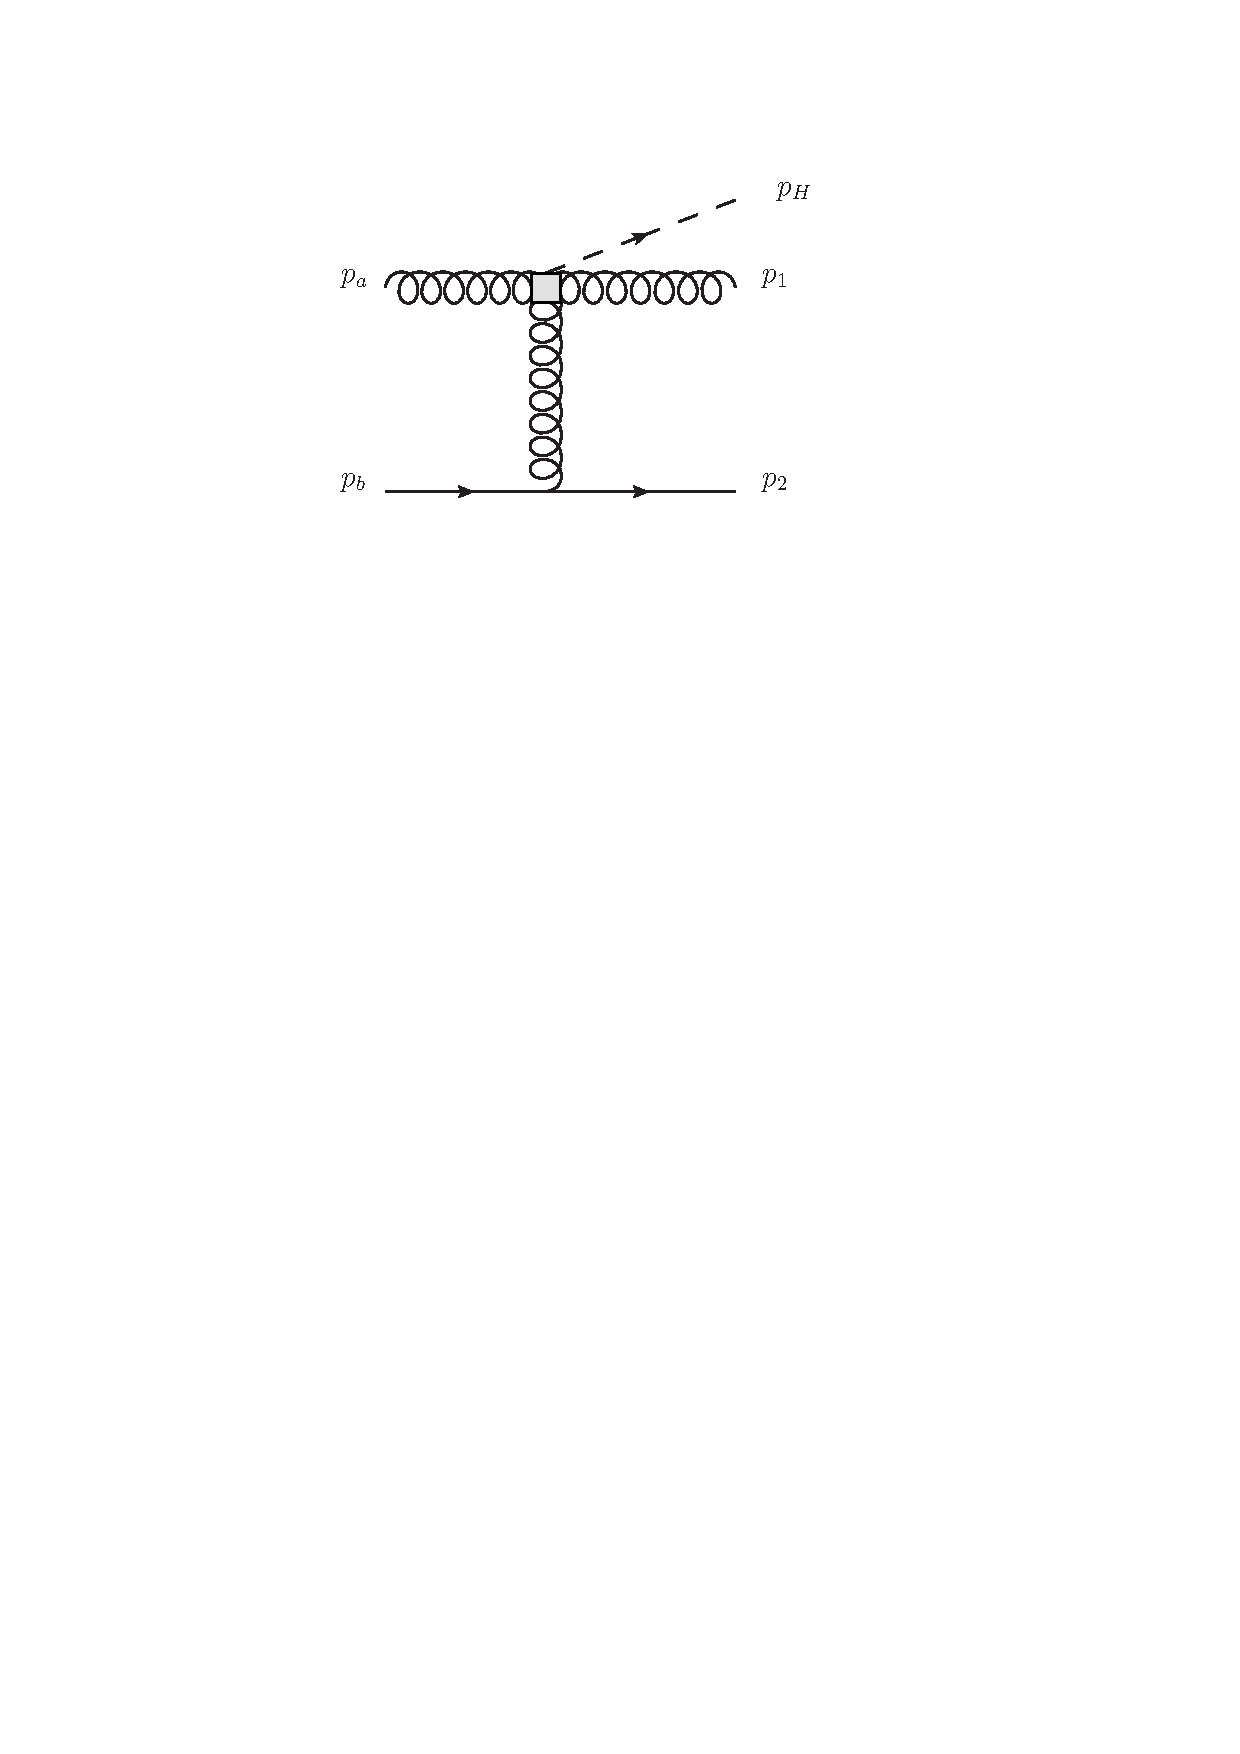
\includegraphics{Images/qgh_impact_factor.pdf}
\caption{Diagrammatical representation of factorised $gq \to gHq$ expression.}
\label{fig:gqH_imp}
\end{figure}

assuming that the polarisation vectors of the external gluons have been contracted with the effective vertex. There are 20 leading order diagrams to consider in total, which is reduced to 10 after invoking Furry's Theorem which states that diagrams involving an anti-quark loop can be related to diagrams with a quark loop. A selection of these diagrams is shown in figure \ref{fig:qgh_lo}. We will use \cite{DelDuca2001} as a guide for our work. In particular, we choose to use the following function for our parametrisation of the top-quark triangle loop, keeping full top mass dependence;

\begin{equation}
T^{\mu_1 \mu_2} = F_T(q_1^2, q_2^2,(q_1+q_2)^2) T_T^{\mu_1 \mu_2} + F_L(q_1^2, q_2^2,(q_1+q_2)^2) T_L^{\mu_1 \mu_2},
\end{equation}

\begin{figure}[t] 
\centering
\subfloat{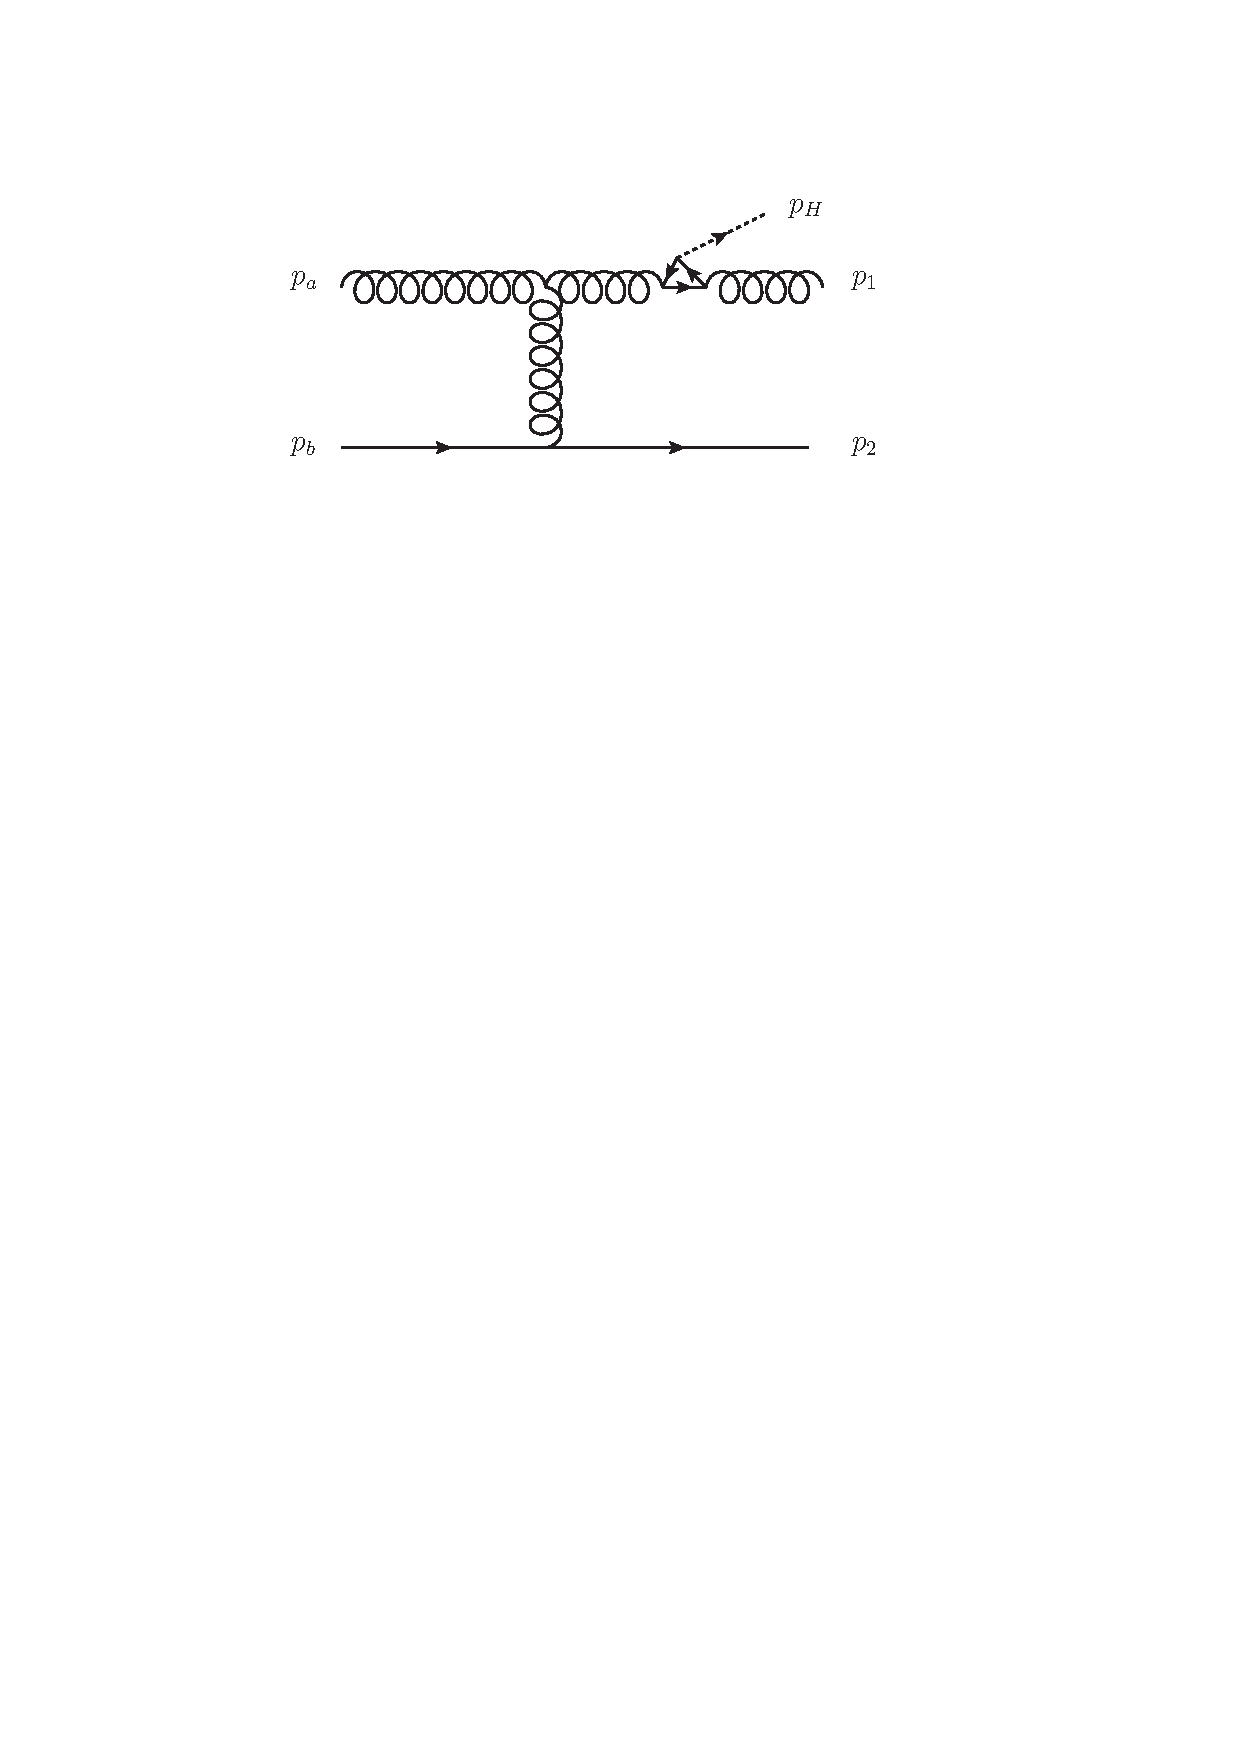
\includegraphics[scale=0.75]{Images/qgh_pa_t.pdf}} 
\subfloat{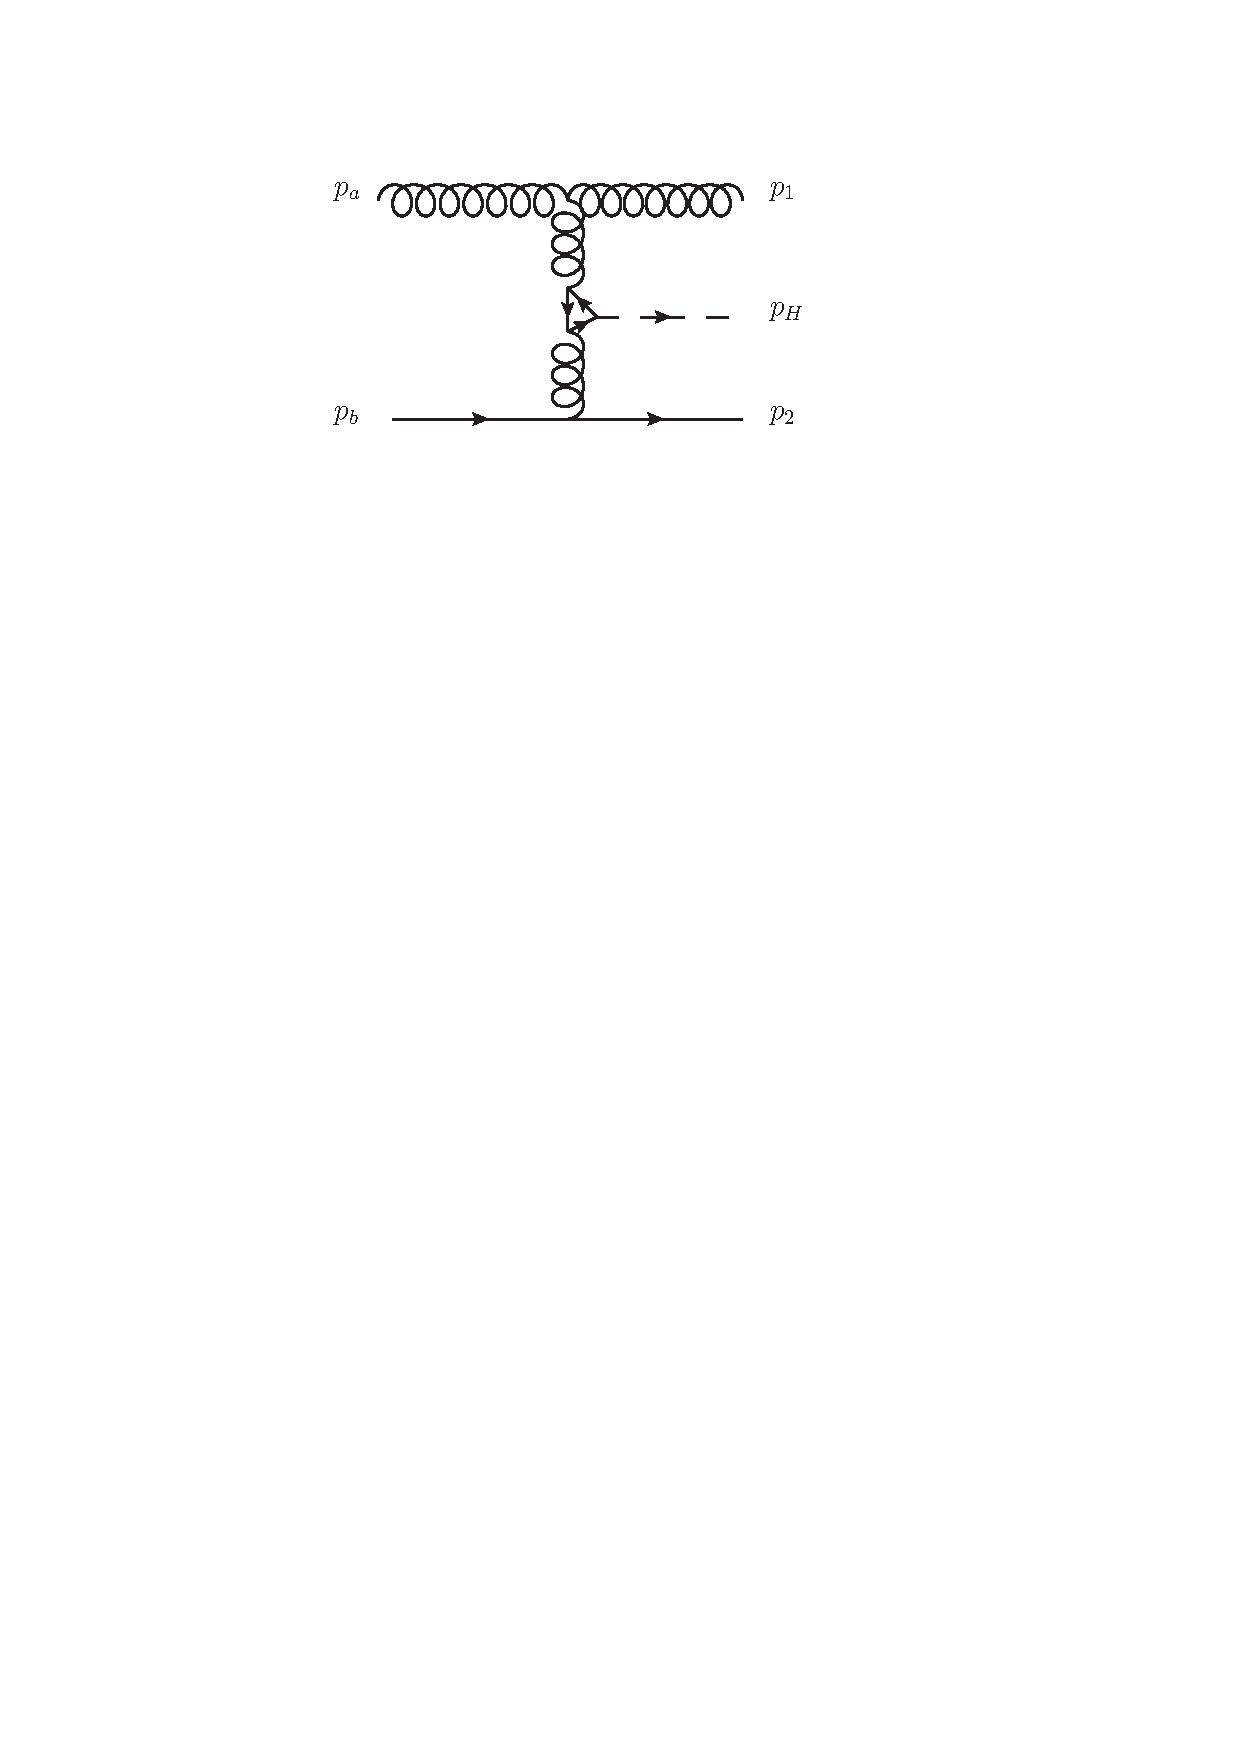
\includegraphics[scale=0.75]{Images/qgh_middle.pdf}} \\
\subfloat{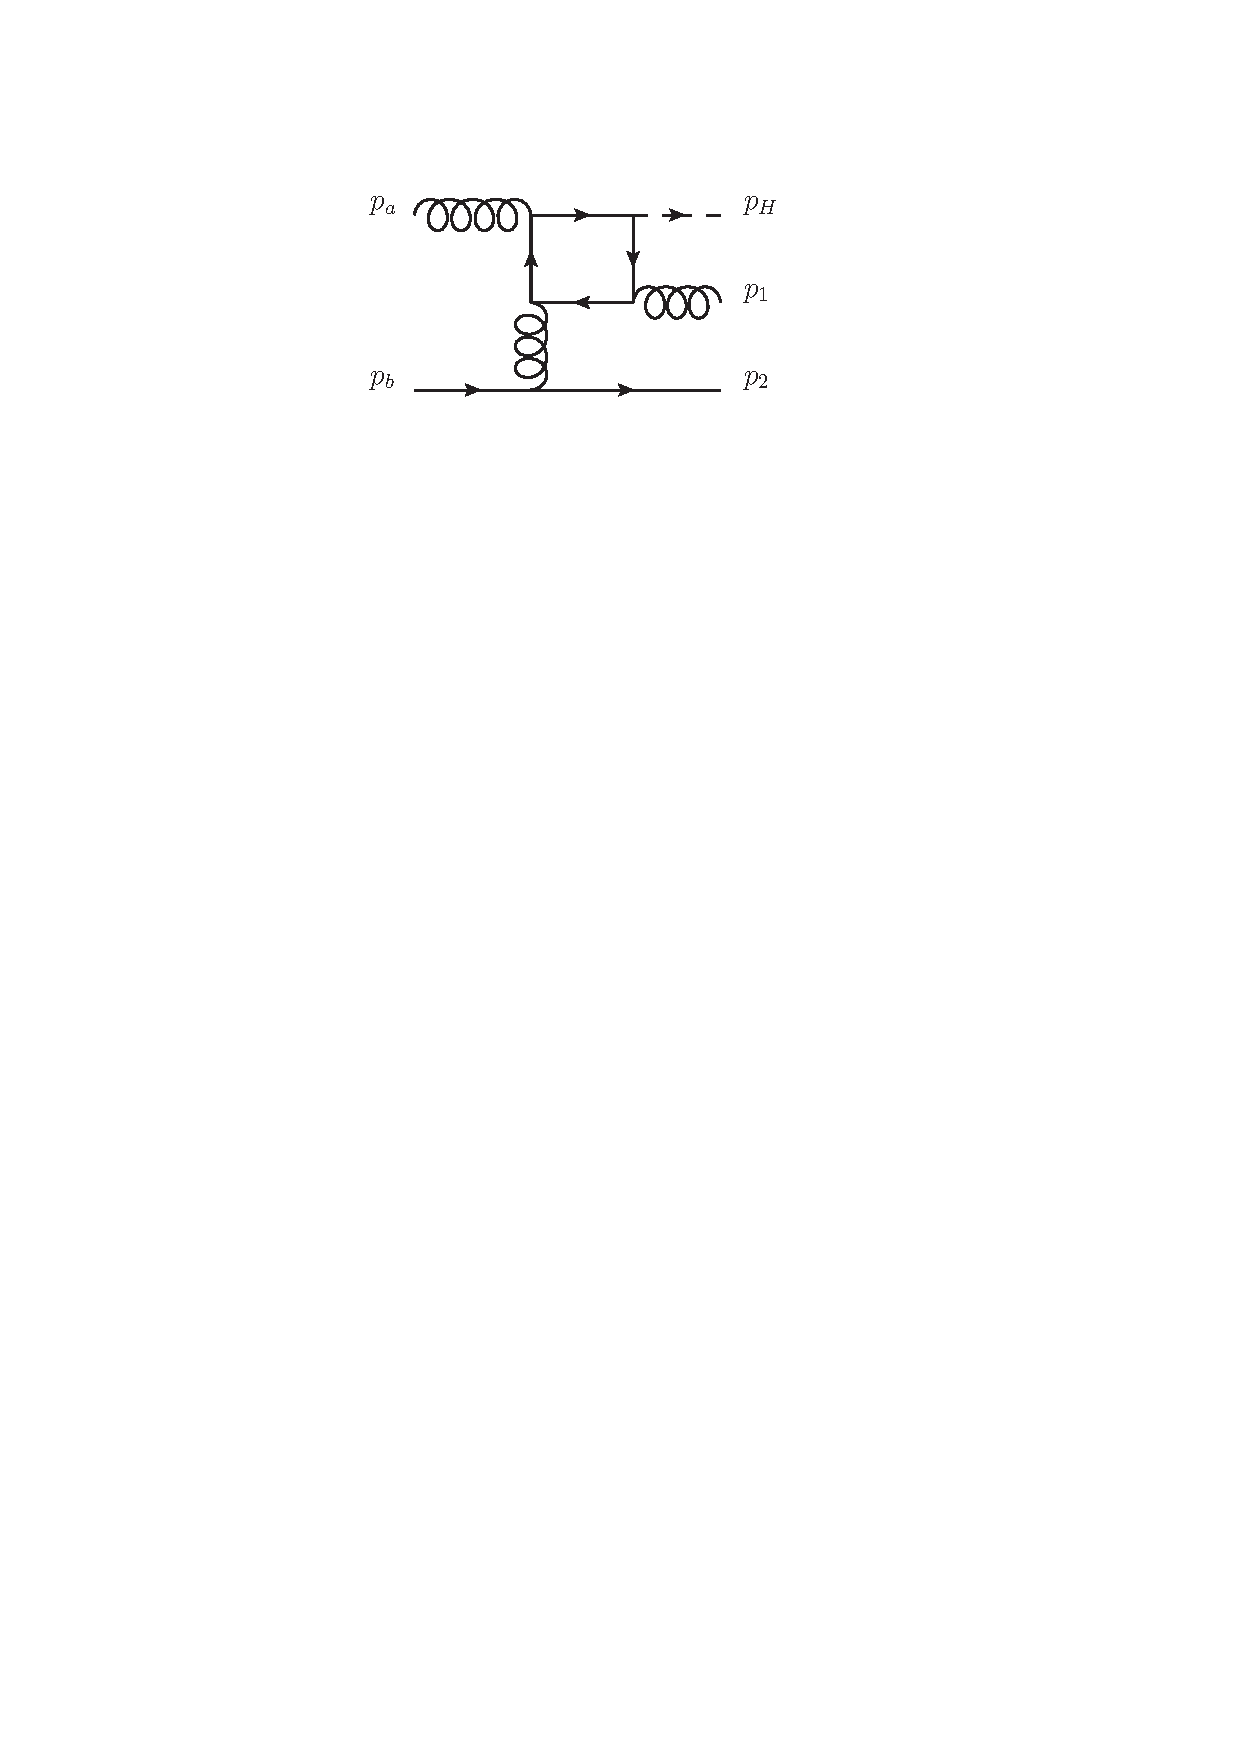
\includegraphics[scale=0.75]{Images/box.pdf}} 
\subfloat{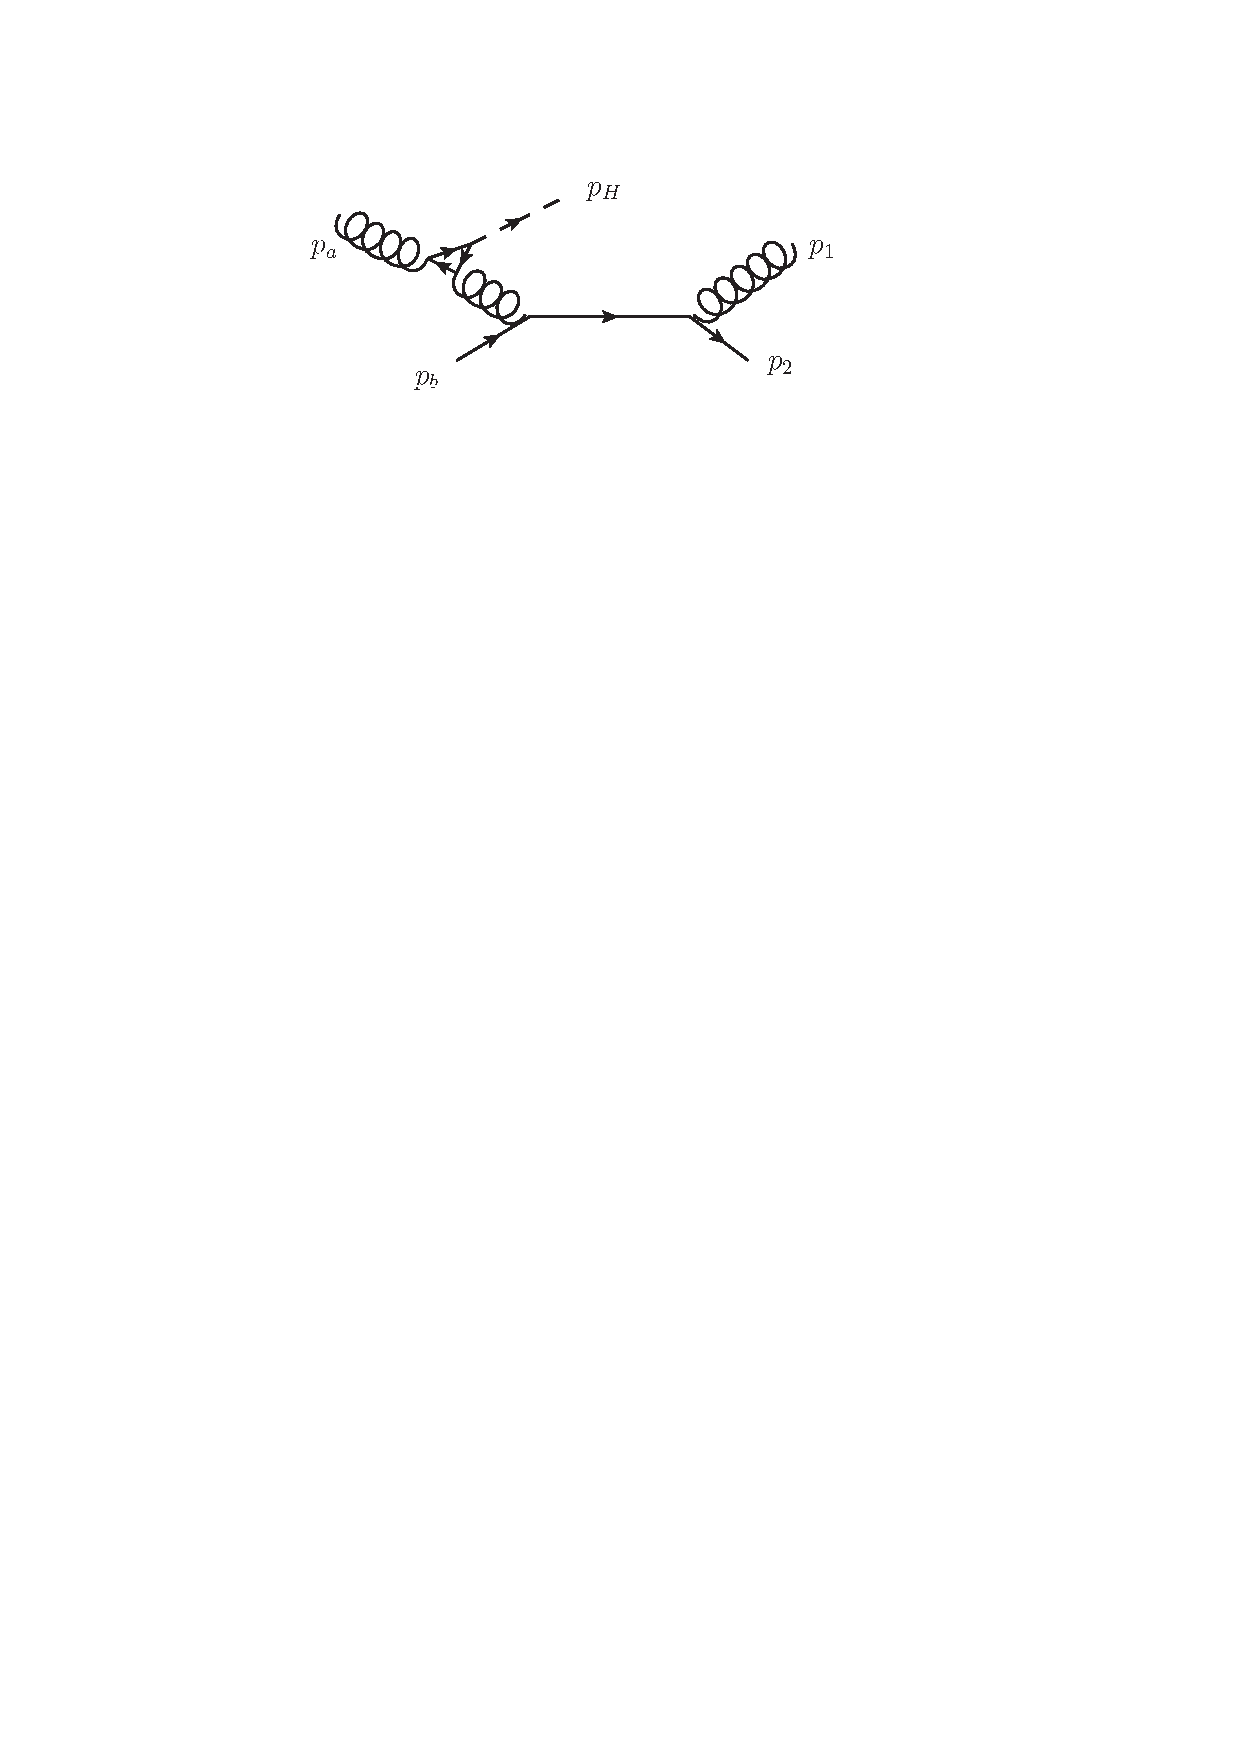
\includegraphics[scale=0.75]{Images/qgh_s.pdf}} \\
\subfloat{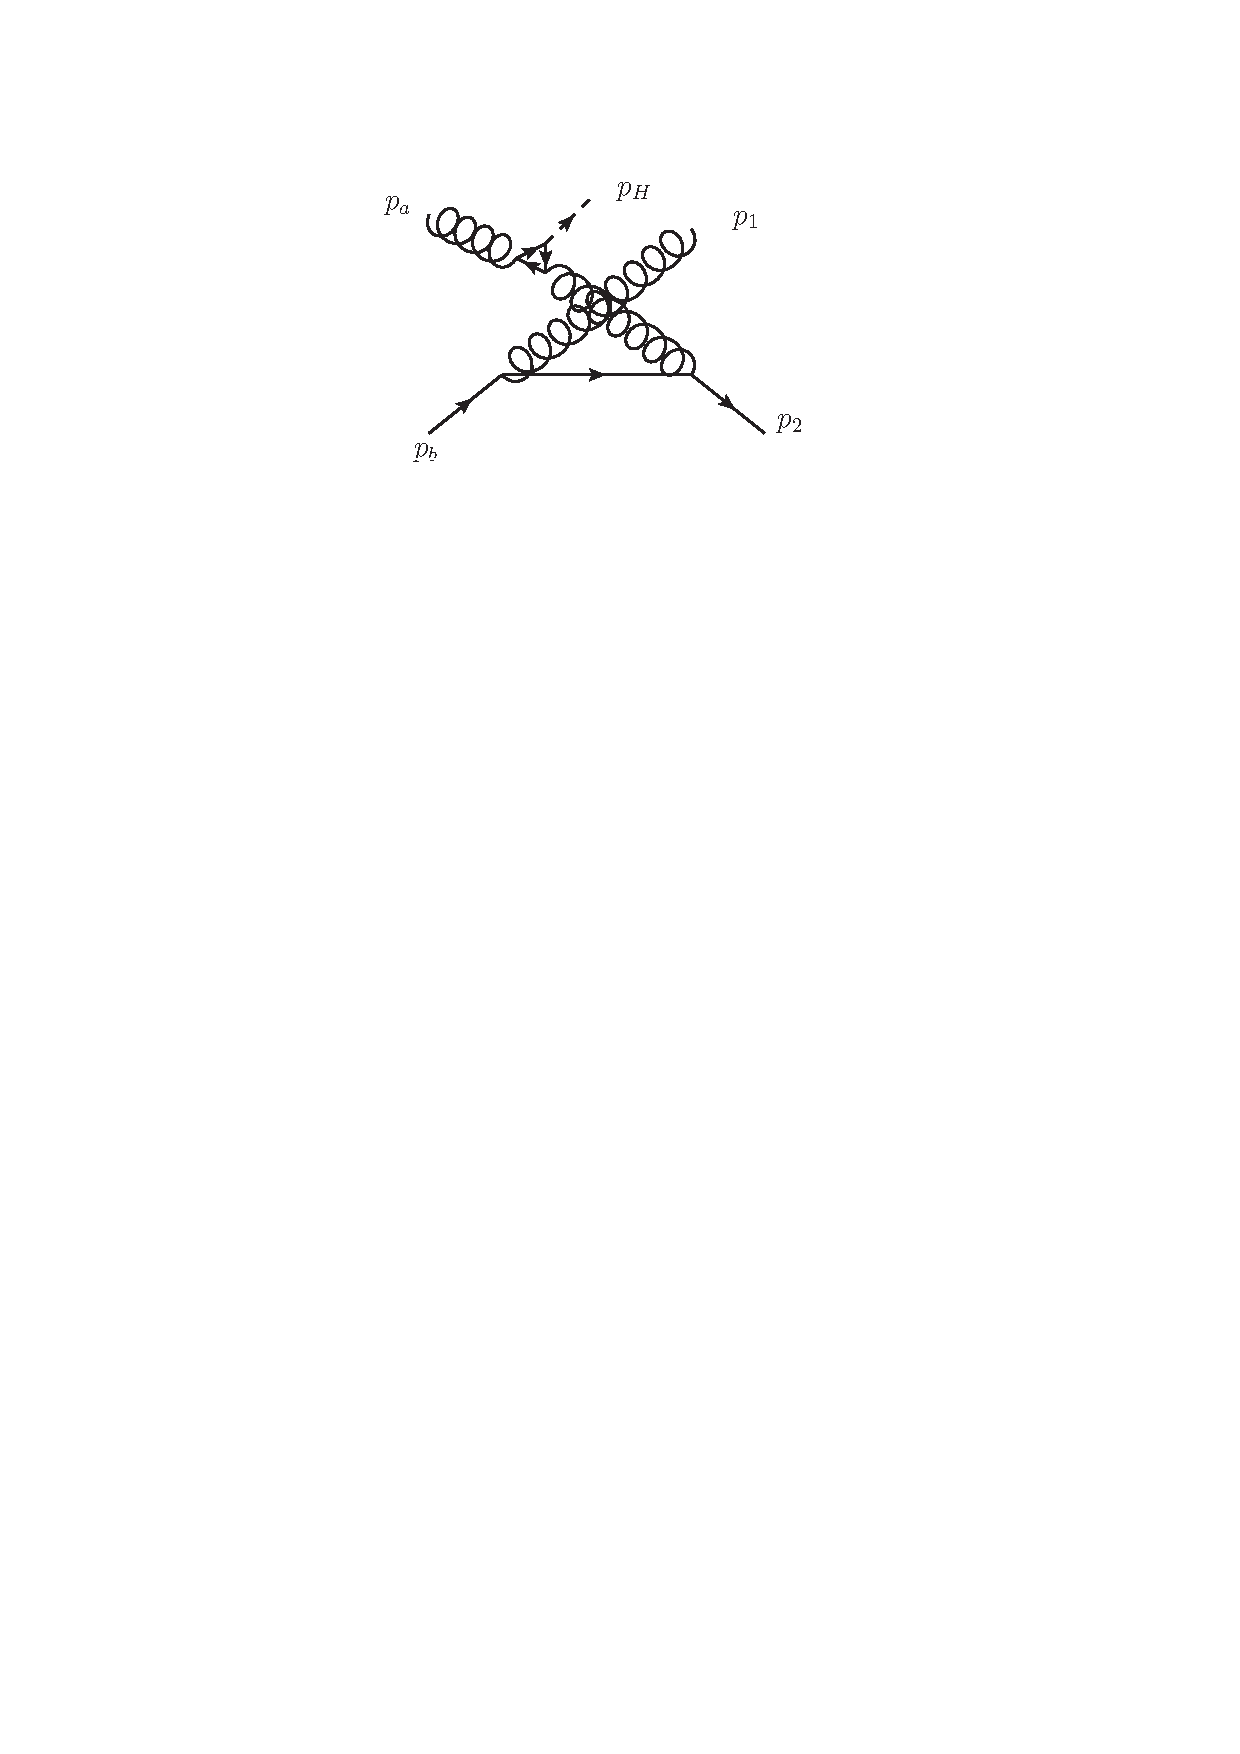
\includegraphics[scale=0.75]{Images/qg_qgh_u.pdf}}
\caption{A selection of LO graphs for $gq \to Hgq$.}
\label{fig:qgh_lo}
\end{figure}
%\todo{Make this nicer, perhaps add a few more. All 10 graphs, maybe? Or 8, if we just have one box.}

where we have $ T_T^{\mu_1 \mu_2} = q_1 \cdot q_2 \eta^{\mu_1 \mu_2} - q_1^{\mu_2} q_2^{\mu_1} $ and $T_L^{\mu_1 \mu_2} = q_1^2 q_2^2 \eta^{\mu_1 \mu_2} - q_1^2 q_2^{\mu_1} q_2^{\mu_2} - q_2^2 q_1^{\mu_1} q_1^{\mu_2} + q_1 \cdot q_2 q_1^{\mu_1} q_2^{\mu_2}$ and both $q_1$ and $q_2$ are going out from the triangle loop. In our calculation, we will thus need to remember to switch the sign of some momenta at points. The full forms for the $F_L$ and $F_T$ functions are;

\begin{equation}
\begin{split}
F_L(q_1^2,q_2^2,Q^2) &= -\frac{1}{2 \text{det} \mathcal{Q}_2} \bigg \{ \left[2-\frac{3 q_1^2 q_2 \cdot Q}{2 \text{det}\mathcal{Q}_2} \right] \left(\tilde{B}_0(q_1)-\tilde{B}_0(Q) \right)\\
&+ \left[2-\frac{3 q_2^2 q_1 \cdot Q}{2 \text{det}\mathcal{Q}_2} \right] \left(\tilde{B}_0(q_2)-\tilde{B}_0(Q) \right) \\
&- \left[4m_t^2 + q_1^2 + q_2^2 + Q^2 - \frac{3 q_1^2 q_2^2 Q^2}{\text{det}\mathcal{Q}_2} \right] \tilde{C}_0(q_1,q_2) \bigg \},
\end{split}
\end{equation}

where $\text{det} \mathcal{Q}_2 =q_1^2q_2^2 - (q_1 \cdot q_2)^2$. The scalar integrals with the tilde notation are related to the scalar integrals shown in equation \ref{eqn:scalars} by multiplying the latter by $-16i\pi^2$ and the $F_L$ and $F_T$ functions are related to the $A_1$ and $A_2$ of equation \ref{eqn:afuncs} by;

\begin{equation}
\begin{split}
A_1(q_1,q_2) &= \frac{i}{(4 \pi)^2}F_T(q_1,q_2), \\
A_2(q_1,q_2) &= \frac{i}{(4 \pi)^2}\left(F_T(q_1,q_2) q_1 \cdot q_2 + F_L(q_1,q_2)q_1^2q_2^2 \right).
\end{split}
\end{equation}

An interesting point to notice is that, if one of the momenta $q_1$ or $q_2$ is on-shell, we only get a contribution from the $F_T$ term in $T^{\mu \nu}$. This comes about because the presence of an on-shell momenta must mean that the vertex is going to be contracted with the relevant polarisation vector, setting the term proportional to $F_L$ to zero. When this happens, we will write $T_R$ in place of $T$ to remind ourselves of this. Finally, since we know that every graph is contributing at the same order in $\alpha_s$, has a Yukawa coupling from the top loop and has factors from loop integrals, we conveniently define;

\begin{equation}
 F = \frac{4 m_t^2}{v} \alpha_s^2, 
\end{equation}

and multiply $F$ into every graph as in \cite{DelDuca2001}. This slightly changes the Feynman rules for QCD that we should use in that all coupling information is now removed.\\
\\
We now begin the process of finding the full LO expression. We start with the graph shown in the top left of figure \ref{fig:qgh_lo}, where the Higgs is emitted off of the gluon leg with momentum $p_1$. The Feynman rules yield;

\begin{equation}
\begin{split}
A_1 = -F \varepsilon_{\mu_1}(p_a)f^{a1t}V_{3g}^{\mu_1 \mu_2 \mu_3}(p_a, -p_1-p_H,-p_a+p_1+p_H)\left(\frac{-i \eta_{\mu_2 \mu_4}}{(p_1+p_H)^2}\right) \\
T_R^{\mu_4 \mu_5}(-p_1-p_H, p_1) \varepsilon^*_{\mu_5}(p_1)\left(\frac{-i \eta_{\mu_3 \mu_6}}{\hat{t}_2}\right)(-i)T^t_{2b}\matel{2}{\mu_6}{b},
\end{split}
\end{equation}

which can be cleaned up to give;

\begin{equation}
\begin{split}
A_1 &= \frac{-i Ff^{a1t}T^t_{2b}}{(p_1+p_H)^2 \hat{t}_2} \varepsilon_{\mu_1}(p_a)V_{3g}^{\mu_1 \mu_2 \mu_3}(p_a, -p_1-p_H,-p_a+p_1+p_H) \\
&\cdot T_{R, \mu_2}^{\hspace{15pt} \mu_5}(-p_1-p_H, p_1) \varepsilon^*_{\mu_5}(p_1)\matel{2}{\mu_3}{b}.
\end{split}
\end{equation}

The diagram where the Higgs is emitted off of the gluon with momentum $p_a$ instead follows in essentially the same fashion and we just quote the final result of the calculation here, which is;

\begin{equation}
\begin{split}
A_2 &=  \frac{-iFf^{a1t}T^t_{2b}}{(p_a-p_H)^2 \hat{t}_2} \varepsilon_{\mu_1}(p_a)T_{R, \hspace{3pt} \mu_3}^{\mu_1}(-p_a,p_a-p_H)V_{3g}^{\mu_3 \mu_4 \mu_5}(p_a-p_H,-p_1,-p_a+p_H+p_1) \\
& \cdot \varepsilon^*_{\mu_4}(p_1)\matel{2}{\mu_5}{b}.
\end{split}
\end{equation}

We now look at the case where the Higgs is emitted from a t-channel gluon, as shown in the top right of figure \ref{fig:qgh_lo}. The Feynman rules give us;

\begin{equation}
\begin{split}
A_3 &= -F \varepsilon_{\mu_1}(p_a)f^{a1t}V_{3g}^{\mu_1 \mu_2 \mu_3}(p_a, -p_1, p_1 - p_a) \left(\frac{-i \eta_{\mu_3 \mu_4}}{(p_a-p_1)^2}\right) \varepsilon_{\mu_2}^*(p_1)\\
&\cdot T^{\mu_4 \mu_5}(p_1-p_a,p_a-p_1-p_H)\left(\frac{-i \eta_{\mu_5 \mu_6}}{\hat{t}_2} \right) (-i)T^t_{2b}\matel{2}{\mu_6}{b},
\end{split}
\end{equation}

which tidies up to;

\begin{equation}
\begin{split}
A_3 &= \frac{-iF f^{a1t}T^t_{2b}}{(p_a-p_1)^2 t_2} \varepsilon_{\mu_1}(p_a)V_{3g}^{\mu_1 \mu_2 \mu_3}(p_a, -p_1, p_1 - p_a)  \varepsilon_{\mu_2}^*(p_1)\\
& \cdot T_{\mu_3}^{\hspace{5pt}\mu_5}(p_1-p_a,p_a-p_1-p_H) \matel{2}{\mu_5}{b}.
\end{split}
\end{equation}

All of these three diagrams have had fairly complicated forms but are automatically factorised in the form we are searching for and so require no further work. The graph involving a box integral will also be like this, but we skip over that calculation for now due to the more complicated nature of it. We will instead discuss the other four diagrams which involve an $s$ or $u$ channel quark propagator. One such diagram is shown in the middle-right of figure \ref{fig:qgh_lo}. The Feynman rules for this diagram give;

\begin{equation}
\begin{split}
A_4 &= -i FT^{1}_{2q} \varepsilon_{\mu_1}^*(p_1) \bar{u}_2 \gamma^{\mu_1}  \left(\frac{i(\slashed{p}_1+\slashed{p}_2)}{s_{12}}\right) \gamma^{\mu_2}u_b (-i)T^{a}_{qb} \left(\frac{-i \eta_{\mu_2 \mu_3}}{(p_a-p_H)^2} \right)\\
&\cdot T_R^{\mu_4 \mu_3}(-p_a,p_a+p_H)\varepsilon_{\mu_4}(p_a),
\end{split}
\end{equation}

which one can tidy up to yield;

\begin{equation}
A_4 = \frac{- F T^1_{2q}T^a_{qb}}{s_{12}(p_a-p_H)^2} \varepsilon^*_{\mu_1}(p_1) \bar{u}_2 \gamma^{\mu_1}(\slashed{p}_1+\slashed{p}_2)\gamma^{\mu_2}u_b T_{R \hspace{2pt} \mu_2}^{\mu_4}(-p_a,p_a-p_H)\varepsilon_{\mu_4}(p_a).
\end{equation}


We have a similar diagram to this where there is still an $s$-channel quark but now the Higgs is emitted off of the $p_1$ leg. The calculation is almost identical so we just quote the result which is;

\begin{equation}
A_5 = \frac{- F T^1_{2q}T^a_{qb}}{s_{ab}(p_1+p_H)^2} \varepsilon_{\mu_2}(p_a) \bar{u}_2 \gamma^{\mu_1}(\slashed{p}_a+\slashed{p}_b)\gamma^{\mu_2}u_b T_{R \hspace{2pt}  \mu_1}^{\hspace{10pt} \mu_4}(-p1-p_H,p_1)\varepsilon_{\mu_4}^*(p_1).
\end{equation}

Finally, we have the u-type diagrams. One such is shown at the bottom of figure \ref{fig:qgh_lo}. The Feynman rules yield;

\begin{equation}
\begin{split}
A_6 &=-FT^a_{2q}T^1_{qb} \bar{u}_2 \gamma^{\mu_1}\left(\frac{i(\slashed{p}_b - \slashed{p_1})}{-s_{b1}} \right)\gamma^{\mu_2}u_b \varepsilon_{\mu_1}^*(p_1)\left(\frac{-i \eta_{\mu_2 \mu_3}}{(p_a-p_H)^2}\right)\\
& \cdot T_R^{\mu_4 \mu_3}(-p_a,p_a+p_H)\varepsilon_{\mu_4}(p_a).
\end{split}
\end{equation}

This can be simplified to;

\begin{equation}
A_6 = \frac{F T^a_{2q}T^1_{qb}}{s_{1b}(p_a-p_H)^2} \bar{u}_2 \gamma^{\mu_1} (\slashed{p}_b - \slashed{p}_1)u_b \varepsilon_{\mu_1}^*(p_1)T_{R \hspace{2pt} \mu_2}^{\mu_4}(-p_a,p_a+p_H)\varepsilon_{\mu_4}(p_a).
\end{equation}

The last diagram is the same as this one except with the Higgs emitted off of the gluon with momentum $p_1$ and the result is;

\begin{equation}
A_7 = \frac{F T^a_{2q}T^1_{qb}}{s_{2a}(p_1+p_H)^2} \bar{u}_2 \gamma^{\mu_1} (\slashed{p}_2 - \slashed{p}_a)u_b \varepsilon_{\mu_1}(p_a)T_{R \hspace{2pt} \mu_2}^{\hspace{12pt} \mu_4}(-p_1-p_H,p_1)\varepsilon^*_{\mu_4}(p_1)
\end{equation}

We now return to the box integrals. There are three independent contributions, related to the three different ways the two gluons and one Higgs can be attached to the box. For ease, we use the parametrisation as described in \cite{Duca2003} (not as in \cite{DelDuca2001}, though they are of course related), which writes this part of the amplitude as;

\begin{equation}
M^{\mu \nu \rho} = \frac{2 g_s^3 mt^2}{v} i f^{bac}T^c J^{\mu \nu \rho}(q_1,q_2,q),
\end{equation}

in their notation. To get from their paper to this thesis we make the following mapping for momenta;

\begin{subequations}
\begin{align}
q_1 &= p_1, \\
q_2 &= - p_a, \\
q &= p_a-p_1-p_H = p_2-p_b,
\end{align}
\end{subequations}

and for the colour indices we map $a \to 1, b \to a, c\to t$. The last thing to do is to write this factor as also proportional to $F$;

\begin{equation}
M^{\mu \nu \rho} = \left(F \times \frac{-16 \pi^2}{2 g_s} \right) f^{a1t}J^{\mu \nu \rho}.
\end{equation}

A very important thing to notice here is that the paper this result is taken from has loop integrals defined with an overall factor of $\frac{1}{(2 \pi)^4}$, whereas the loops used in LoopTools \cite{Hahn1999} (which is the program we will use in the Monte Carlo integration) and \cite{DelDuca2001} are defined with an overall factor of $\frac{1}{i \pi^2}$. We take care of this by simply reweighing the LoopTools results when called here. For brevity, we will write the expression for J in terms of the $q$s rather than the momenta of the external particles. Lifting the expression from this paper also forces us to use a particular gauge, which is the one where the polarisation vector of the gluon with momenta $p_a$ is perpendicular to $p_1$ and vice versa. Imposing this and the function $J$ is;% \todo{Do I need to care about gauge invariance still?}

\begin{equation}
J^{\mu \nu \rho} = \eta^{\mu \nu}(H_1 q_1^\rho + H_2 q_2^\rho) + \eta^{\mu \rho}H_4 q^\nu + \eta^{\nu \rho}H_5 q^\mu + H_{10} q_2^\rho q^\mu q^\nu + H_{12} q_1^\rho q^\mu q^\nu.
\label{eqn:boxes}
\end{equation}

The full expressions for each of the $H$ functions are very long and so we will leave their forms for Appendix A. A useful study is to investigate the link between the finite and infinite top mass cases for the box diagrams. This will, for example, give us a stringent numerical check on our implementation. In the infinite top mass case, the box diagram goes over to a three gluon vertex diagram multiplied by a factor, since the limit shrinks quark loops. Using this knowledge and applying it to the infinite top mass limit of equation \ref{eqn:boxes} along with the factor $F$, we see that the following must hold; 

\begin{equation}
\begin{split}
\frac{2 \pi F}{\alpha_s} H_1 & \to i A, \\
\frac{2 \pi F}{\alpha_s} H_2  &\to -i A, \\
\frac{2 \pi F}{\alpha_s} H_4  &\to i A, \\
\frac{2 \pi F}{\alpha_s} H_5  &\to -i A, \\
\frac{2 \pi F}{\alpha_s} H_{10} &\to 0, \\
\frac{2 \pi F}{\alpha_s} H_{12} &\to 0,
\end{split}
\end{equation}
%\todo{double check this}
with once more $A = \frac{\alpha_s}{3 \pi v}$. This was tested numerically in a computer program by setting $M_t = 174000$ and seen to hold. %There is a factor of $\frac{1}{2}$ here that is not immediately seen in \cite{DelDuca2001}, but we are confident of it.

We can now combine all graphs together. We have three different colour structures appearing from the individual sub-amplitudes, but we use the fact that $[T^a,T^b] = if^{abc}T^c$ to see that we can reduce this down to two. For the time being, we will keep the amplitudes separated into their `natural' colour factor and then later on use our commutator identities. Before we write the full amplitude, we make use of one more useful piece of notation. Throughout the calculation, we came across many instances where one of the polarisation vectors was contracted with a $T_R$ function from the top loop. It will be useful to define an `effective polarisation vector' which is precisely this contraction along with the propagator invariant. In other words;

\begin{subequations}
\begin{equation}
\begin{split}
\frac{\varepsilon_{\mu_1}(p_a)T_{R \hspace{2pt} \mu_2}^{\mu_1}(-p_a, p_a -p_H)}{(p_a-p_H)^2} &= \frac{F_T(p_a^2, (p_a-p_H)^2,p_H^2)\left(p_a \cdot p_H \varepsilon_{\mu_2}(p_a) - p_{a \hspace{2pt} \mu_2} p_H \cdot \varepsilon(p_a)\right)}{(p_a-p_H)^2} \\
& \equiv \varepsilon_{H, \mu_2}(p_a),
\end{split}
\end{equation}
\begin{equation}
\begin{split}
\frac{\varepsilon_{\mu_1}^*(p_1)T_{R \hspace{1pt} \mu_2}^{ \hspace{10pt} \mu_1}(-p_1 - p_H, p_1)}{(p_1+p_H)^2} &= \frac{F_T((p_1+p_H)^2,p_1^2,p_H^2)\left(p_H \cdot \varepsilon^*(p_1) p_{1 \hspace{2pt} \mu_2} - p_1 \cdot p_H \varepsilon^*_{\mu_2}(p_1))\right)}{(p_1+p_H)^2} \\
& \equiv \varepsilon^*_{H, \mu_2}(p_1).
\end{split}
\end{equation}
\end{subequations}

Note that the idea of the effective polarisation tensor has been taken from \cite{DelDuca2001}, but the forms look quite different due to the differences between incoming/outgoing momenta. The full amplitude is then;

\begin{equation}
\begin{split}
M_{gq \to Hgq}^{m_t} = F &\biggl( T^a_{2q}T^1_{qb} \biggl[ \frac{ \bar{u}_2 \gamma^{\mu_1} (\slashed{p}_2 - \slashed{p}_a ) \gamma^{\mu_2} u_b \varepsilon_{\mu_1} (p_a) \varepsilon_{H,\mu_2}^*(p_1)}{s_{2a}} \\
&+ \frac{\bar{u}_2 \gamma^{\mu_1} (\slashed{p}_b - \slashed{p}_1)\gamma^{\mu_2}u_b \varepsilon_{H,\mu_1}(p_a)\varepsilon^*_{\mu_2}(p_1)}{s_{1b}} \biggr] - \\
&T^1_{2q}T^a_{qb} \biggl[ \frac{\bar{u}_2 \gamma^{\mu_1}(\slashed{p}_a+\slashed{p}_b)\gamma^{\mu_2} u_b \varepsilon_{\mu_2}(p_a)\varepsilon^*_{H,\mu_1}(p_1)}{s_{ab}} \\
& + \frac{\bar{u}_2 \gamma^{\mu_1}(\slashed{p}_1+\slashed{p}_2)\gamma^{\mu_2}u_b \varepsilon_{\mu_1}^*(p_1) \varepsilon_{H,\mu_2}(p_a)}{s_{12}} \biggr]  \\
 &- [T^a, T^1]_{2b} \frac{\matel{2}{\mu_3}{b}}{t_2} \biggl[ 8 i \pi^2 \varepsilon_{\mu_2}(p_a) \varepsilon^*_{\mu_1}(p_1)J^{\mu_1 \mu_2 \mu_3}(p_1,-p_a,p_a-p_1-p_H) \\
&+  \varepsilon_{H,\mu_1}(p_a)V_{3g}^{\mu_1 \mu_2 \mu_3}(p_a-p_H, -p_1, -p_a + p_H + p_1) \varepsilon^*_{\mu_2}(p_1)  \\
&+  \varepsilon_{\mu_1}(p_a)V_{3g}^{\mu_1 \mu_2 \mu_3}(p_a,-p_1-p_H,-p_a+p_1+p_H)\varepsilon_{H,\mu_2}^*(p_1)  \\
&+  \frac{\varepsilon_{\mu_1}(p_a)V_{3g}^{\mu_! \mu_2 \mu_4}(p_a,-p_1,p_1-p_a)\varepsilon^*_{\mu_2}(p_1)T_{\mu_4}^{\hspace{10pt} \mu_3}(p_1-p_a,p_a-p_1-p_H)}{(p_a-p_1)^2} \biggr] \biggr).
\end{split}
\end{equation}

This expression has been checked term-by-term with \cite{DelDuca2001} and \cite{Duca2003} and agreement has been found. With the full amplitude known, we can hope to use limiting arguments to factorise the expression into the form we require. To do this, we need to focus on the first four terms in the amplitude, since the other terms are already in the correct form. These four terms have elements of the desired form within them. To see this, consider the numerator of the first term;

\begin{equation}
A_1^{num} = \bar{u}_2 \gamma^{\mu_1}(\slashed{p}_2-\slashed{p}_a)\gamma^{\mu_2}u_b \varepsilon_{\mu_1}(p_a)\varepsilon^*_{H,\mu_2}(p_1).
\end{equation}

With the completeness relation, we can rewrite the $\slashed{p}$ parts in terms of massless spinors,  $\slashed{p} = \left| p^+ \right> \left<p^+ \right| + \left| p^- \right> \left<p^- \right|$. By considering the action of the projection operator $(1\pm \gamma^5)$ it is simple to see that you only pick out one of these helicity projections, which is the helicity projection corresponding to the helicity of particles $b$ and $2$. Thus we can write the term as;

\begin{equation}
A_1^{num} = \left(\matel{2}{\mu_1}{2}\matel{2}{\mu_2}{b} + \matel{2}{\mu_1}{a}\matel{a}{\mu_2}{b}\right)\varepsilon_{\mu_1}(p_a)\varepsilon^*_{H,\mu_2}(p_1).
\label{eqn:num}
\end{equation}

We recall at this point a useful parametrisation for our gluon polarisation vectors, as detailed in \cite{Dixon1996};

\begin{equation}
\varepsilon_\mu^{\pm}(k,q) = \pm \frac{\matel{q^\mp}{\mu}{k^\mp}}{\sqrt{2} \left<q^\mp | k^\pm \right>},
\end{equation}

where $k$ is the momenta of the gluon and $q$ is an arbitrary, massless, reference momenta which reflects our gauge freedom. This notation is useful because it allows us to apply some of the identities we established in section 1.6 to perform dot products. As previously discussed, the parametrisation of the box function requires that we pick the following gauge for the gluon polarisation vectors;

\begin{equation}
\begin{split}
\varepsilon_\mu^{\pm}(p_a) &= \pm \frac{\matel{1^\mp}{\mu}{a^\mp}}{\sqrt{2} \left<1^\mp | a^\pm \right>}, \\
\varepsilon_\mu^{\pm}(p_1) &= \pm \frac{\matel{a^\mp}{\mu}{1^\mp}}{\sqrt{2} \left<1^\mp | a^\pm \right>}.
\end{split}
\end{equation}

Using this, we can perform the $\mu_1$ contraction in \ref{eqn:num} and see that if the spinor chain and the polarisation vector $\varepsilon(p_a)$ have the same helicity, the second term is identically zero. However, if they have opposite helicity, then the dot product goes like $\left<a 1 \right> [ a 2]$. The first term will instead go like $\left<2 1 \right>[a 2]$. We can think of the square and angled brackets as square roots of invariants, so the ratio of these terms is like $\sqrt{s_{a1}/s_{12}}$. 
Since we are considering the limit where $s_{12}$ is large and $s_{a1}$ not necessarily so, we can then neglect the second term. This will apply also to the $\slashed{p}_a$ part of the third term of the full ampitude and a similar argument can be made for the $\slashed{p}_1$ part of the second term and the $\slashed{p}_1$ part of the fourth. Thus we have now approximated the first four terms as;

\begin{equation}
\begin{split}
\tilde{A} \equiv i F \biggl( T^a_{2q}T^1_{qb} \left[ \frac{ \bar{u}_2 \gamma^{\mu_1} \slashed{p}_2 \gamma^{\mu_2} u_b \varepsilon_{\mu_1} (p_a) \varepsilon_{H,\mu_2}^*(p_1)}{s_{2a}} + \frac{\bar{u}_2 \gamma^{\mu_1} \slashed{p}_b\gamma^{\mu_2}u_b \varepsilon_{H,\mu_1}(p_a)\varepsilon^*_{\mu_2}(p_1)}{s_{1b}} \right]
 - \\
T^1_{2q}T^a_{qb} \left[ \frac{\bar{u}_2 \gamma^{\mu_1}\slashed{p}_b \gamma^{\mu_2} u_b \varepsilon_{\mu_2}(p_a)\varepsilon^*_{H,\mu_1}(p_1)}{s_{ab}} + \frac{\bar{u}_2 \gamma^{\mu_1}\slashed{p}_2\gamma^{\mu_2}u_b \varepsilon_{\mu_1}^*(p_1) \varepsilon_{H,\mu_2}(p_a)}{s_{12}} \right] \biggr).
\end{split}
\end{equation}

Because we will be performing contractions and evaluating spinor brackets with the polarisation vectors, we will rewrite them in a different (though of course equivalent) form that we know for sure conforms with our spinor definitions. The formula we quoted from \cite{Dixon1996} is designed for the case where all momenta are taken as outgoing, so when it comes to writing out these contractions explicitly (not just schematically like we did for the scaling argument) we cannot be confident that the convention is the same. Thus, our polarisation vectors for explicit calculations are;  

\begin{subequations}
\begin{equation}
\varepsilon(p_a)^+ = \frac{\matel{a^-}{\mu}{1^-}}{\sqrt{2} [a 1]} = \frac{\matel{1^+}{\mu}{a^+}}{\sqrt{2} [a1]},
\end{equation}
\begin{equation}
(\varepsilon(p_1)^+)^* = -\frac{\matel{a^-}{\mu}{1^-}}{\sqrt{2} \left<1 a \right>]} = -\frac{\matel{1^+}{\mu}{a^+}}{\sqrt{2} \left<1 a \right>},
\end{equation}
\begin{equation}
\varepsilon(p_a)^- = \frac{\matel{1^-}{\mu}{a^-}}{\sqrt{2} \left<1 a \right>]} = \frac{\matel{a^+}{\mu}{1^+}}{\sqrt{2} \left<1 a \right>},
\end{equation}
\begin{equation}
(\varepsilon(p_1)^-)^* = -\frac{\matel{1^-}{\mu}{a^-}}{\sqrt{2} [a 1]} = -\frac{\matel{a^+}{\mu}{1^+}}{\sqrt{2} [a1]}.
\end{equation}
\end{subequations}

We now expand our expression for $\tilde{A}$ using the completeness relation;

\begin{equation}
\begin{split}
\tilde{A} \equiv F \biggl( T^a_{2q}T^1_{qb} \left[ \frac{2 p_2^{\mu_1} \matel{2}{\mu_2}{b} \varepsilon_{\mu_1} (p_a) \varepsilon_{H,\mu_2}^*(p_1)}{s_{2a}} + \frac{\matel{2}{\mu_1}{b} 2 p_b^{\mu_2} \varepsilon_{H,\mu_1}(p_a)\varepsilon^*_{\mu_2}(p_1)}{s_{1b}} \right]
 - \\
T^1_{2q}T^a_{qb} \left[ \frac{\matel{2}{\mu_1}{b}2p_b^{\mu_2}\varepsilon_{\mu_2}(p_a)\varepsilon^*_{H,\mu_1}(p_1)}{s_{ab}} + \frac{2p_2^{\mu_1}\matel{2}{\mu_2}{b} \varepsilon_{\mu_1}^*(p_1) \varepsilon_{H,\mu_2}(p_a)}{s_{12}} \right] \biggr).
\end{split}
\end{equation}

Note that we have not made any choice on the helicity of the quark line $\matel{2}{\mu}{b}$ nor will we need to; we aim to factor out this string from our expression and the terms $2p_b$ and $2p_2$ will appear regardless of the helicity choice. We will now explicitly calculate the contractions with the polarisation vectors using the same spinor convention as outlined in section 1.6. Since our aim is to remove all $p_b$ and $p_2$ dependence from our effective vertex, it will be useful to consider which spinor bracket combinations are independent of these. Two useful results are (we will assume $p_a$ is moving in the + direction for now, but generalise later);

\begin{subequations}
\begin{equation}
\frac{[1b]}{[ba]} = -\sqrt{\frac{p_1^+}{p_a^+}},
\end{equation}
\begin{equation}
\frac{\left<ba\right>}{\left<1b\right>} = -\sqrt{\frac{p_a^+}{p_1^+}}.
\end{equation}
\end{subequations}

These are exact. However, if we consider the limit $p_2^- \sim p_b^-$ that is still valid here, then we have additional, approximate results we can use. For example;

\begin{equation}
\left<1 2 \right> = \sqrt{p_2^+ p_1^-} e^{i \phi_1} - \sqrt{p_2^- p_1^+}e^{i \phi_2} \approx  - \sqrt{p_2^- p_1^+}e^{i \phi_2},
\end{equation}

where we use the fact that both $p_2^+$ and $p_1^-$ are suppressed in comparison to $p_2^-$ and $p_1^+$. Using this, we also use the results (we will use an equality sign, but remember that the equality is only truly realised in the high energy limit);

\begin{subequations}
\begin{equation}
\frac{[12]}{[a2]} = \sqrt{\frac{p_1^+}{p_a^+}},
\end{equation}
\begin{equation}
\frac{\left<a2\right>}{\left<12\right>} = \sqrt{\frac{p_a^+}{p_1^+}}.
\end{equation}
\end{subequations}

Let us now return to our expression for $\tilde{A}$. We calculate the dot product between the pure momentum term (either $p_b$ or $p_2$) and the polarisation vector. There are two cases we need to consider; firstly, when the helicity of the gluons with momentum $p_a$ and $p_1$ are the same (helicity-conserving) and secondly, when they differ (helicity non-conserving). Though there are of course four total choices for the helicities, we need only consider two, being able to get the other two by parity relations. We start with the helicity-conserving case and choose gluons $a,1$ to both have positive helicity. The first term is; 

\begin{equation}
\begin{split}
 \frac{2 p_2^{\mu_1} \matel{2}{\mu_2}{b} \varepsilon_{\mu_1}^+ (p_a) \varepsilon_{H,\mu_2}^{+,*}(p_1)}{s_{2a}} &= \frac{2 \left<2 a \right> [1 2] \matel{2}{\mu_2}{b}\varepsilon_{H,\mu_2}^{+,*}(p_1)}{\sqrt{2}[a 1] \left<2 a \right> [a 2]} \\
 &= \frac{\sqrt{2}\matel{2}{\mu_2}{b}\varepsilon_{H,\mu_2}^{+,*}(p_1)}{[a1]} \sqrt{\frac{p_1^+}{p_a^+}},
 \end{split}
\end{equation}

and therefore (once we factor out the spinor current) is completely independent of both $p_b$ and $p_2$. Similar results occur with the other three terms and, in fact, terms 1 and 3 and 2 and 4 will become equal. At that point, we can rewrite $\tilde{A}$ as proportional to the colour commutator $[T^a,T^1]$. The result is;

\begin{equation}
\tilde{A}_{++} = \sqrt{2} F [T^a,T^1] \matel{2}{\mu}{b} \left(\sqrt{\frac{p_1^+}{p_a^+}}\frac{\varepsilon_{H,\mu}^{+,*}(p_1)}{[a1]} - \sqrt{\frac{p_a^+}{p_1^+}}\frac{\varepsilon_{H,\mu}^{+}(p_a)}{ \left<1 a \right>} \right).
\end{equation}

For the helicity non-conserving case, we choose the helicity of the gluon with momentum $p_a$ to be positive and the other gluon to have negative helicity, yielding similar results:

\begin{equation}
\tilde{A}_{+-} = \sqrt{2} F [T^a,T^1] \frac{\matel{2}{\mu}{b}}{[a1]} \left(\sqrt{\frac{p_1^+}{p_a^+}}\varepsilon_{H,\mu}^{-,*}(p_1) - \sqrt{\frac{p_a^+}{p_1^+}}\varepsilon_{H,\mu}^{+}(p_a) \right).
\end{equation}

If instead we chose $p_a$ to be moving in the - direction, we find by direction calculation that we need to multiply $\tilde{A}_{++}$ and the first term of $\tilde{A}_{+-}$ by $-\frac{p_{1,\perp}^*}{|p_{1,\perp}|^2}$ and the second term of $\tilde{A}_{+-}$ by $-\frac{p_{1,\perp}}{|p_{1,\perp}|^2}$. \\
\\
We have now achieved our goal of creating a factorised matrix element. Before we write down the explicit expressions for that, we consider if the form can be made to look simpler. For example, in the helicity conserving case, our gauge actually sets one diagram identically zero. The graph shown in the top right of figure \ref{fig:qgh_lo} has a part which is a three-gluon vertex contracted with symmetric polarisation vectors that depend only on the momenta along the top line. It is easy to show by direct calculation that this yields a result of zero. Because we are going to implement this in a numerical integration program, it is important to find these contributions where the analytical result is zero because, depending on the accuracy of the calculation, a computer might give you a small (but vitally non-zero) answer that could potentially hurt your integration. \\
\\
We now have everything we need to state the result of $gq \to Hgq$ in the limit where the Higgs is emitted close to the gluon in rapidity space. For our High Energy expressions, we will present a form which will conform with equation \ref{eqn:higgseff} by performing some of the index contractions. After some manipulation, we find for the helicity conserving amplitude (we will take $p_a$ to be moving in the + direction, but recall that we know how to immediately get to the situation where it is going in the - direction);

\begin{equation}
\begin{split}
A_{++} &= F[T^a,T^1]\frac{\matel{2}{\mu}{b}}{\hat{t}_2} \bigg[\sqrt{\frac{2p_1^+}{p_a^+}}\frac{\varepsilon_{H,\mu}^{+,*}(p_1) \hat{t}_2}{[a1]} - \sqrt{\frac{2p_a^+}{p_1^+}}\frac{\varepsilon_{H,\mu}^{+}(p_a)\hat{t}_2}{ \left<1 a \right>} \\
&+ \frac{\matel{1^+}{H}{a^+}}{\sqrt{2}\left<1 a \right>}\varepsilon_{H,\mu}^+(p_a) + \frac{\matel{1^+}{H}{a^+}}{[a 1]}\varepsilon^{+,*}_{H,\mu}(p_1) \\
&- \frac{\sqrt{2} F_{Ta} p_a \cdot p_1 \matel{1^+}{H}{a^+}}{[a1]}\varepsilon^{+,*}_\mu (p_1) - \frac{\sqrt{2} F_{T1} p_a \cdot p_1 \matel{1^+}{H}{a^+}}{\left<1 a \right>}\varepsilon^+_\mu (p_a)  \\ 
& -\frac{\matel{1^+}{H}{a^+}}{\sqrt{2} [a1]} \varepsilon^{+,*}_\mu(p_1) R H_4 + \frac{\matel{1^+}{H}{a^+}}{\sqrt{2} \left <1 a \right>} \varepsilon^{+}_\mu(p_a)R H_5 \\
 & + \frac{\matel{1^+}{H}{a^+}^2}{2 \left<1 a \right> [a 1]}\left \{ p_{a,\mu} R H_{10} - p_{1,\mu}RH_{12}\right \} \bigg]
\end{split}
\end{equation}

where we have introduced the notation $F_{Ta} = \frac{F_T(0,(p_a-p_H)^2,m_H^2)}{(p_a-p_H)^2}$,  $F_{T1} = \frac{F_T((p_1+p_H)^2, 0, m_H^2)}{(p_1+p_H)^2}$ and $R = 8 i \pi^2$. The part in the square brackets can be interpreted directly (or along with some of the overall constants) as the effective vertex we were searching for, in the helicity conserving case. What remains then, is the helicity non-conserving case which is given by;

\begin{equation}
\begin{split}
A_{+-} &=F[T^a,T^1]\frac{\matel{2}{\mu}{b}}{\hat{t}_2} \bigg[\sqrt{\frac{2p_1^+}{p_a^+}}\frac{\varepsilon_{H,\mu}^{+,*}(p_1) \hat{t}_2}{[a1]} - \sqrt{\frac{2p_a^+}{p_1^+}}\frac{\varepsilon_{H,\mu}^{+}(p_a)\hat{t}_2}{[a1} \\
&+ \frac{\matel{1^+}{H}{a^+}}{\sqrt{2}[a1]}\varepsilon_{H,\mu}^+(p_a) + \frac{\matel{1^+}{H}{a^+}}{[a 1]}\varepsilon^{+,*}_{H,\mu}(p_1) \\
&- \frac{\sqrt{2} F_{Ta} p_a \cdot p_1 \matel{1^+}{H}{a^+}}{[a1]}\varepsilon^{+,*}_\mu (p_1) - \frac{\sqrt{2} F_{T1} p_a \cdot p_1 \matel{1^+}{H}{a^+}}{[a1]}\varepsilon^+_\mu (p_a)  \\ 
& -\frac{\matel{1^+}{H}{a^+}}{\sqrt{2} [a1]} \varepsilon^{+,*}_\mu(p_1) R H_4 + \frac{\matel{1^+}{H}{a^+}}{\sqrt{2} [a1]} \varepsilon^{+}_\mu(p_a)R H_5 \\
 &+ \frac{\matel{1^+}{H}{a^+}^2}{2 [a 1]^2}\left \{ p_{a,\mu} R H_{10} - p_{1,\mu}RH_{12}\right \} \\
 &+ e^{i \phi} R H_1 p_1^\mu - e^{i \phi} R H_2 p_a^\mu + 2 e^{i \phi} F_{T1} p_1\cdot p_H p_a^\mu - 2 e^{i \phi}F_{Ta} p_a \cdot p_H p_1^\mu \\
 &- e^{i \phi} (p_a + p_1)^\mu F_{\alpha} \frac{(p_1-pa)\cdot(p_a-p_1-p_H)}{(p_a-p_1)^2} \\
 &+ e^{i \phi} (p_a - p_1 - p_H) \cdot (p_a + p_1) \frac{(p_1-p_a)}{(p_a-p_1)^2} F_\alpha \\
 &- e^{i \phi} F_\beta (p_a-p_1-p_H)^2 (p_a + p_1)^\mu 
  \bigg]
\end{split}
\end{equation}

where we have $F_\alpha = F_T(p_1-p_a,p_a-p_1-p_H,p_H)$, $F_\beta = F_L(p_1-p_a,p_a-p_1-p_H,p_H)$ and $\varepsilon^{-,*}(p_1) \cdot \varepsilon^+(p_a) = e^{i \phi}$ as the phase factor that comes out of dotting the polarisation vectors. \\
\\
With both the helicity conserving and non-conserving vertices found, we are able to provide a high energy approximation to the whole amplitude by manually performing the colour/helicity sum/average. The colour sum is simple, since the approximation is proportional only to $f^{a1t} T^t$ and, using the normalisation $Tr(T^a T^b) = \frac{1}{2}$, we find that the sum yields an answer of 12. Since we have a quark and gluon incoming, the average factor is $\frac{1}{3 \times 8} = \frac{1}{24}$. For the helicities, there are are total of 8 combinations, of which we need only work out 4 because the other 4 are related by parity and we average by a factor of 4.  This gives our full approximation to be (where the subscripts refer to the helicities of particles with momenta $p_a,p_1,p_2 \hspace{1pt} \& \hspace{1pt} p_b$ respectively and $P$ is the parity operation);

\begin{equation}
\begin{split}
|M_{gq \to Hgq}^{m_t, HE}|^2 &= \frac{1}{8} \big( |A_{++,-}|^2 + |A_{++,+}|^2 + |A_{+-,-}|^2 + |A_{+-,+}|^2 + \\
&|P(A_{++,-})|^2 + |P(A_{++,+})|^2 + |P(A_{+-,-})|^2 + |P(A_{+-,+})|^2 \big).
\end{split}
\end{equation}

\subsection{Checks and Verifications of Amplitudes}

Given recent advances in MadGraph, we are able to check our result against a full LO implementation, complete with finite top mass effects. We first decide to check a phase space configuration where the Higgs boson is kept central in rapidity and the two extremal jets are allowed to move further and further apart. The precise momentum configuration used is; 

\begin{subequations}
\begin{align}
p_1 &= (40 \sqrt{2} \cosh(\Delta),-40,40,40 \sqrt{2} \sinh(\Delta)), \\
p_H &= (\sqrt{40^2+m_H^2}, 0,-40,0), \\
p_2 &= (40 \cosh(-\Delta),40,0,40 \sinh(-\Delta)).
\end{align}
\end{subequations}

This configuration is useful to check against for two reasons. Firstly, it is a more restrictive limit than the one we considered to derive our amplitude (here, $s_{1H}$ also must be large) and so our calculation should correctly describe this situation too. Secondly, High Energy theory tells us that this process should behave like the $qQ \to qHQ$ case where the Higgs is produced far from the parton rapidities with a reweighting due to the quark being replaced by a gluon. Figure \ref{fig:gu_ghu_cen} shows both of these points clearly. 

\begin{figure}[t]
\centering
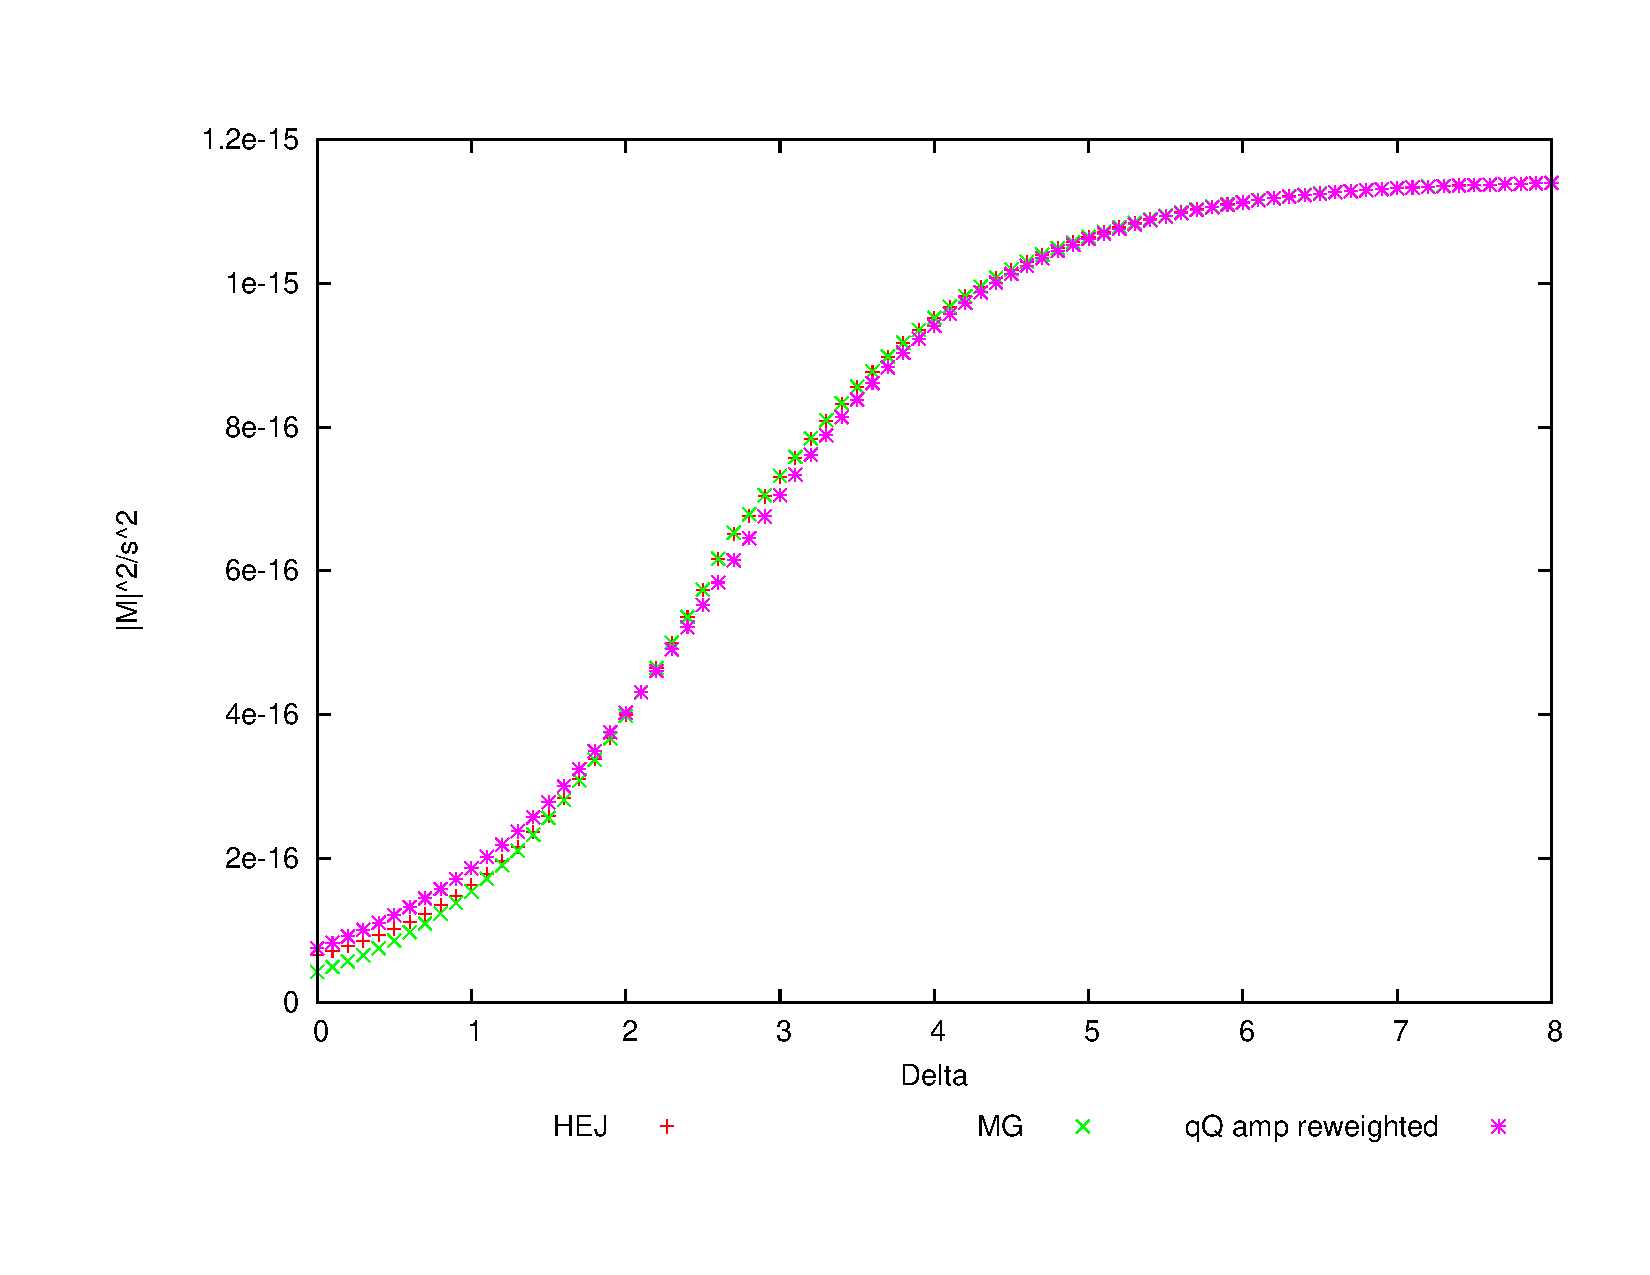
\includegraphics[scale=0.5]{Images/qg_qgH_central.pdf}
\caption{Comparison between the HEJ effective vertex, the full LO result and the result of the $qQ \to qHQ$ LO calculation reweighted by a colour factor for a central H in $gq \to Hgq$ with full top mass dependence.}
\label{fig:gu_ghu_cen}
\end{figure}
%\todo{Make all captions in section nice}
Our second phase space parametrisation fixes the Higgs boson to always be close to the gluon in rapidity whilst the two jets move further apart in rapidity. Explicitly; 

\begin{subequations}
\begin{align}
p_1 &= (40 \sqrt{2} \cosh(\Delta),-40,40,40 \sqrt{2} \sinh(\Delta)), \\
p_H &= (\sqrt{40^2+m_H^2} \cosh(\Delta+0.5), 0,-40,\sqrt{40^2+m_H^2}  \sinh(\Delta + 0.5)), \\
p_2 &= (40 \cosh(-\Delta),40,0,40 \sinh(-\Delta)).
\end{align}
\end{subequations}

In figure \ref{fig:gu_ghu_out}, we plot this new effective vertex approach against the full LO result with this momenta set. We also include the result of the reweighted $qQ \to qHQ$ amplitude to show that this is not an appropriate result in this limit. 

\begin{figure}[t]
\centering
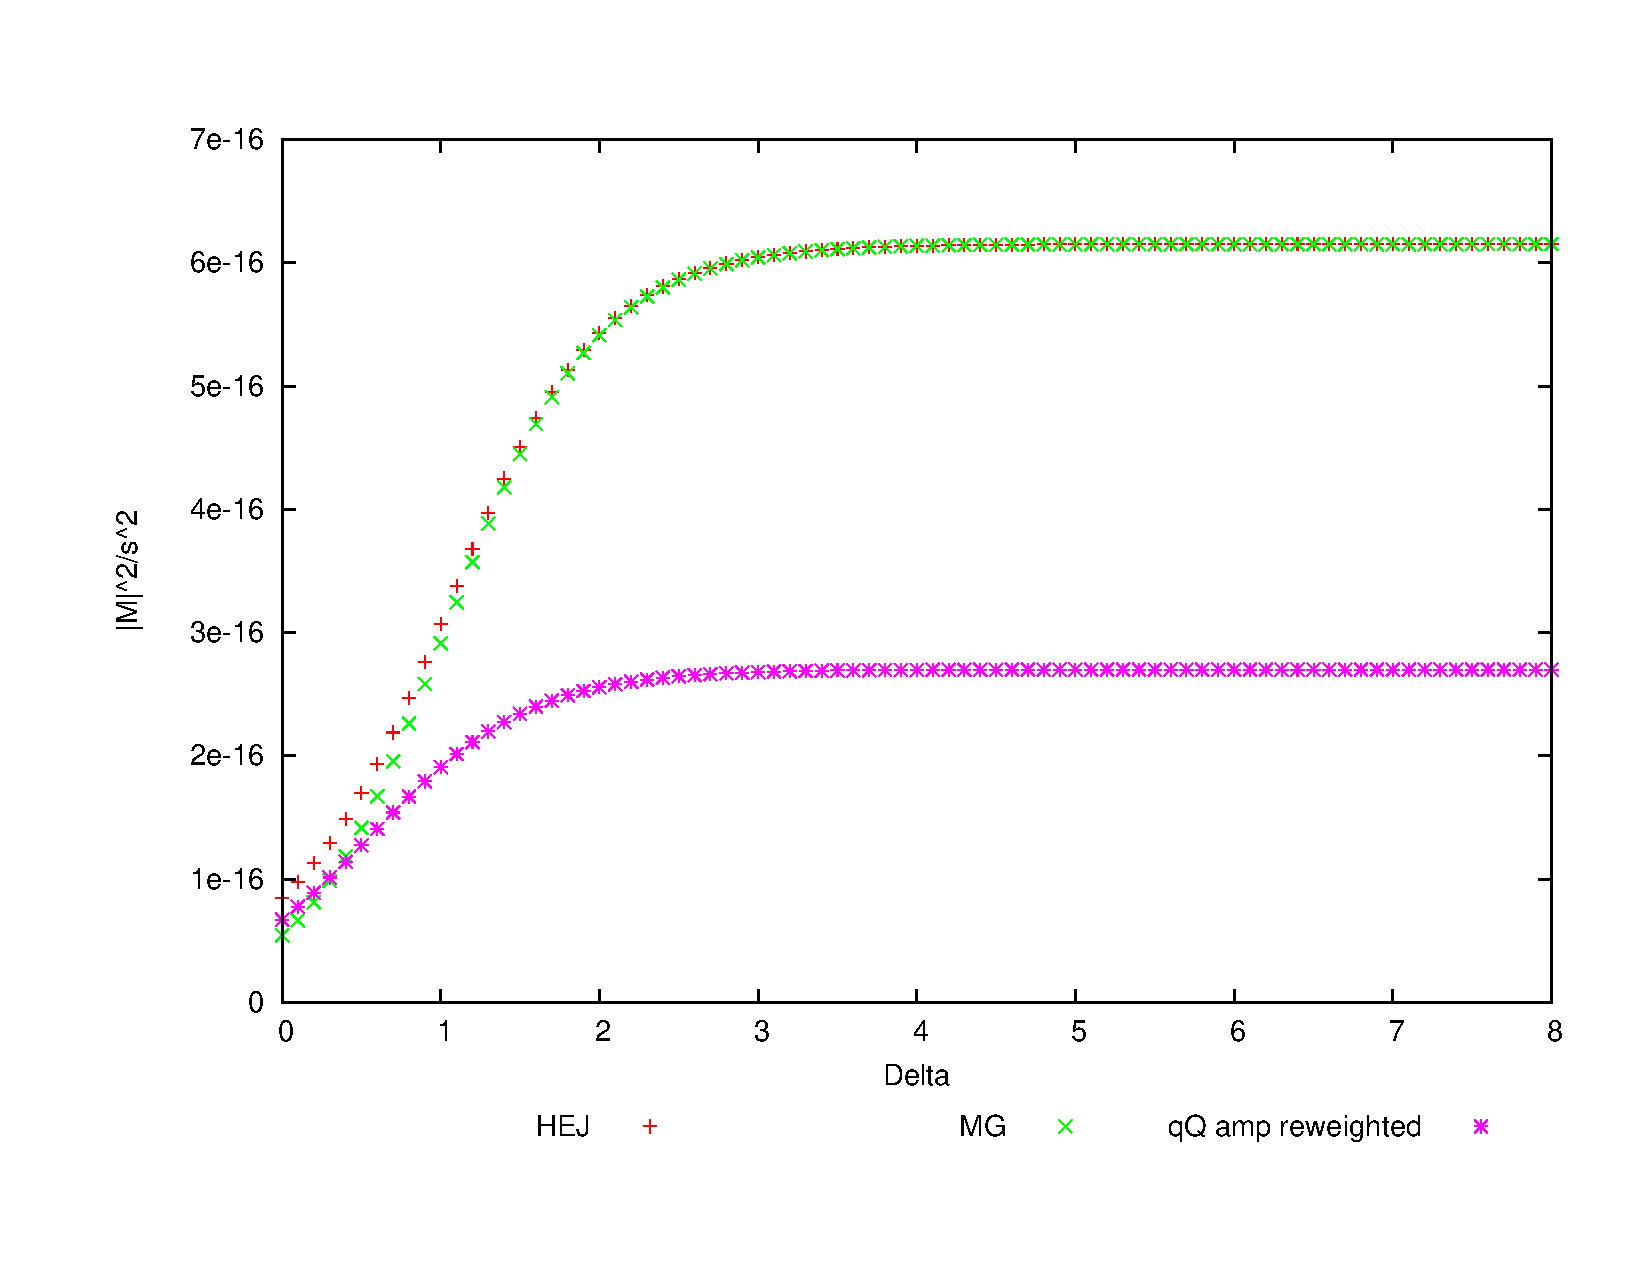
\includegraphics[scale=0.5]{Images/qg_qgH_outside.pdf}
\caption{Comparison between the HEJ effective vertex, the full LO result and the result of the $qQ \to qHQ$ LO calculation reweighted by a colour factor for an outside H in $gq \to Hgq$ with full top mass dependence.}
\label{fig:gu_ghu_out}
\end{figure}

In both cases, we see clear agreement between our result and the full LO result from MadGraph in the high energy limit (high $\Delta$). We now move on to check the effects of having a finite quark mass compared to an infinite one. By simply putting a high value for the top mass in our amplitude (numerically, we see that $m_t = 17400$ is a good choice) we can generate results that correspond to the effective theory where the top mass is treated as an infinite parameter. Additionally, we can very easily add the interference via bottom loops to our result (when working out the amplitudes for helicity configurations, simply add the same amplitude with the bottom mass before squaring it) so we can also see how large an effect this has. We will begin by looking at these three cases with a central Higgs (the first set of momenta), which is plotted in figure \ref{fig:qg_qgh_compare}. We see that there are clear differences between the cases. The finite top mass case is always greater than the infinite top mass case and the addition of the bottom quark makes it larger still. The same comparison for a Higgs close to the gluon (the second set of momenta) is plotted in figure \ref{fig:qg_qgh_compare_out}. In that case, we have slightly different behaviour - the infinite top mass case is still lower, but now the addition of the bottom loop (slightly) decreases the ME from the case where only the top quark is considered. 
%\todo{Fix diagrams to make them sit nicer}
\begin{figure}[t]
\centering
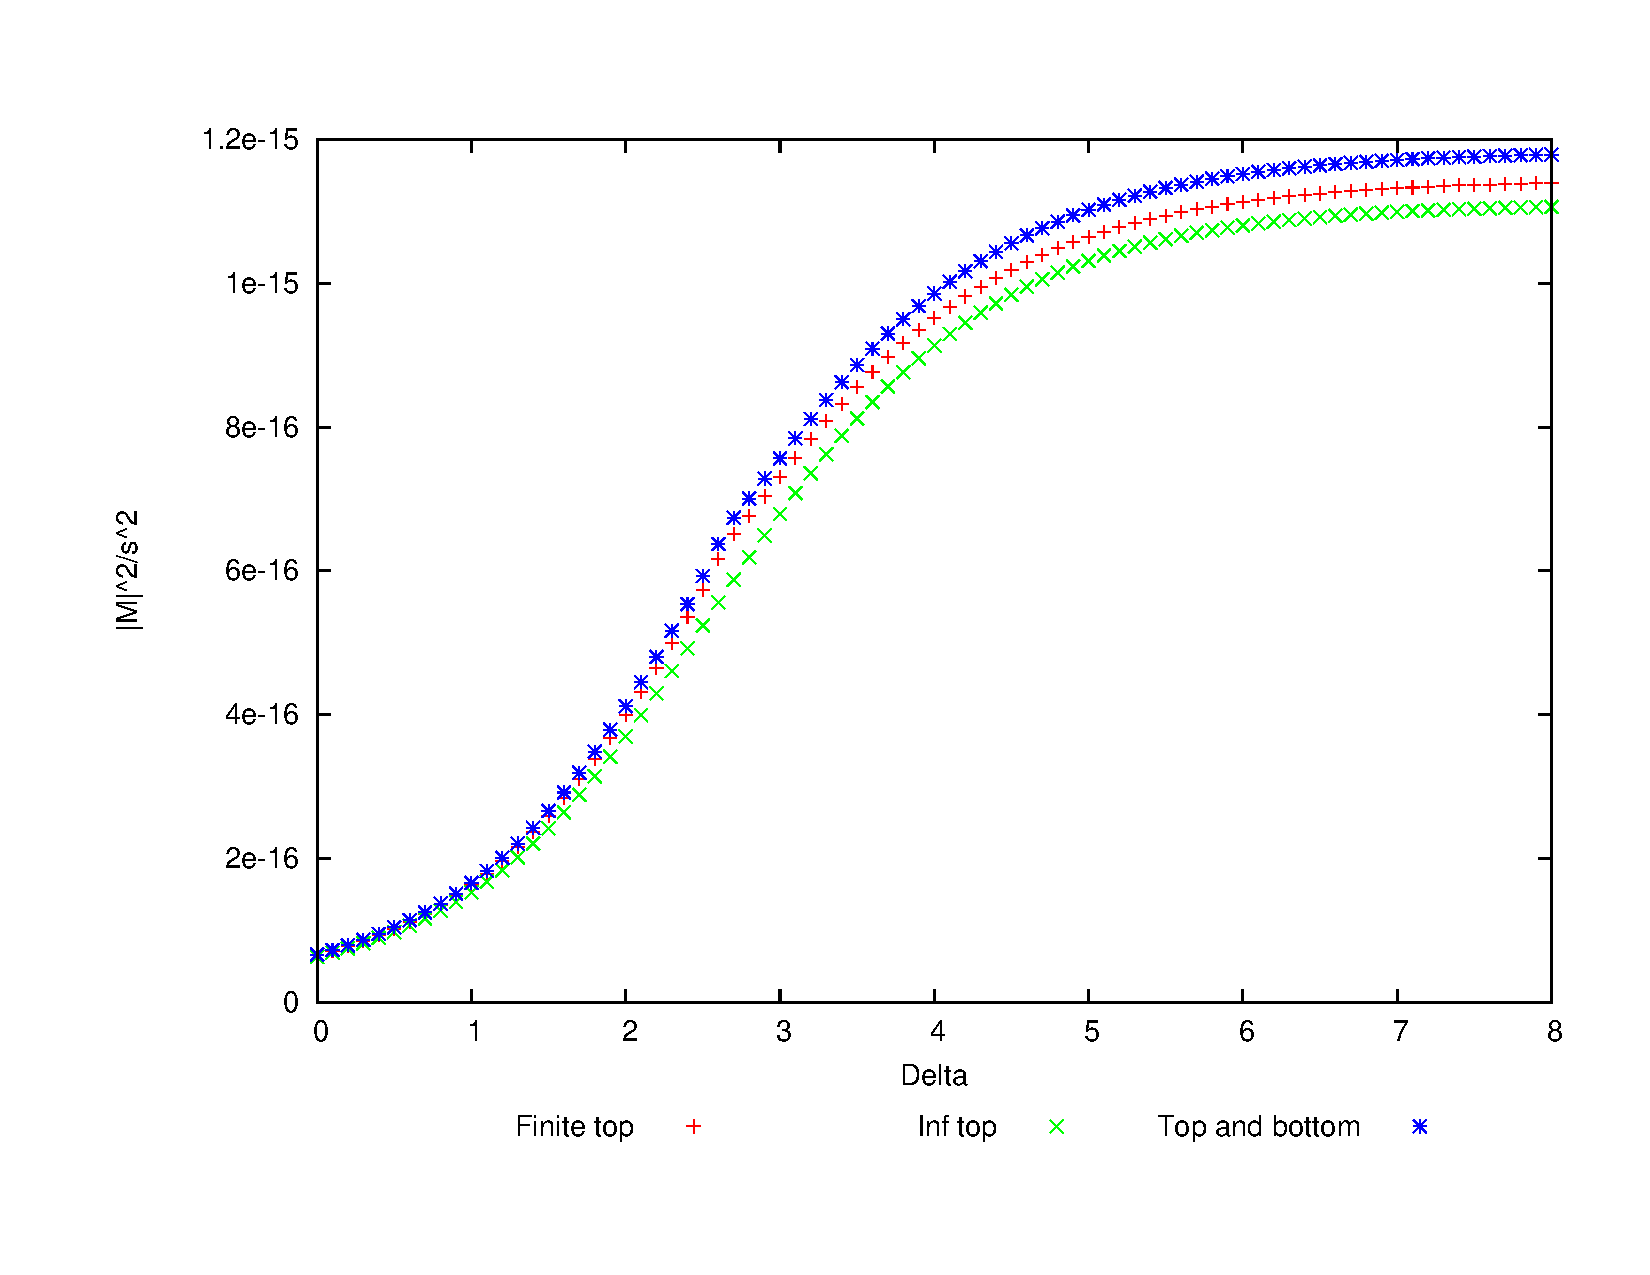
\includegraphics[scale=0.5]{Images/qg_qgH_compare_central.pdf}
\caption{Comparison of infinite top, finite top and finite top plus finite bottom HEJ matrix elements with a central Higgs.}
\label{fig:qg_qgh_compare}
\end{figure}

\begin{figure}[H]
\centering
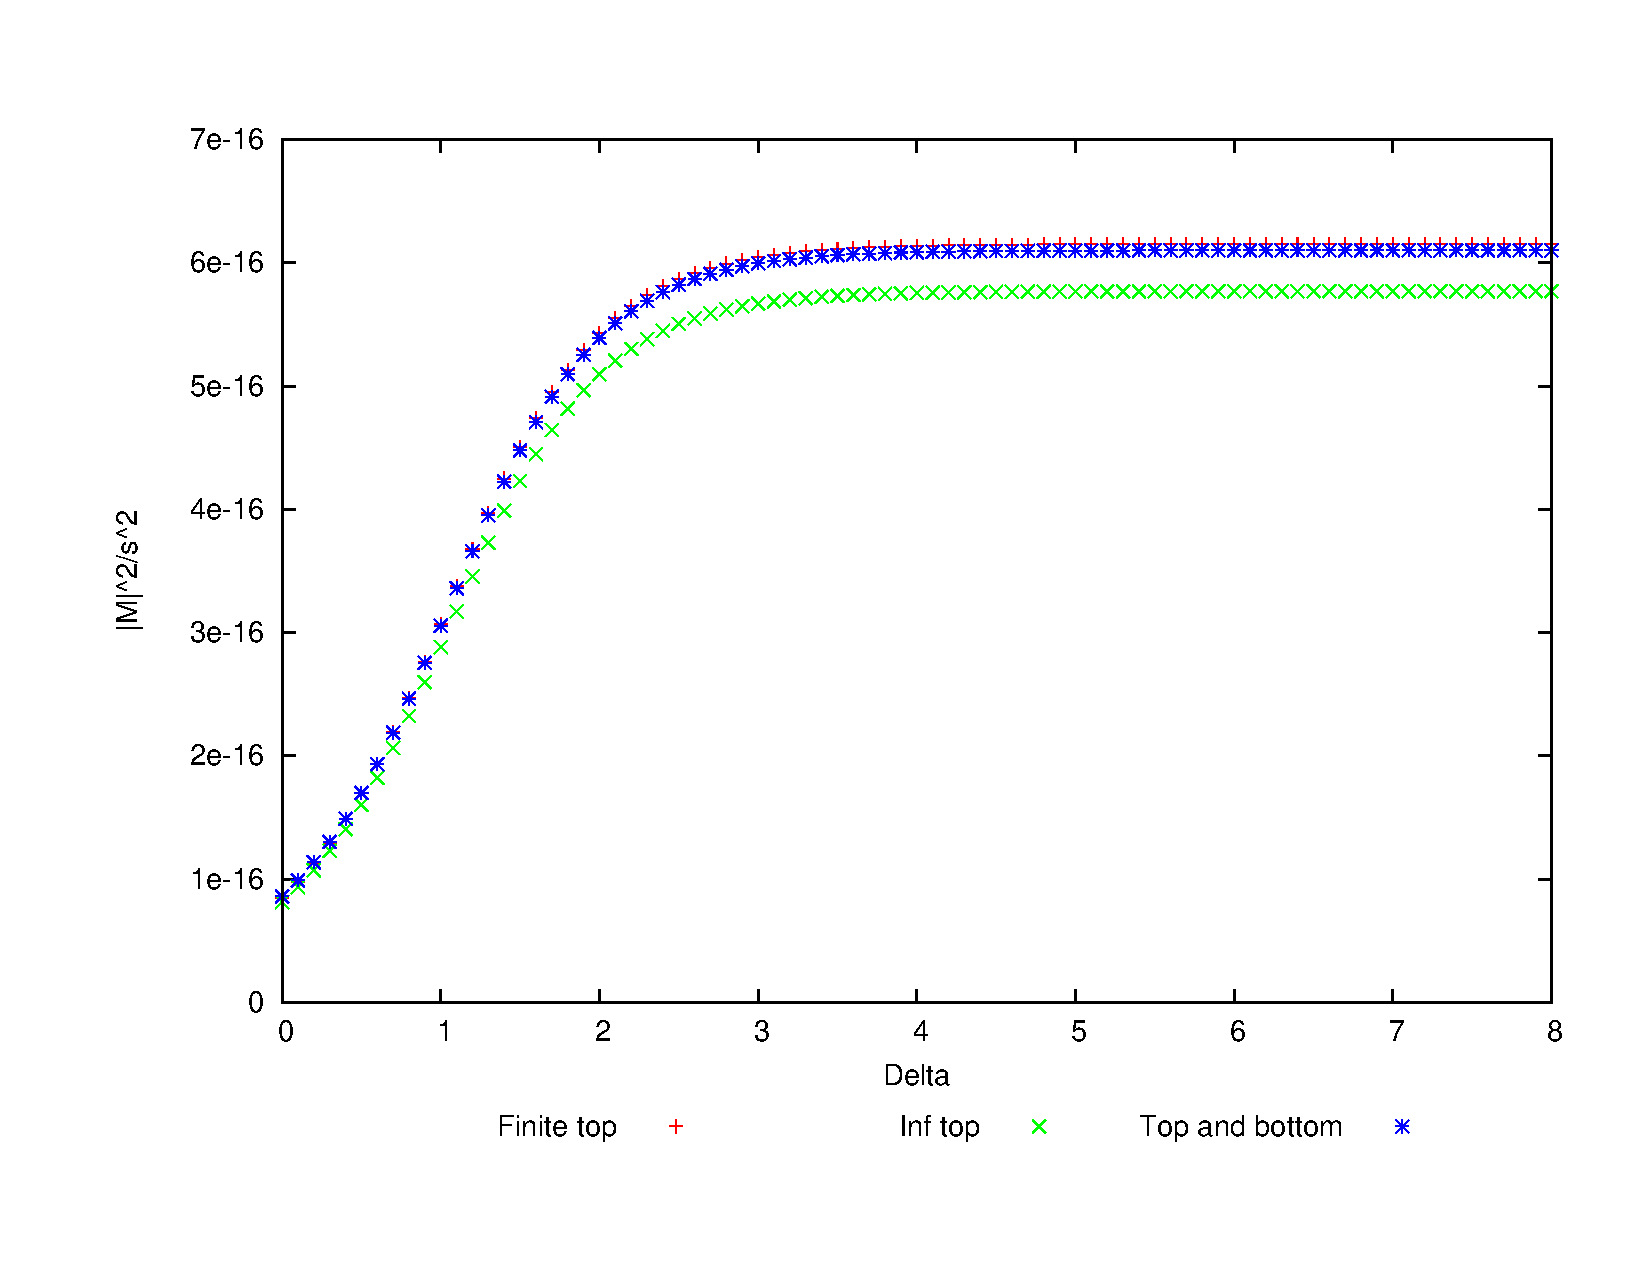
\includegraphics[scale=0.5]{Images/qg_qgH_compare_outside.pdf}
\caption{Comparison of infinite top, finite top and finite top plus finite bottom HEJ matrix elements with an outside Higgs.}
\label{fig:qg_qgh_compare_out}
\end{figure}

The addition of extra emissions is once more done by multiplying Lipatov vertices into the amplitude we have derived. Although some care has to be taken to ensure the correct t-channel momenta are taken, it is relatively straightforward to do this, resulting in a general $gq\to Hg...q$ amplitude (where the ... represent an arbitrary number of gluons) which is simply;

\begin{equation}
|M_{gq \to Hg...q}^{HE,m_t}|^2 = |M_{gq \to Hgq}^{HE,m_t}|^2 \times \prod_{i=1}^{n-2} \frac{-g_s^2C_A V^\mu V_\mu}{\hat{t}_i^2},
\end{equation}

where $n$ is the number of final state jets. As a check, we will generate more explorer plots for the case of one extra emission. We will choose the process $gu \to Hggu$ with a few different choices for the rapidity of the extra gluon and the Higgs to ensure we are calculating correctly. Our first configuration is used for when the Higgs is being emitted close to the extremal gluon;

\begin{subequations}
\begin{align}
p_1 &= (40 \cosh(\Delta),-40,0,40 \sinh(\Delta)), \\
p_H &= (\sqrt{40^2+m_H^2} \cosh(\Delta+0.5), 0,-40,\sqrt{40^2+m_H^2}  \sinh(\Delta+0.5)), \\
p_2 &= (40 \cosh(-\Delta/3),0,40,0), \\
p_3 &= (40 \cosh(-\Delta),40,0,40 \sinh(-\Delta)).
\end{align}
\end{subequations}

We show $|M|^2/\hat{s}^2$ as a function of $\Delta$ in figure \ref{fig:ug_for} for this configuration. Because the finite $m_t$ result available in MadGraph is numerically unstable at high $\Delta$, we will instead set our $m_t$ to $17400$ and compare to the full LO effective theory matrix element, available in earlier versions of MadGraph. 

\begin{figure}[H]
\centering
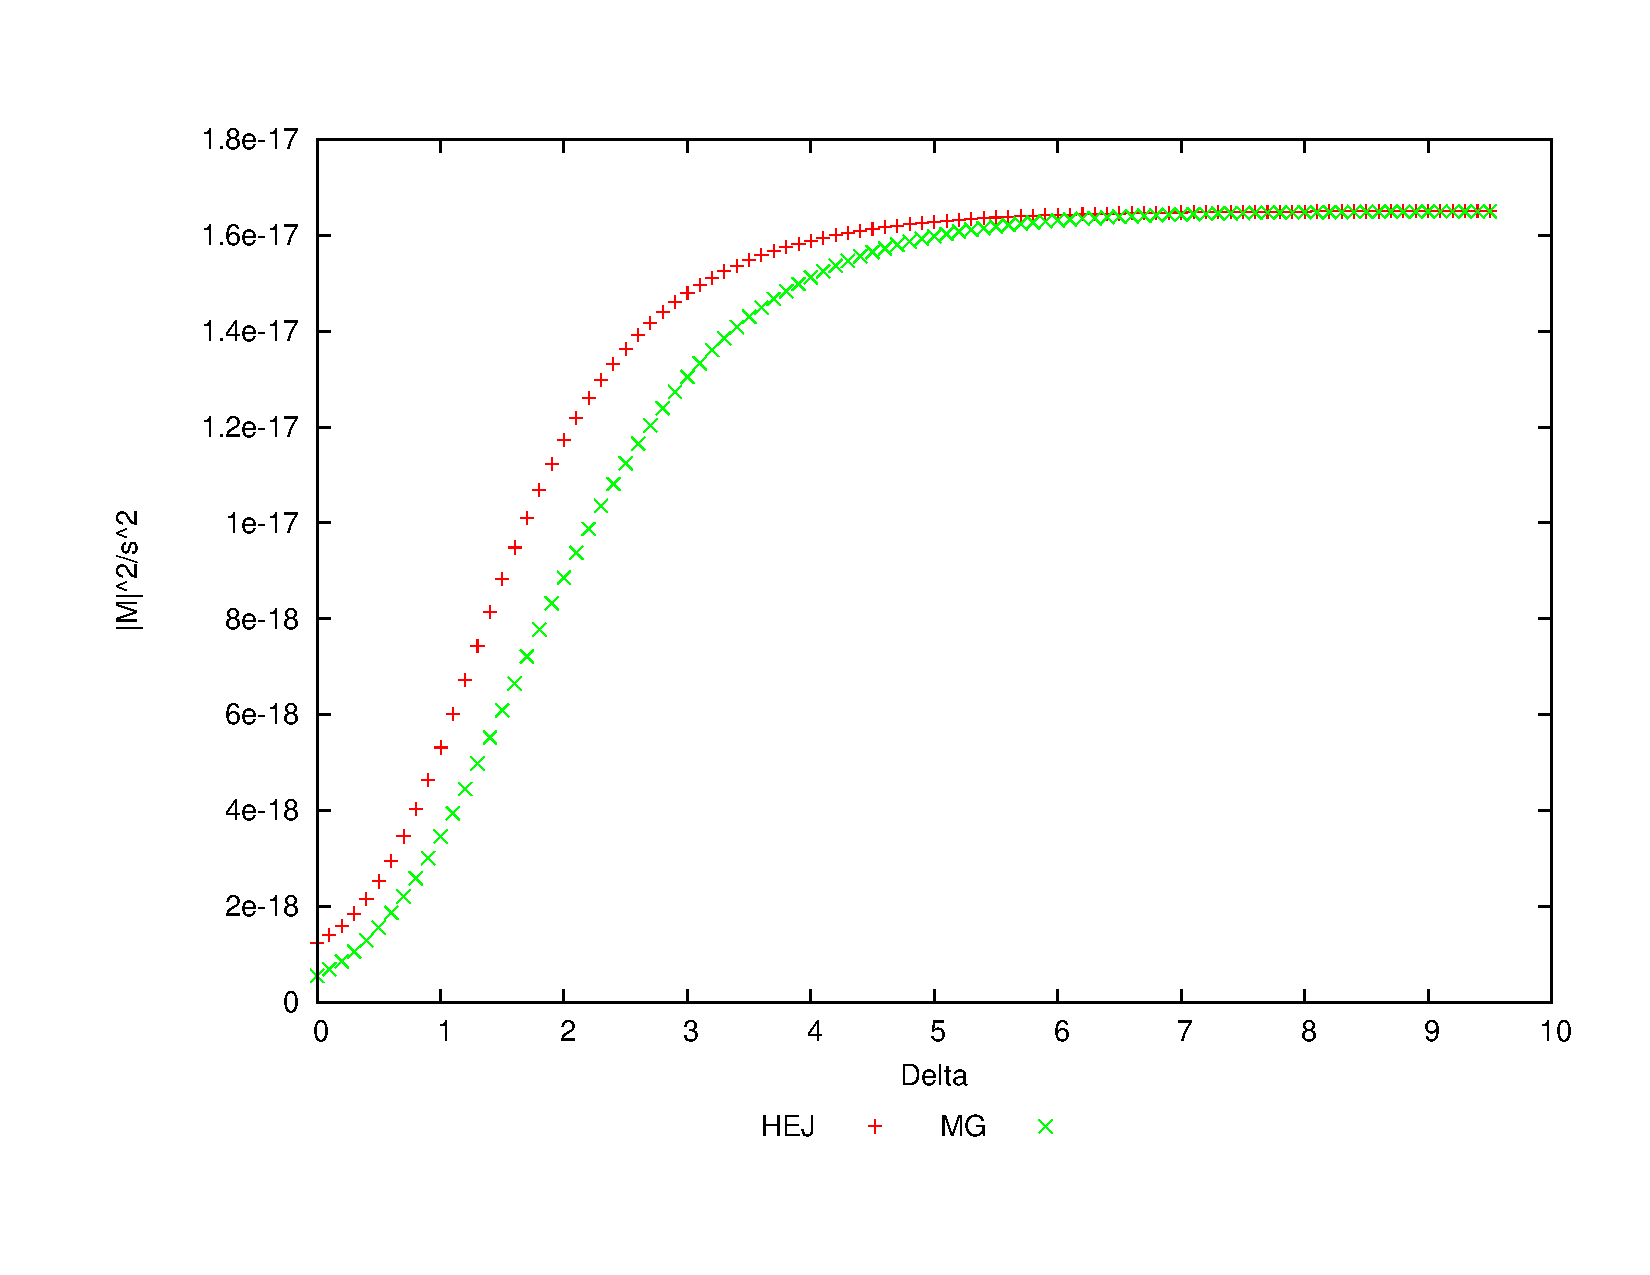
\includegraphics[scale=0.5]{Images/ug_nextfor.pdf}
\caption{Comparison between the HEJ effective vertex and the full LO result of the $gu \to Hggu$ amplitude for a forward H with an infinite top mass.}
\label{fig:ug_for} 
\end{figure}
%\todo{Swear this looked better before? Regenerate}

The agreement here is good across the phase space. Another slice of phase space we can take is one where all particles gradually move apart in rapidity;

\begin{subequations}
\begin{align}
p_1 &= (40 \cosh(\Delta),-40,0,40 \sinh(\Delta)), \\
p_H &= (\sqrt{40^2+m_H^2} \cosh(\Delta/3), 0,-40,\sqrt{40^2+m_H^2}  \sinh(\Delta/3)), \\
p_2 &= (40 \cosh(-\Delta/3),0,40,40 \sinh(-\Delta/3)), \\
p_3 &= (40 \cosh(-\Delta),40,0,40 \sinh(-\Delta)).
\end{align}
\end{subequations}

\begin{figure}[t]
\centering
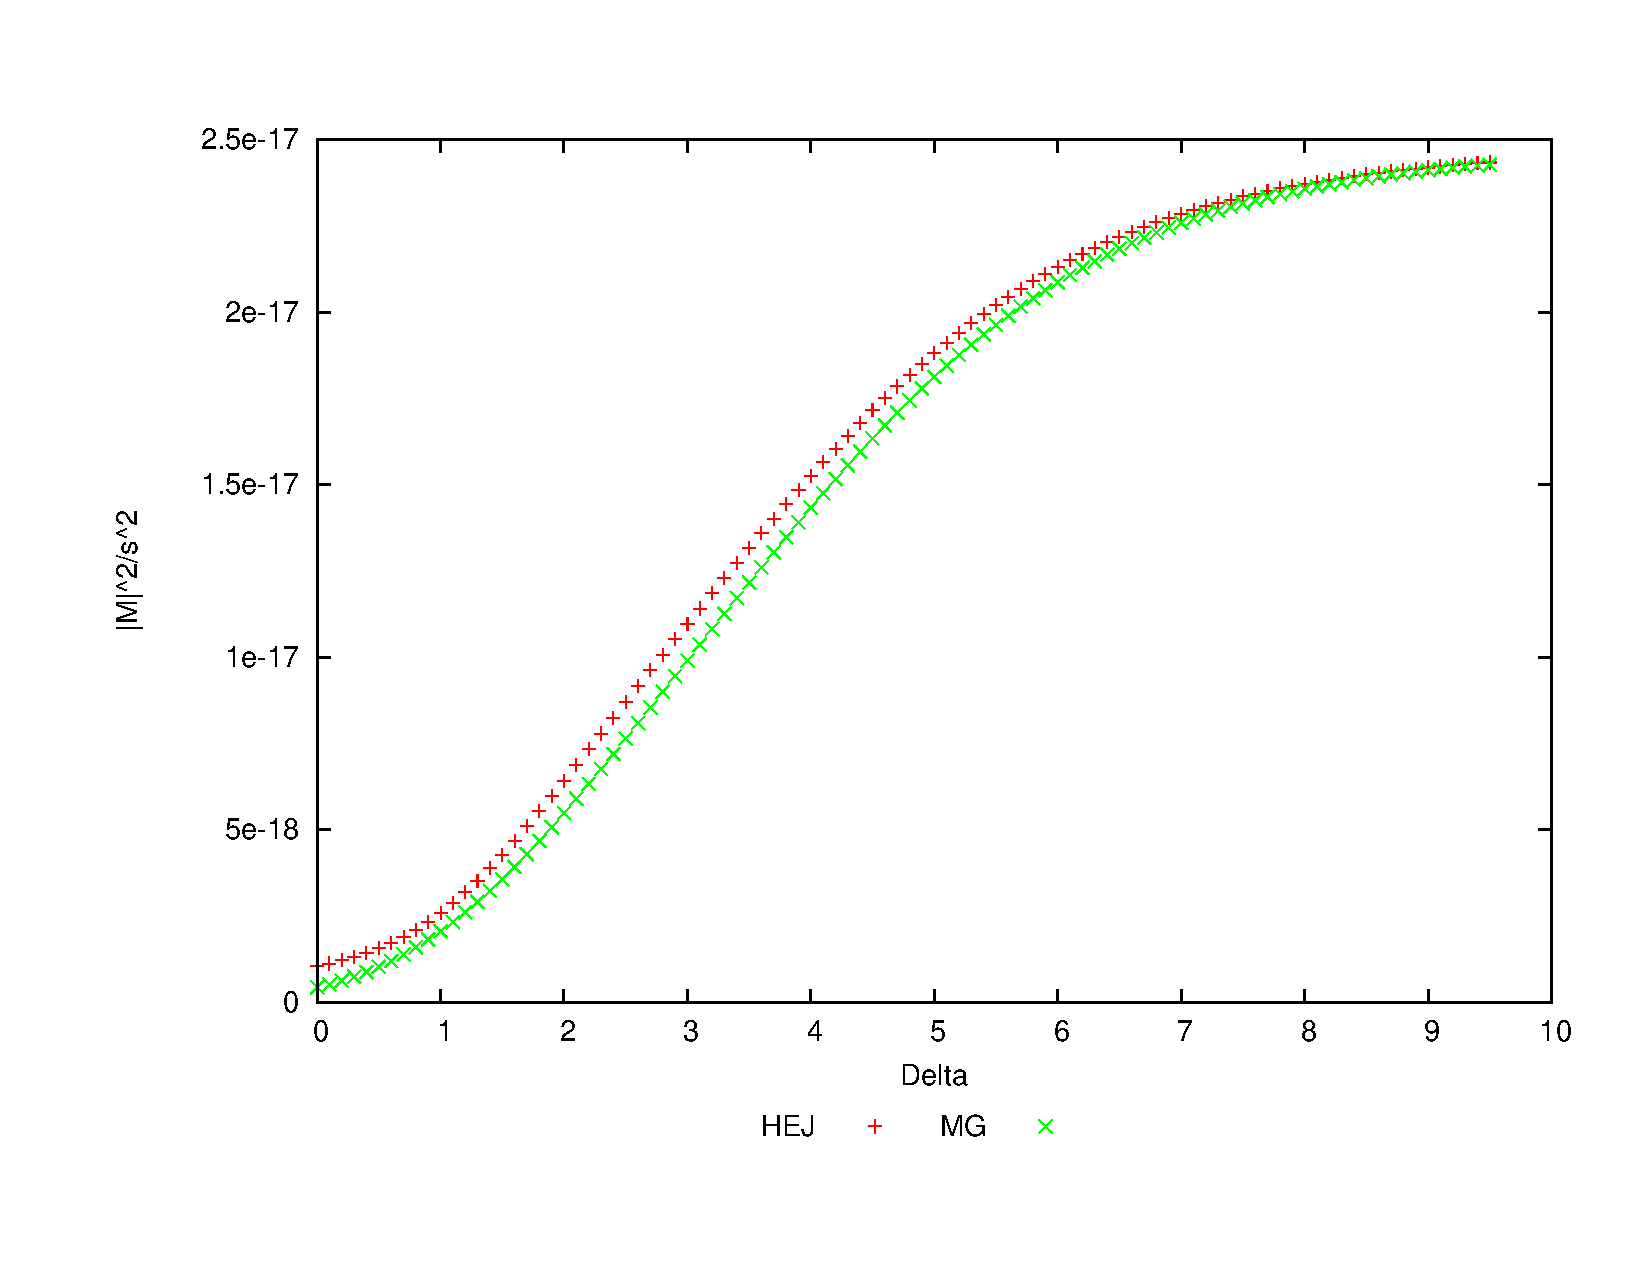
\includegraphics[scale=0.5]{/Users/jcockburn/FO_SVN/ug_cen.pdf}
\caption{Comparison between the HEJ effective vertex and the full LO result of the $gu \to gHgu$ amplitude for a central H with an infinite top mass.}
\label{fig:ug_cen}
\end{figure}


The explorer plot for this configuration is shown in figure \ref{fig:ug_cen}. Again, the agreement is good between the two lines. The other configuration to check is the one where the Higgs is more behind the extra emission. This contribution is not there for the $qg$ incoming state (at least, not with this matrix element) but is there for $gg$.  In that case, we can send $p_z \to -p_z$ in $p_2$ and $p_H$ in our momenta sets to probe this matrix element. In figures \ref{fig:gg_ggh_1}, \ref{fig:gg_ggh_2}, \ref{fig:gg_ggh_3} and \ref{fig:gg_ggh_4}, we show $gg \to Hggg$ with the Higgs being more forward, central but more forward than the extra emission, central but more backward than the extra emission and more backward respectively. All plots show agreement in the large $\Delta$ region, as expected, and track the LO result fairly well over the entire range. Confident in our forms for the matrix elements, we can move on to implementing them within the HEJ program and investigating their behaviour over the whole range of integrated phase space.

\begin{figure}[t]
\centering
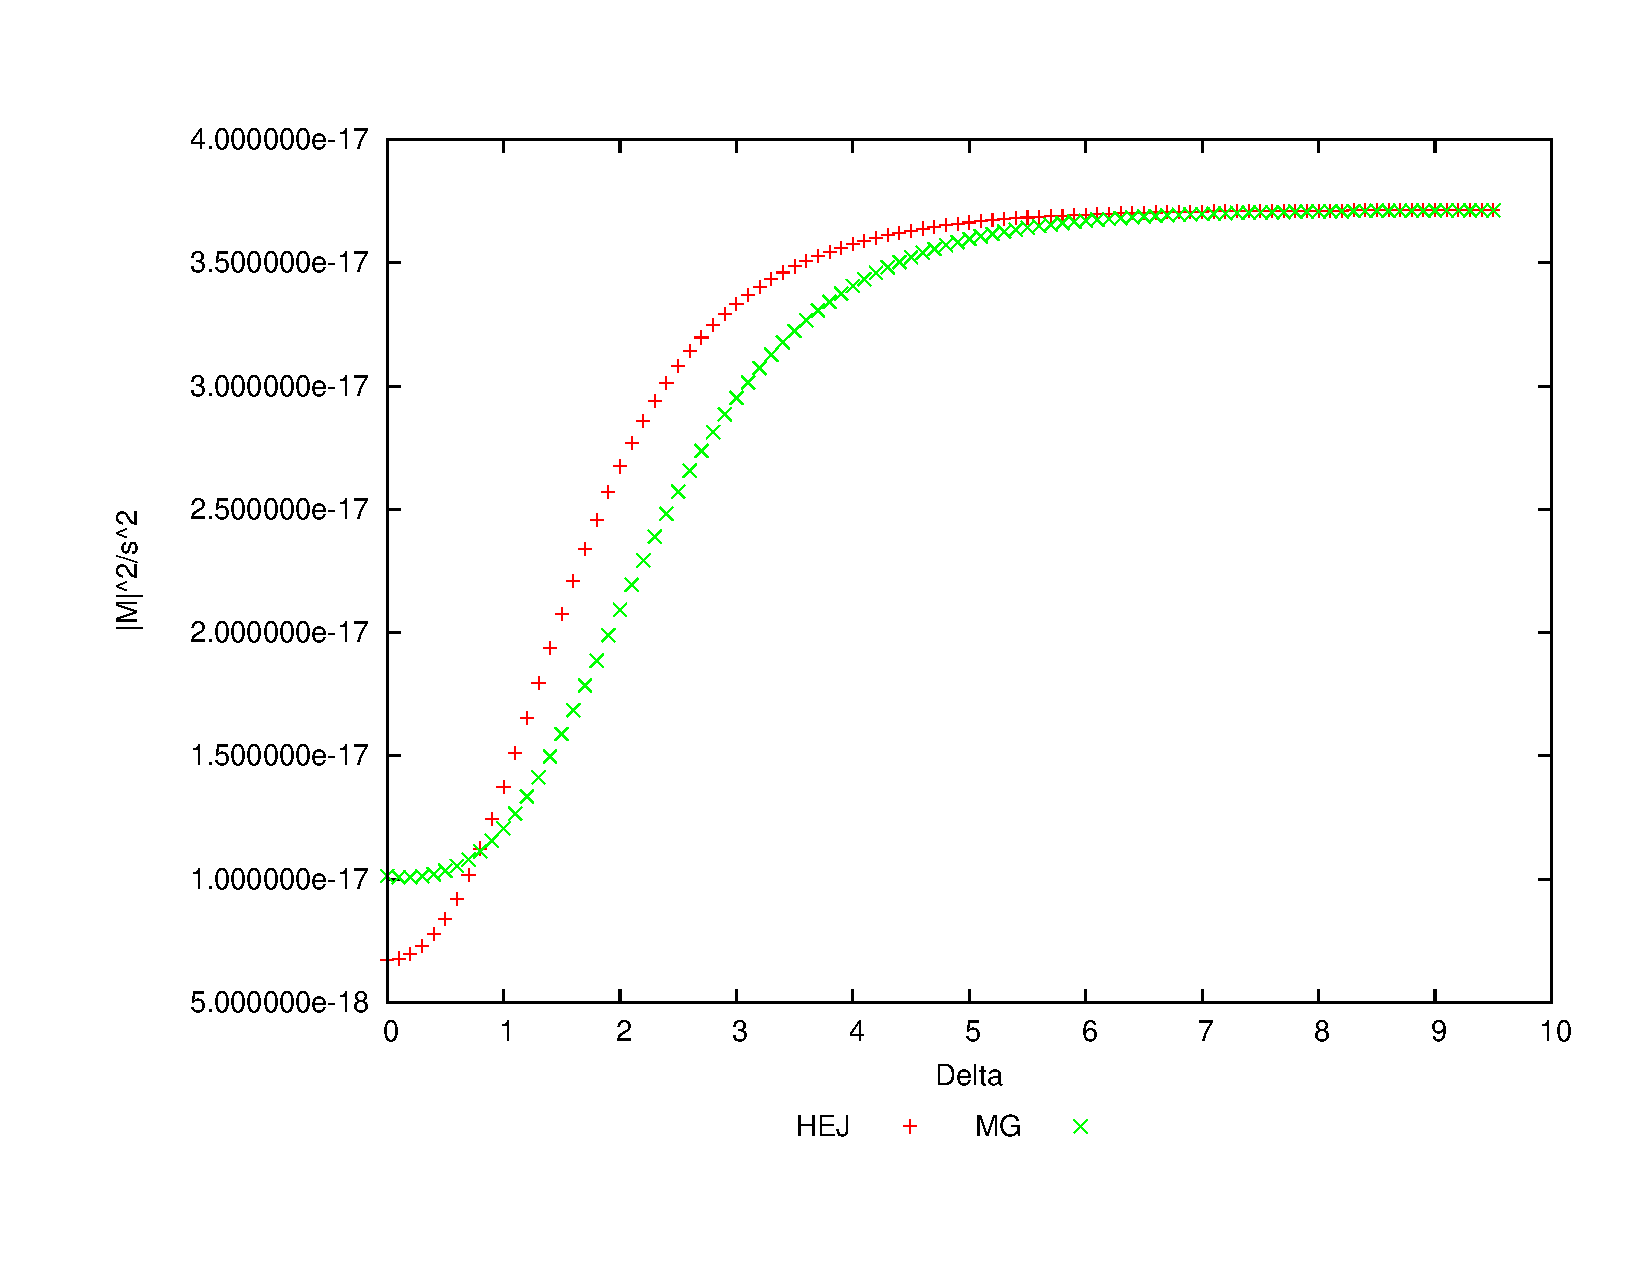
\includegraphics[scale=0.47]{Images/gg_nextfor.pdf}
\caption{Comparison between the HEJ effective vertex and the full LO result of the $gg \to Hggg$ amplitude for a forward H with an infinite top mass.}
\label{fig:gg_ggh_1}
\end{figure}

\begin{figure}[H]
\centering
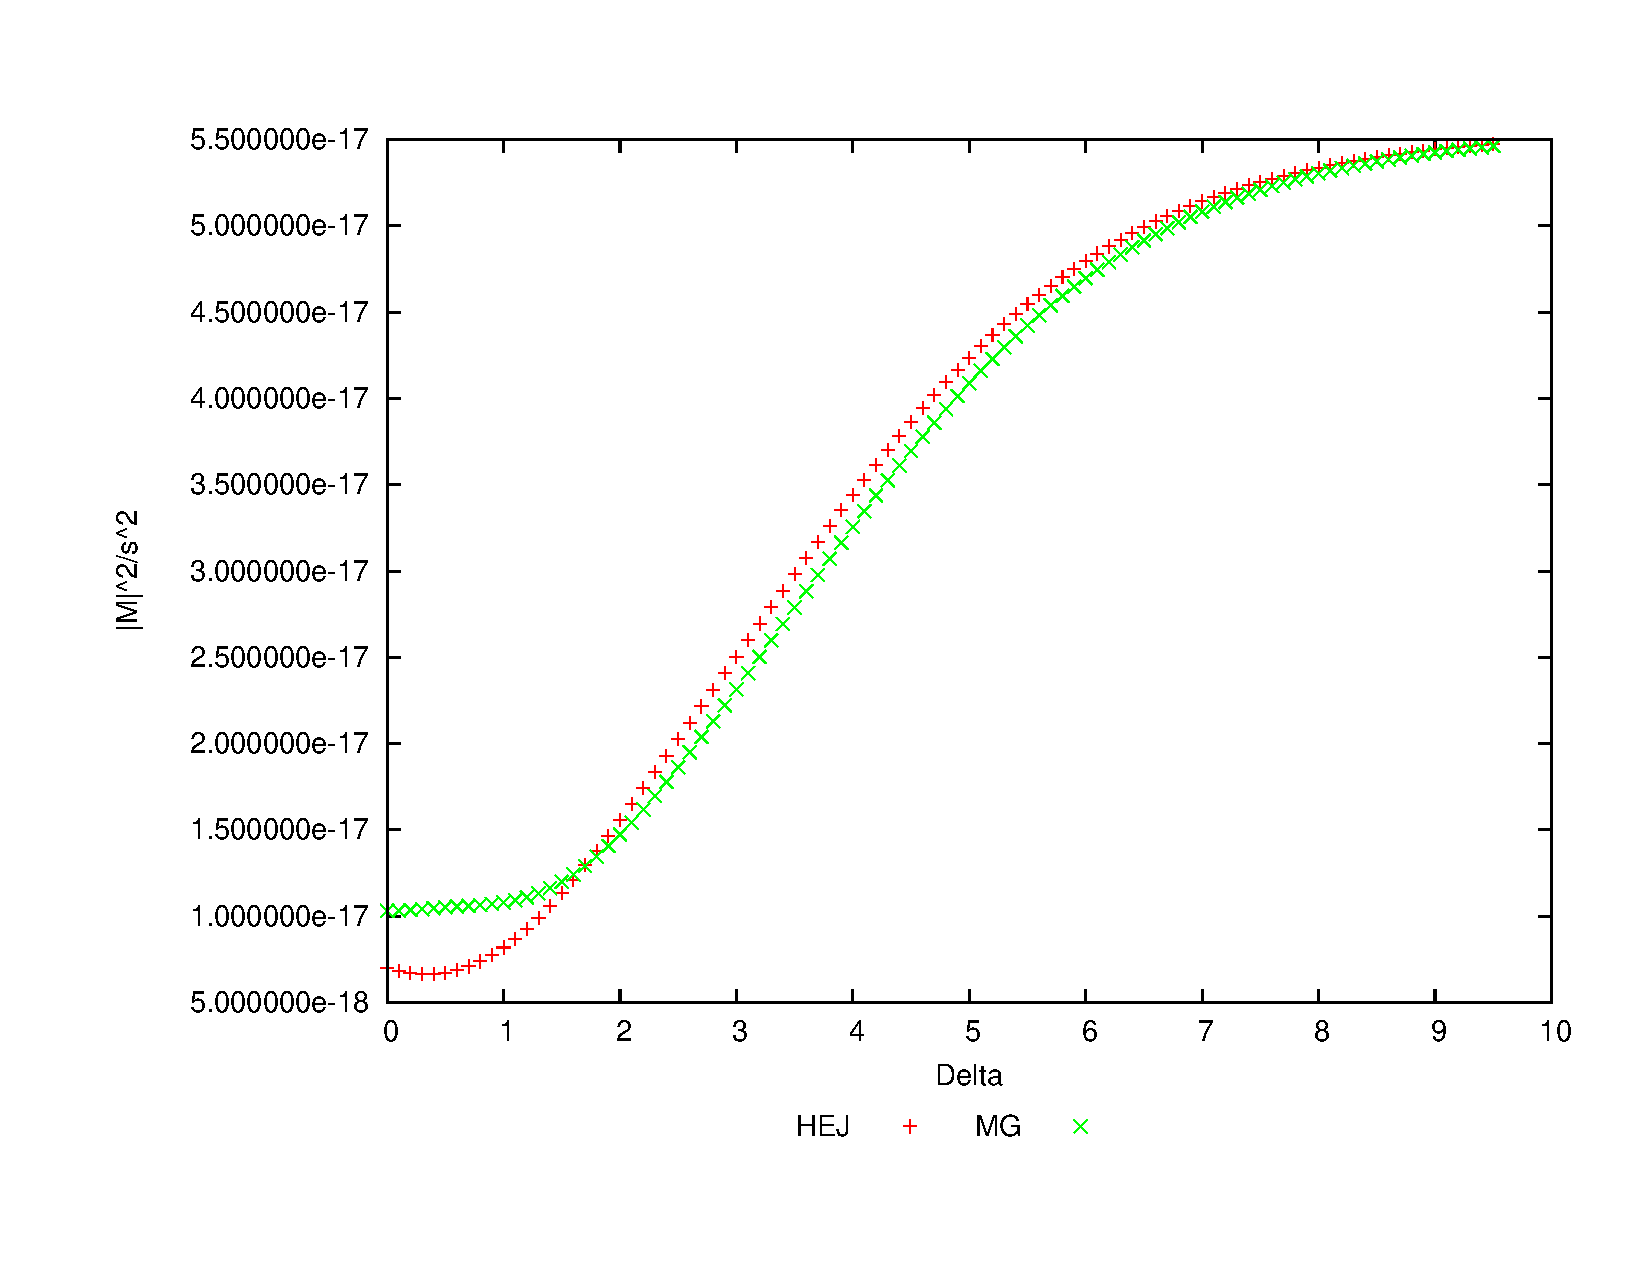
\includegraphics[scale=0.47]{Images/gg_cen1.pdf}
\caption{Comparison between the HEJ effective vertex and the full LO result of the $gg \to gHgg$ amplitude for a central H next to the extremal forward parton with an infinite top mass.}
\label{fig:gg_ggh_2}
\end{figure}

\begin{figure}[H]
\centering
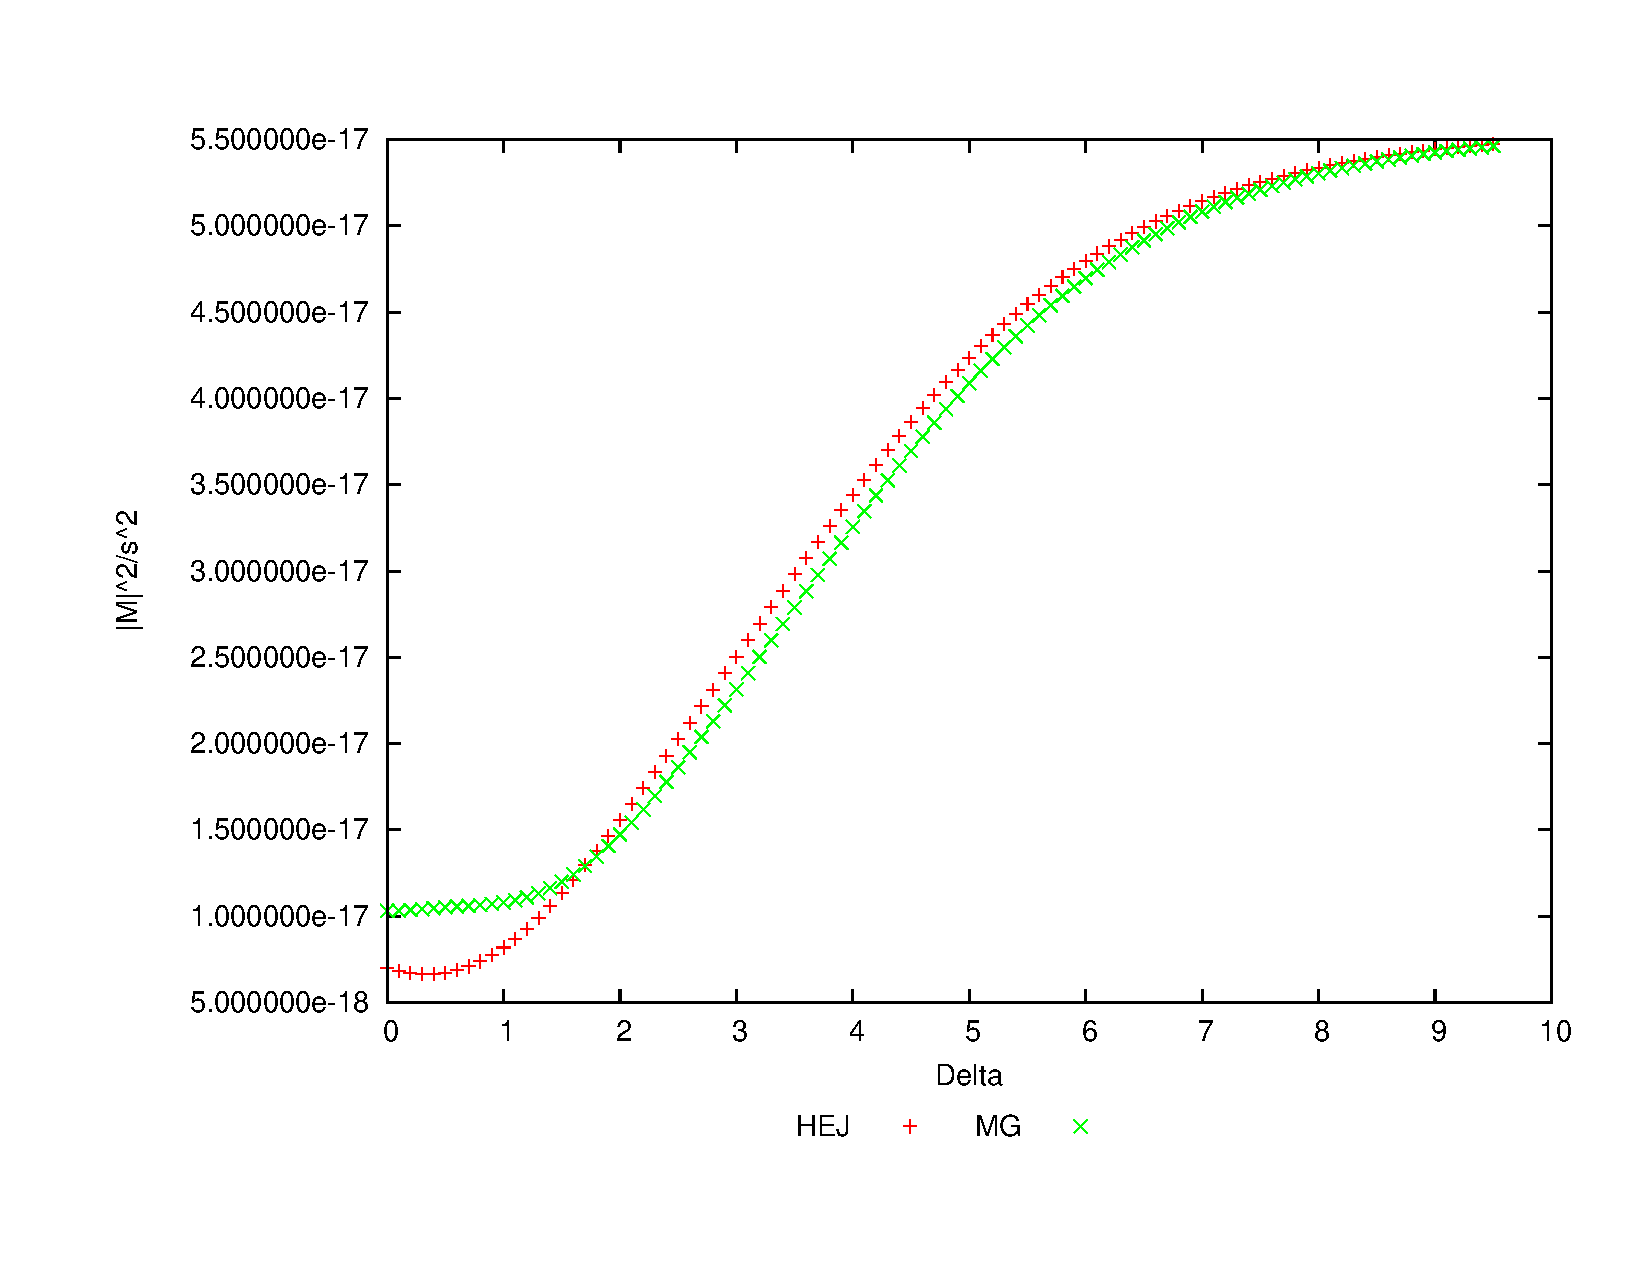
\includegraphics[scale=0.43]{Images/gg_cen2.pdf}
\caption{Comparison between the HEJ effective vertex and the full LO result of the $gg \to ggHg$ amplitude for a central H next to the extremal backward parton with an infinite top mass.}
\label{fig:gg_ggh_3}
\end{figure}


\begin{figure}[H]
\centering
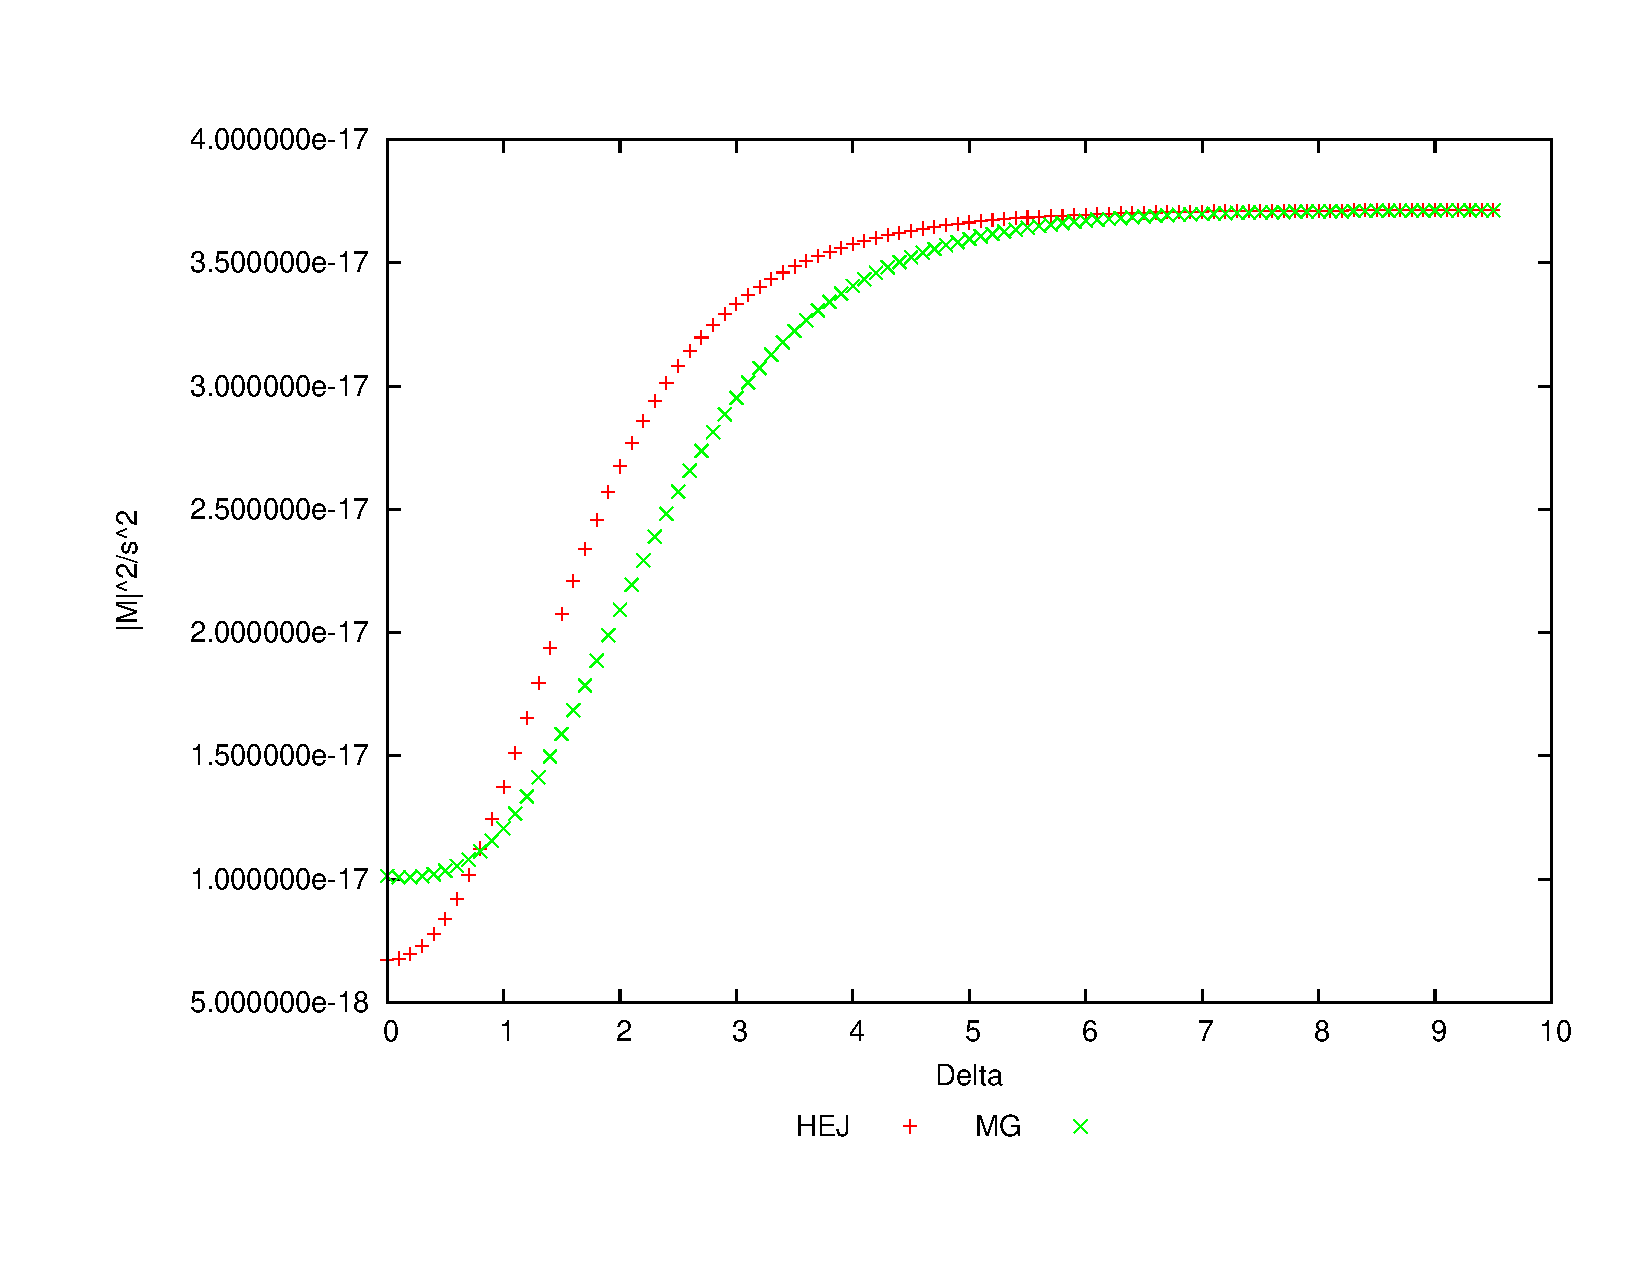
\includegraphics[scale=0.43]{Images/gg_nextback.pdf}
\caption{Comparison between the HEJ effective vertex and the full LO result of the $gg \to gggH$ amplitude for a backward H with an infinite top mass.}
\label{fig:gg_ggh_4}
\end{figure}

\section{Computational Aspects}

The addition of this new amplitude into the HEJ program is a much simpler task than it was for the NLL processes. Since we already had the amplitude in terms of the impact factors for the infinite top mass cases, the implementation was a case of adding the option to run with this finite top mass element instead. However, in order to calculate the scalar integrals in this amplitude, a HEJ interface to LoopTools is required. This is achieved in the program by setting a special instruction in the makefile; this way, if a user is not interested in using HEJ to generate for these types of events, they do not have to have LoopTools on their system. On the other hand, with the setting of a few library paths and setting the value for the special flag, LoopTools is quickly and simply added to the program such that running these new amplitudes can be done `out of the box'. \\
\\
Another consideration is how to implement the matching for the finite top mass case. It was decided that, given the length of time it would take to evaluate the matrix element with the full top mass included (especially in the three jet case) that it would not be wise to do the matching in this manner. Instead, since the infinite top mass elements are much quicker to evaluate, the matching is done by applying the finite top mass limit to the HEJ amplitude and dividing that by the full LO result in the effective theory. This yields an acceptable compromise, however it would clearly be ideal to match to the full result if the amount of time needed to do so was significantly reduced. This one motivation behind the development of the `inverse HEJ' technique. Since there are many resummation processes that can map to one jet process, the idea is to instead generate the jet level matrix element and work backwards from that to generate many resummation points to evaluate; hence `inverse'. This will drastically reduce the amount of calls we would make to the full finite top mass LO element and thus allow us to include this matching. 
%\todo{Make this a bit meatier. Include matching only to inf. Inverse HEJ?}

\section{Results}
%\todo{Explorer plots, integrated plots, other interesting things to note. Last real section to do! Arggh!}

Our first analysis will be $gu \to guH$ run, where the gluon is fixed to be the forward moving particle and the $u$ quark is fixed to be moving backwards. The Higgs can then be more forward than the gluon, more backward than the quark or in between the two particles in rapidity. For the forward case, we will use the matrix element we just derived to describe the process. For the central case, we will use the reweighted $qQ$ amplitude. Although our new matrix element will get this case correct, the reason we do not use it here is in anticipation of our resummation technique. Because we resum $t$-channel gluons, it is important to have a system where we can always unambiguously define what those gluons will be (or, in other words, we must have a consistent `resummation region', which for us will be the rapidity space between the gluon and quark). With our new amplitude, we can only resum the gluon connecting the effective vertex to the quark line, but for the reweighted $qQ$ case, we can resum the gluon from the top quark line to the triangle loop in the middle of the diagram and then from the triangle loop down to the bottom quark line. Choosing which matrix element we use based on the rapidity of the Higgs makes it clear which resummation we will be doing. Finally, since we have not discussed the case where the Higgs is behind the outgoing quark, we will set this process to zero for the time being. In the full program, we will use the impact factor already in the program for a Higgs emitted close to a quark line. An interesting plot to look at is the Higgs $p_T$ spectra. The infinite top mass limit should not do well at high values of Higgs $p_T$ as discussed in \cite{Duca2003} because it breaks the idea of the top quark mass being the largest relevant scale. This distribution is shown in figure \ref{fig:higgs_pt}. We see what we expect; at large Higgs $p_T$, the results obtained with the effective theory and the theory with finite quark mass effects are very different. Another interesting distribution to look at is the rapidity difference between the gluon and the quark. One could expect that the presence of a large rapidity gap (and so a large dijet invariant mass) might break the infinite top mass limit, but \cite{Duca2003} showed this not to be the case. The distribution shown in figure \ref{fig:higgs_ydiff} agrees with their conclusion. 

\begin{figure}[t]
\centering
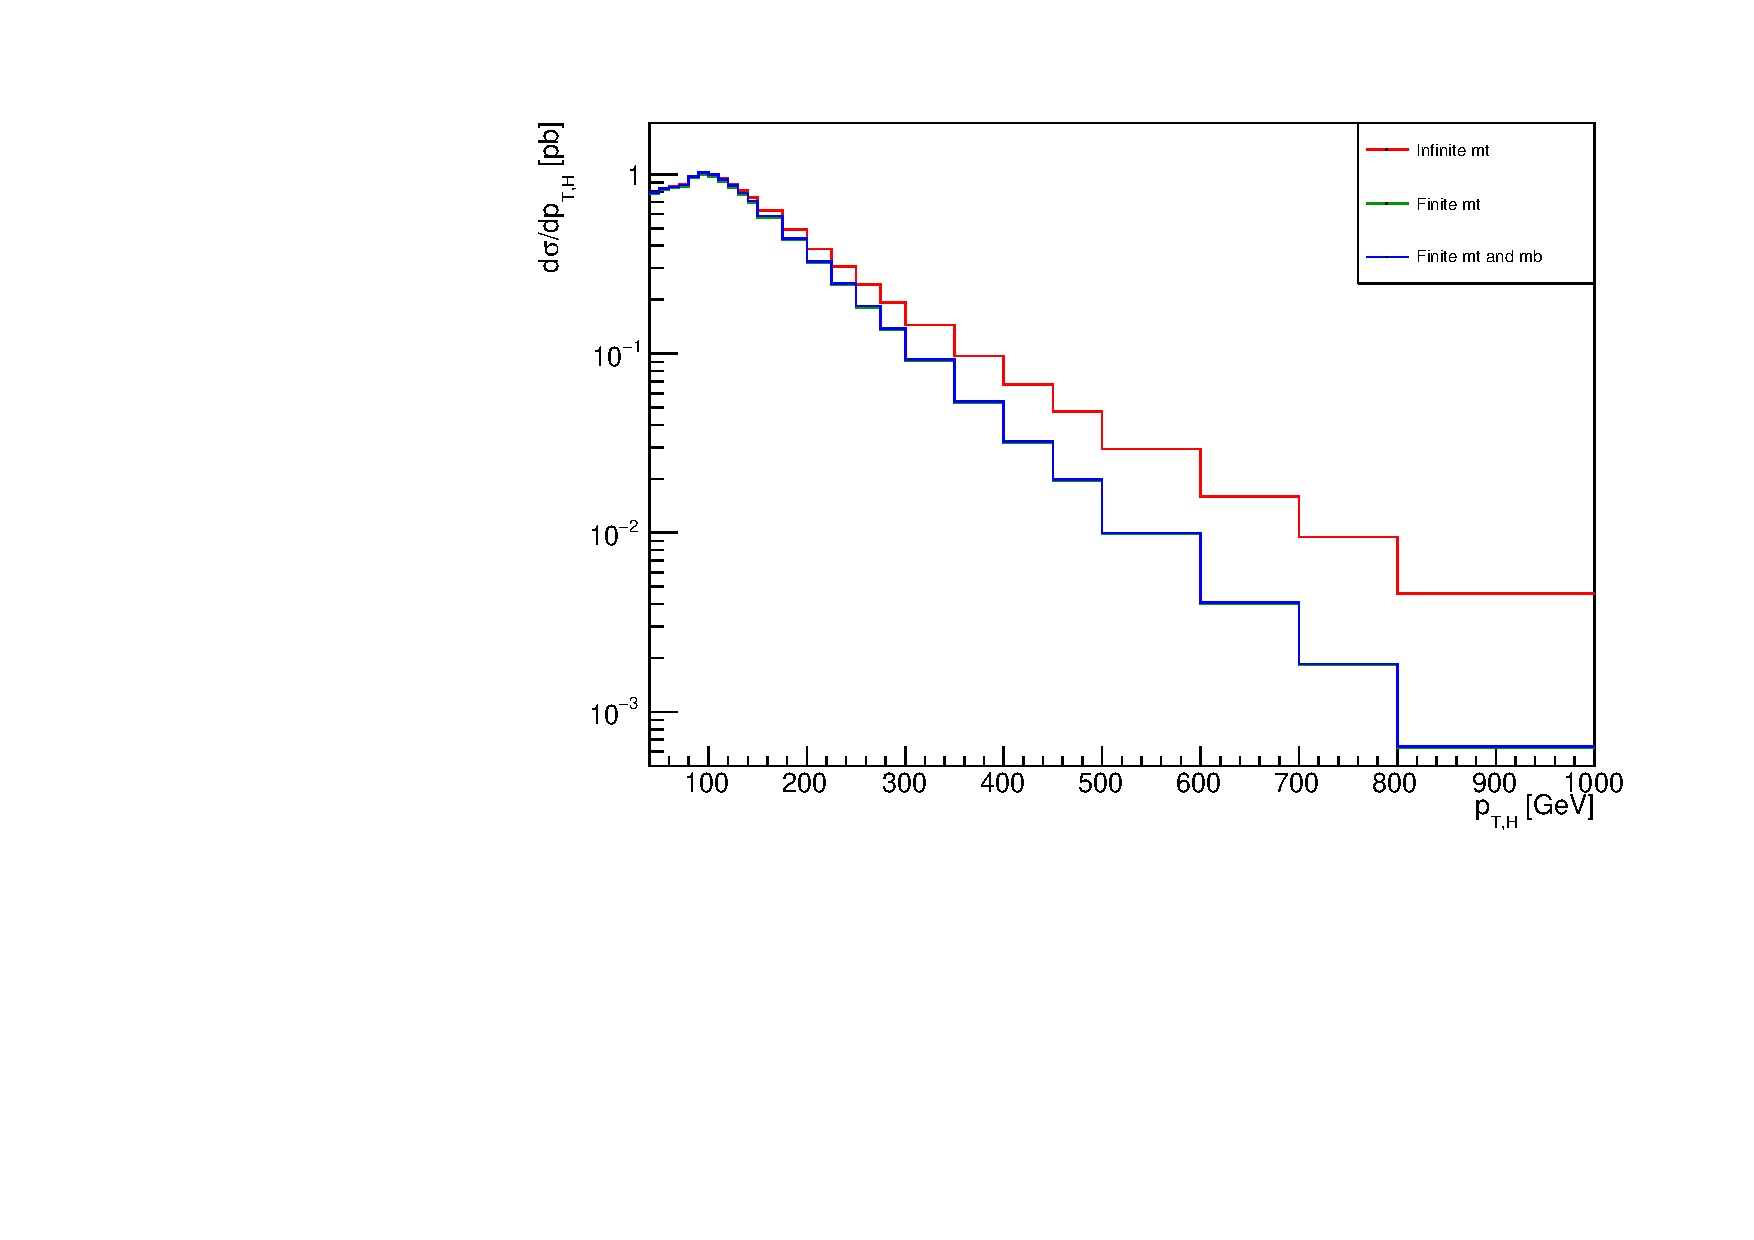
\includegraphics[scale=0.75]{Images/ptH_gu.pdf}
\caption{Comparison of infinite top mass, finite top mass and finite top + bottom mass cross sections in $gu \to guH$, binned in Higgs $p_T$ }
\label{fig:higgs_pt}
\end{figure}

\begin{figure}[H]
\centering
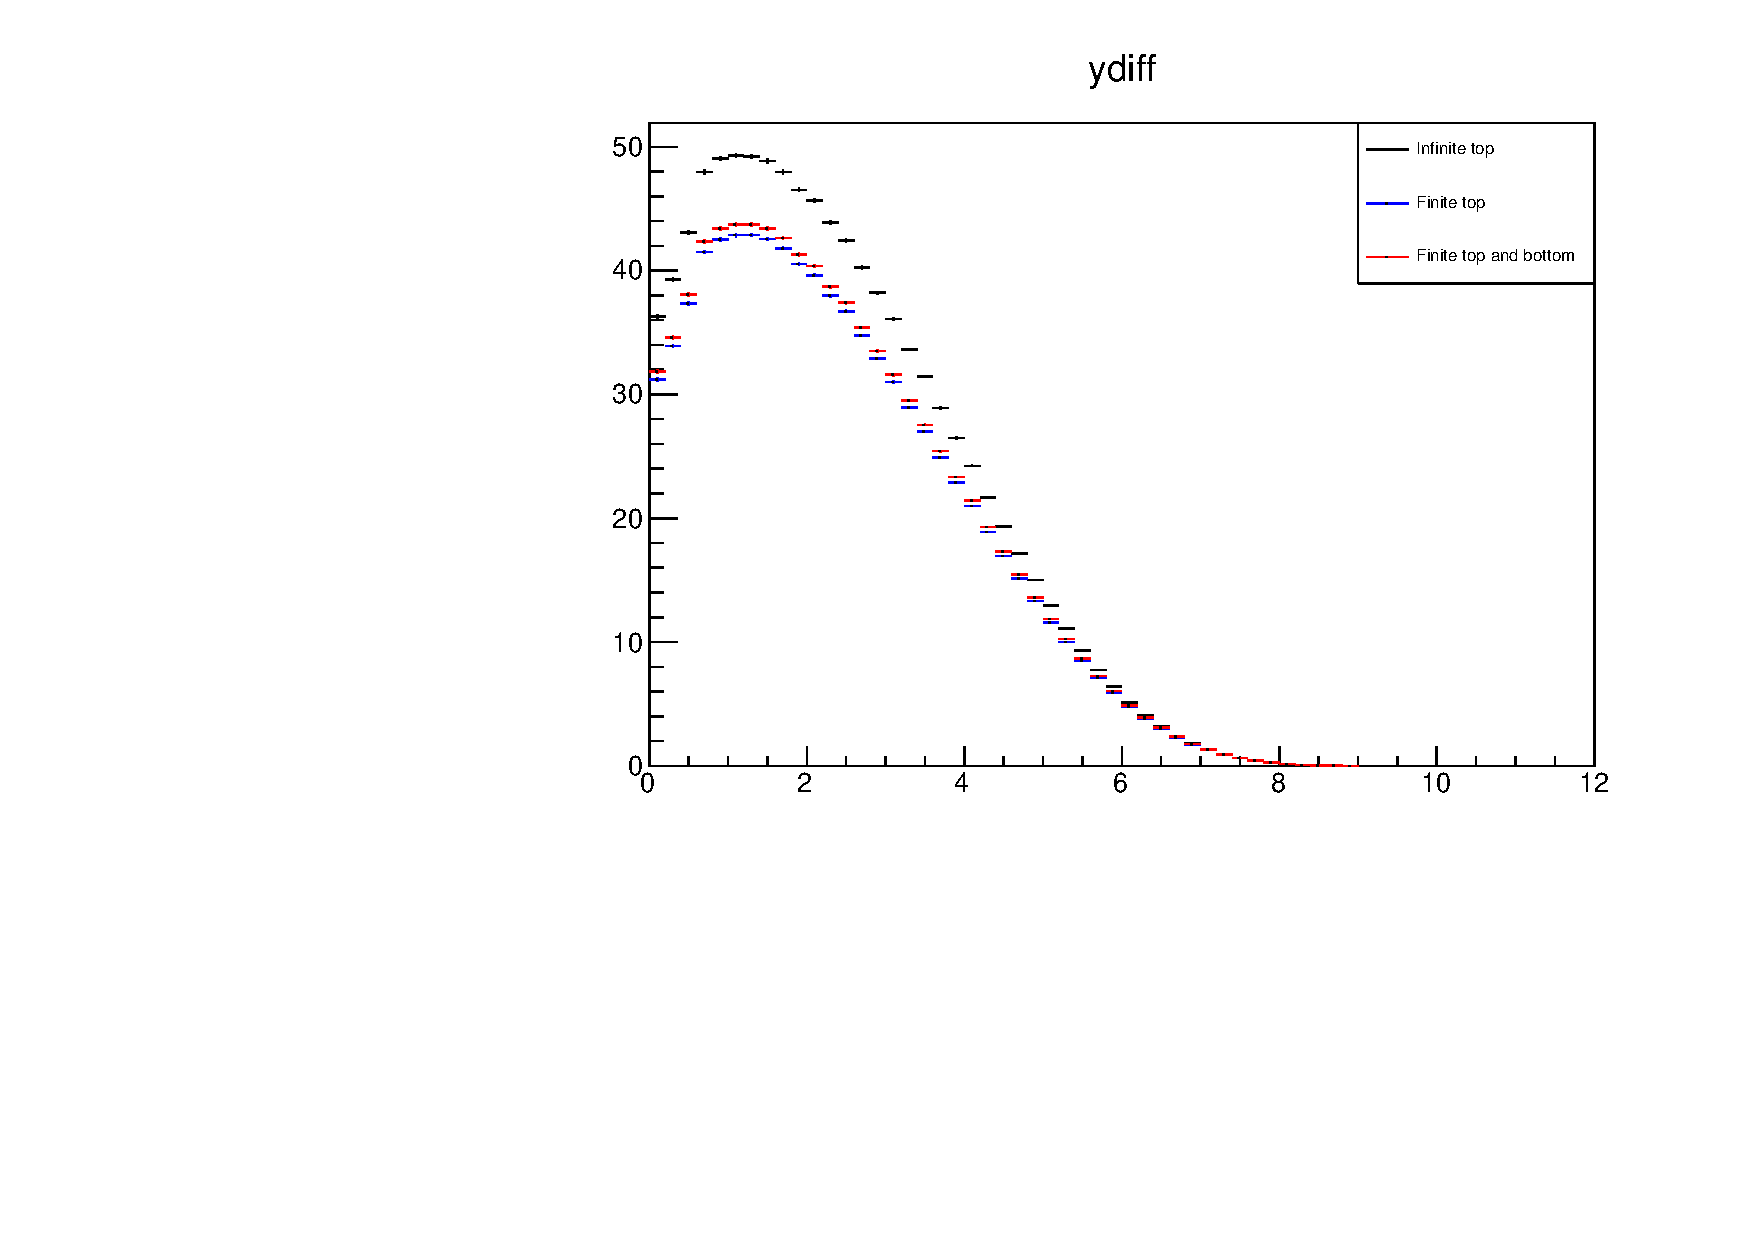
\includegraphics[scale=0.75]{Images/ydiff_gu.pdf}
\caption{Comparison of infinite top mass, finite top mass and finite top + bottom mass cross sections in $gu \to guH$, binned in rapidity difference between the gluon and up quark}
\label{fig:higgs_ydiff}
\end{figure}

We should also remember that, given kinematical constraints on the energy of the collider, the high $\Delta_y$ region must come with relatively low transverse scales, so it further lends support to the idea that the transverse scales are the defining ones in terms of how well the effective theory does. We can do the same analysis with a $gg$ incoming state, which in the high energy regime is just the $qg$ amplitude reweighted by a colour factor. In this case, the Higgs can be either forward of a forward moving gluon, backward of a backward moving one or in-between. We can describe all of these configurations; the first with our new amplitude, the latter with a reweighted $qQ$ amp and the second with our new matrix element as well so long as we account for phase differences in some calculations we did (all derived results were explicitly considering that the Higgs is emitted forward). If this is considered correctly, then the amount of cross section coming from a forward Higgs should be equal (up to statistical fluctuations) to that coming from a backward Higgs. We show that this is the case in figure \ref{fig:gg_crosssection}, where the green and blue lines are so close together to be essentially indistinguishable. The results for the Higgs $p_T$ and $\Delta y_{12}$ distributions are essentially the same as the $gq$ case and we present them here for completeness in figures \ref{fig:pth_gg} and \ref{fig:ydiff_gg}. 

\begin{figure}[t]
\centering
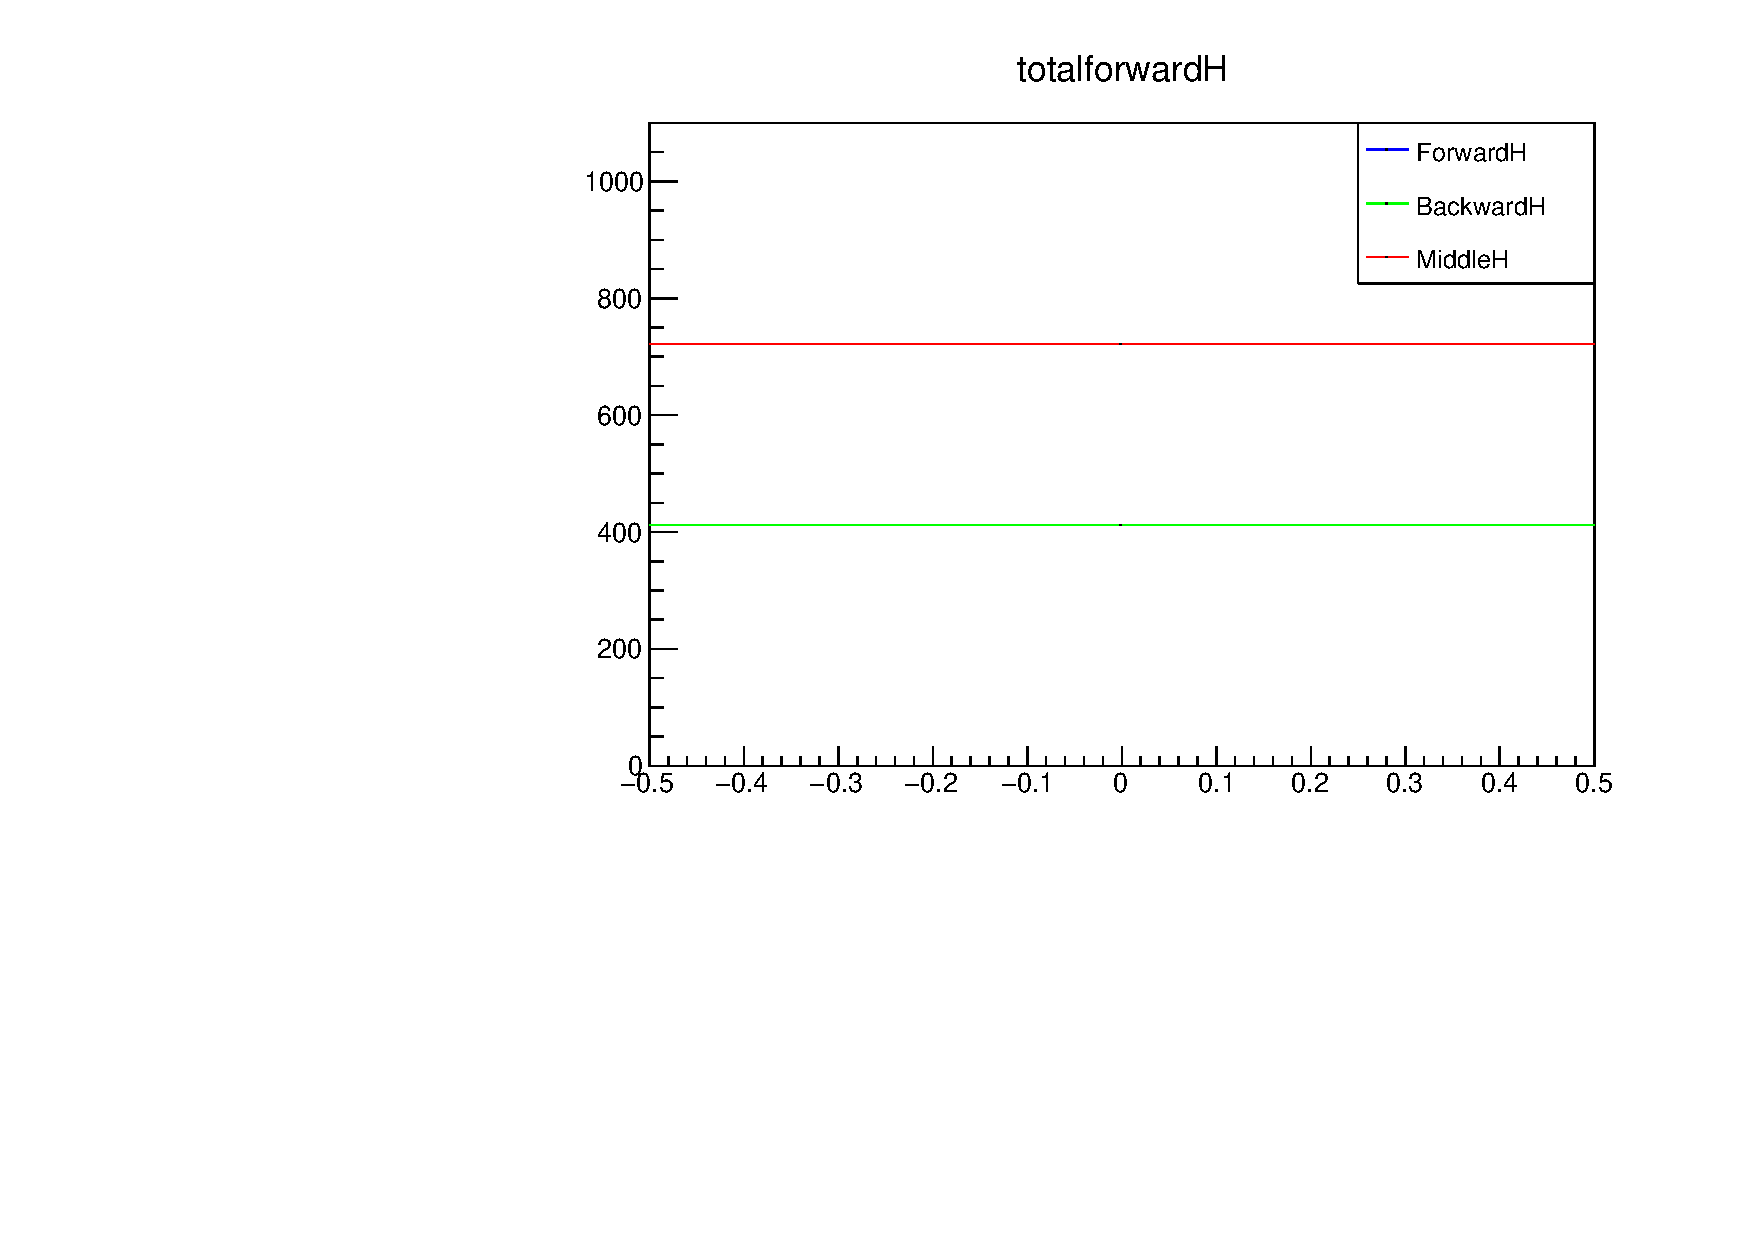
\includegraphics[scale=0.75]{Images/xsec_breakdown_ggh.pdf}
\caption{Cross section breakdown in $gg \to ggH$ into forward Higgs production. backward Higgs production and central Higgs with infinite top mass.}
\label{fig:gg_crosssection}
\end{figure}

\begin{figure}[H]
\centering
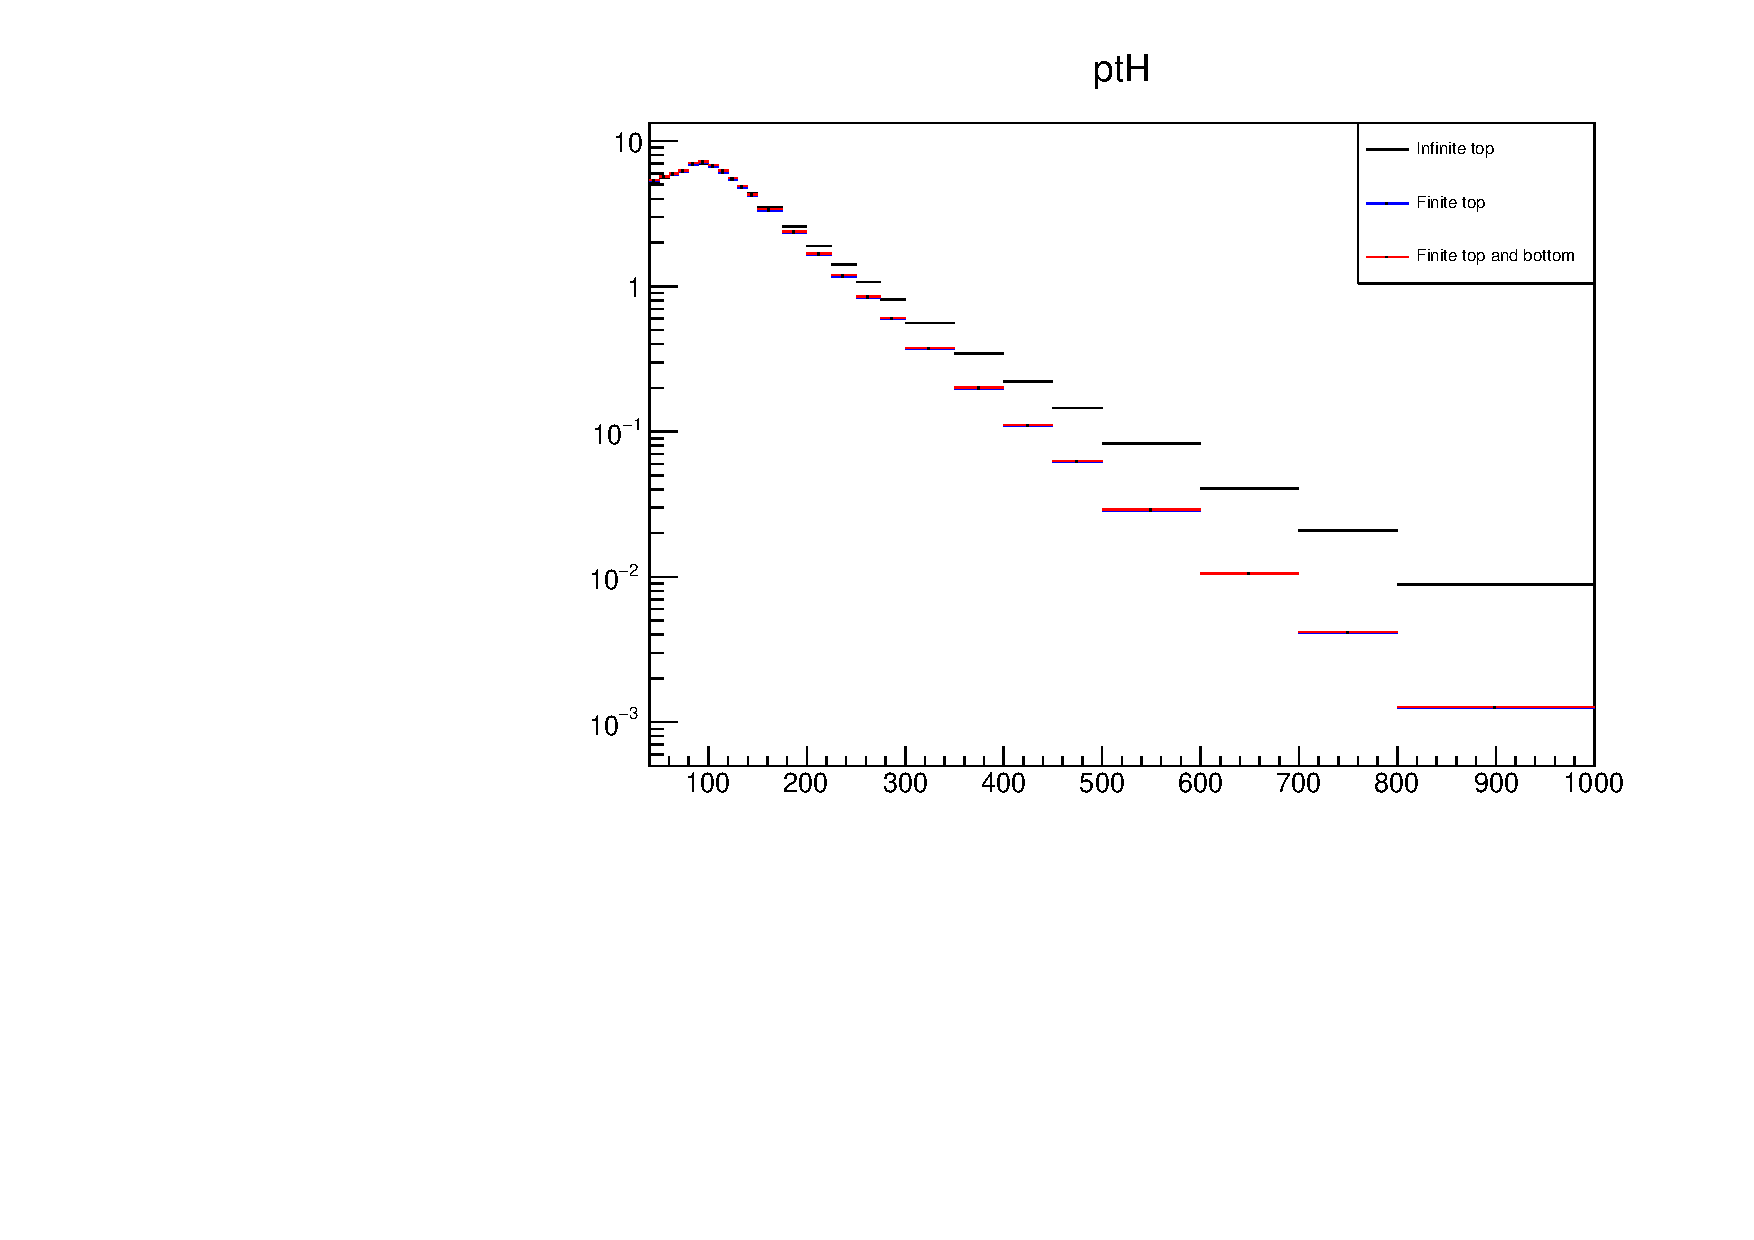
\includegraphics[scale=0.7]{Images/ptH_gg.pdf}
\caption{Comparison of infinite top mass, finite top mass and finite top + bottom mass cross sections in $gg \to ggH$, binned in Higgs $p_T$. }
\label{fig:pth_gg}
\end{figure}

\begin{figure}[H]
\centering
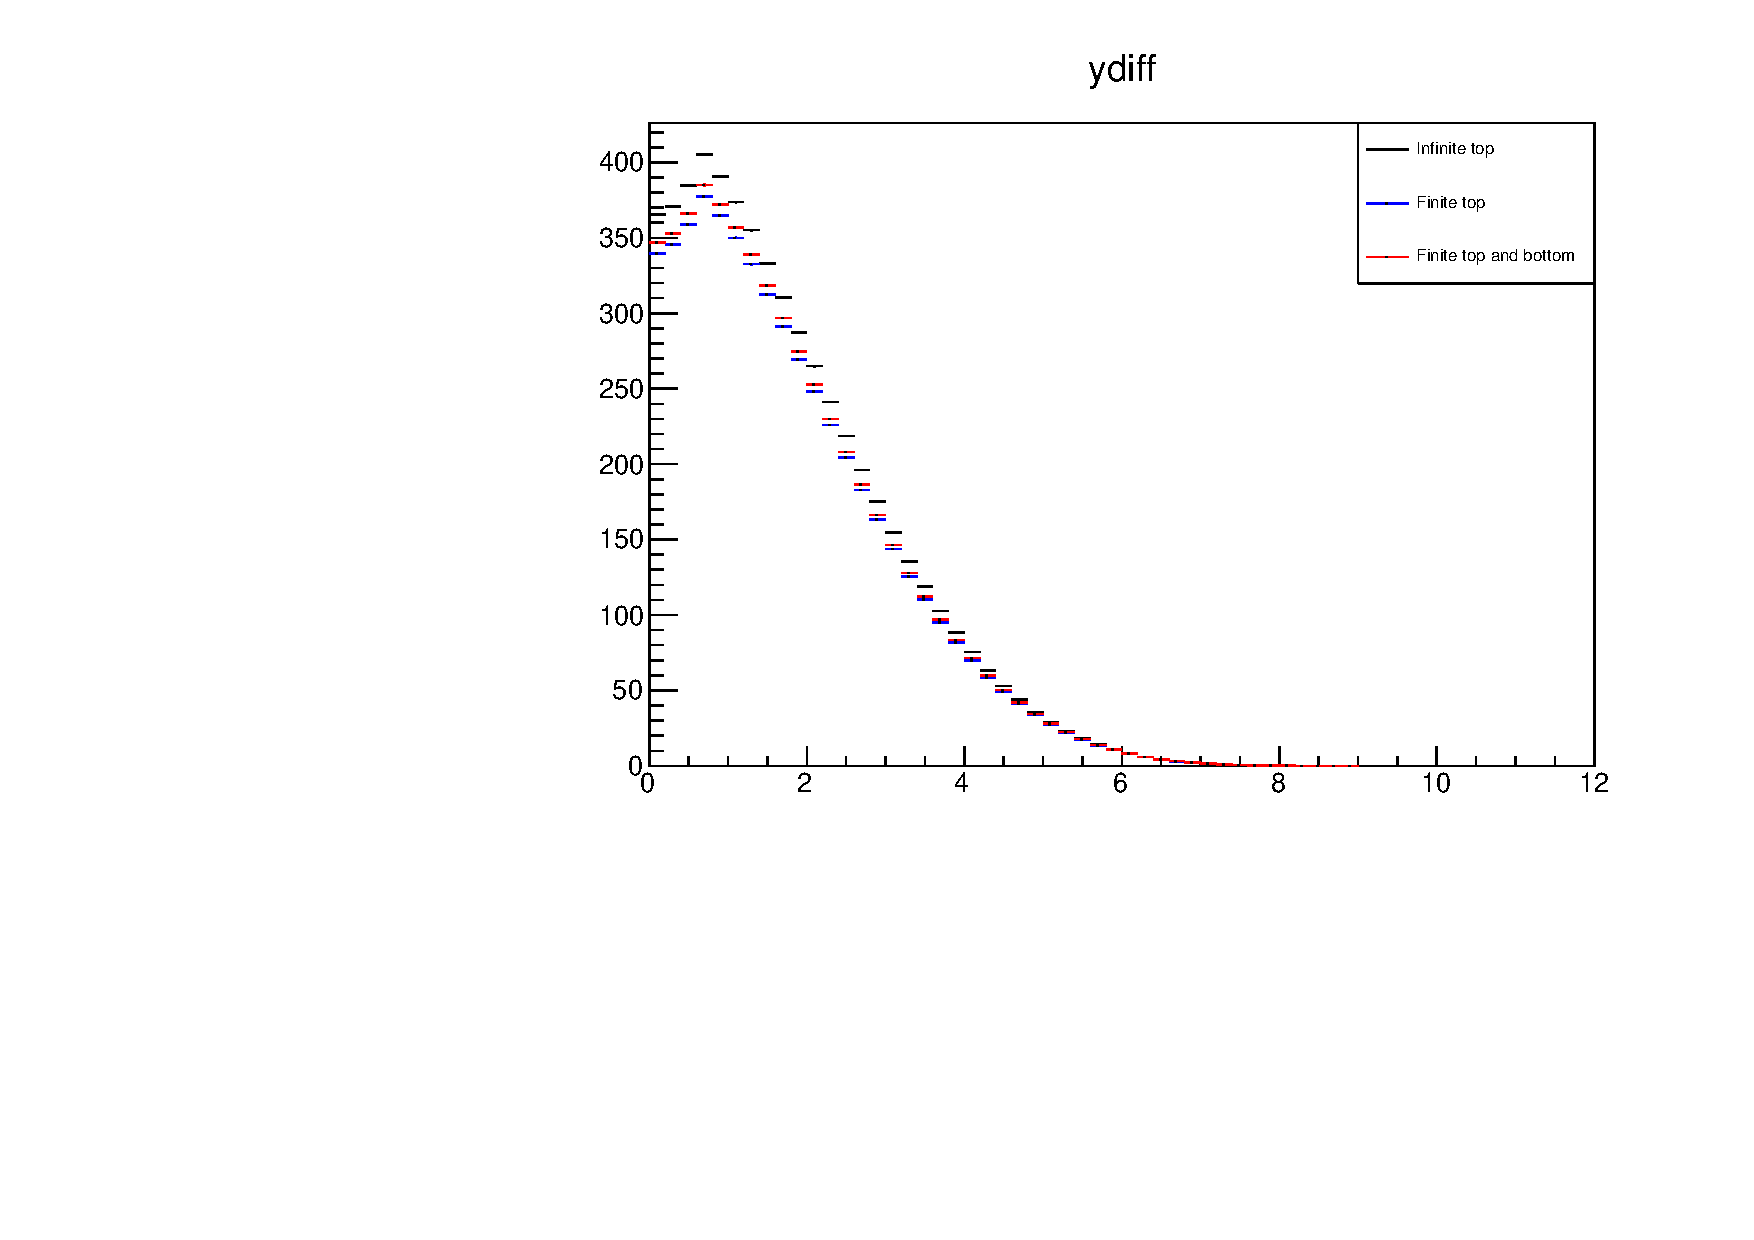
\includegraphics[scale=0.7]{Images/ydiff_gg.pdf}
\caption{Comparison of infinite top mass, finite top mass and finite top + bottom mass cross sections in $gg \to ggH$, binned in rapidity difference between the gluon and up quark.}
\label{fig:ydiff_gg}
\end{figure}
\todo{All analysis plots need labels on axes}
We also investigate the effect of adding a third jet so as to look at a $gg \to gggH$ analysis. An interesting plot to show is that again of the Higgs $p_T$ as shown in figure \ref{fig:pth_gg_gggH}. We see there is a significant difference between the infinite top mass results and the finite top mass results in all bins - strikingly, at low Higgs $p_T$. This would seem to contradict our prediction that low transverse scales lead mean that the effective theory is valid. The problem is that, in a three jet event, you can manufacture a situation whereby there is a large hierarchy between the transverse scales that enter the Higgs vertex. If instead we plot the cross section as a function of the largest transverse scale that enters into this vertex, we should then once more again see the agreement in the low $p_T$ end. Figure \ref{fig:maxprop} shows this clearly. %\todo{Run analysis with full pp to H}

\begin{figure}[t]
\centering
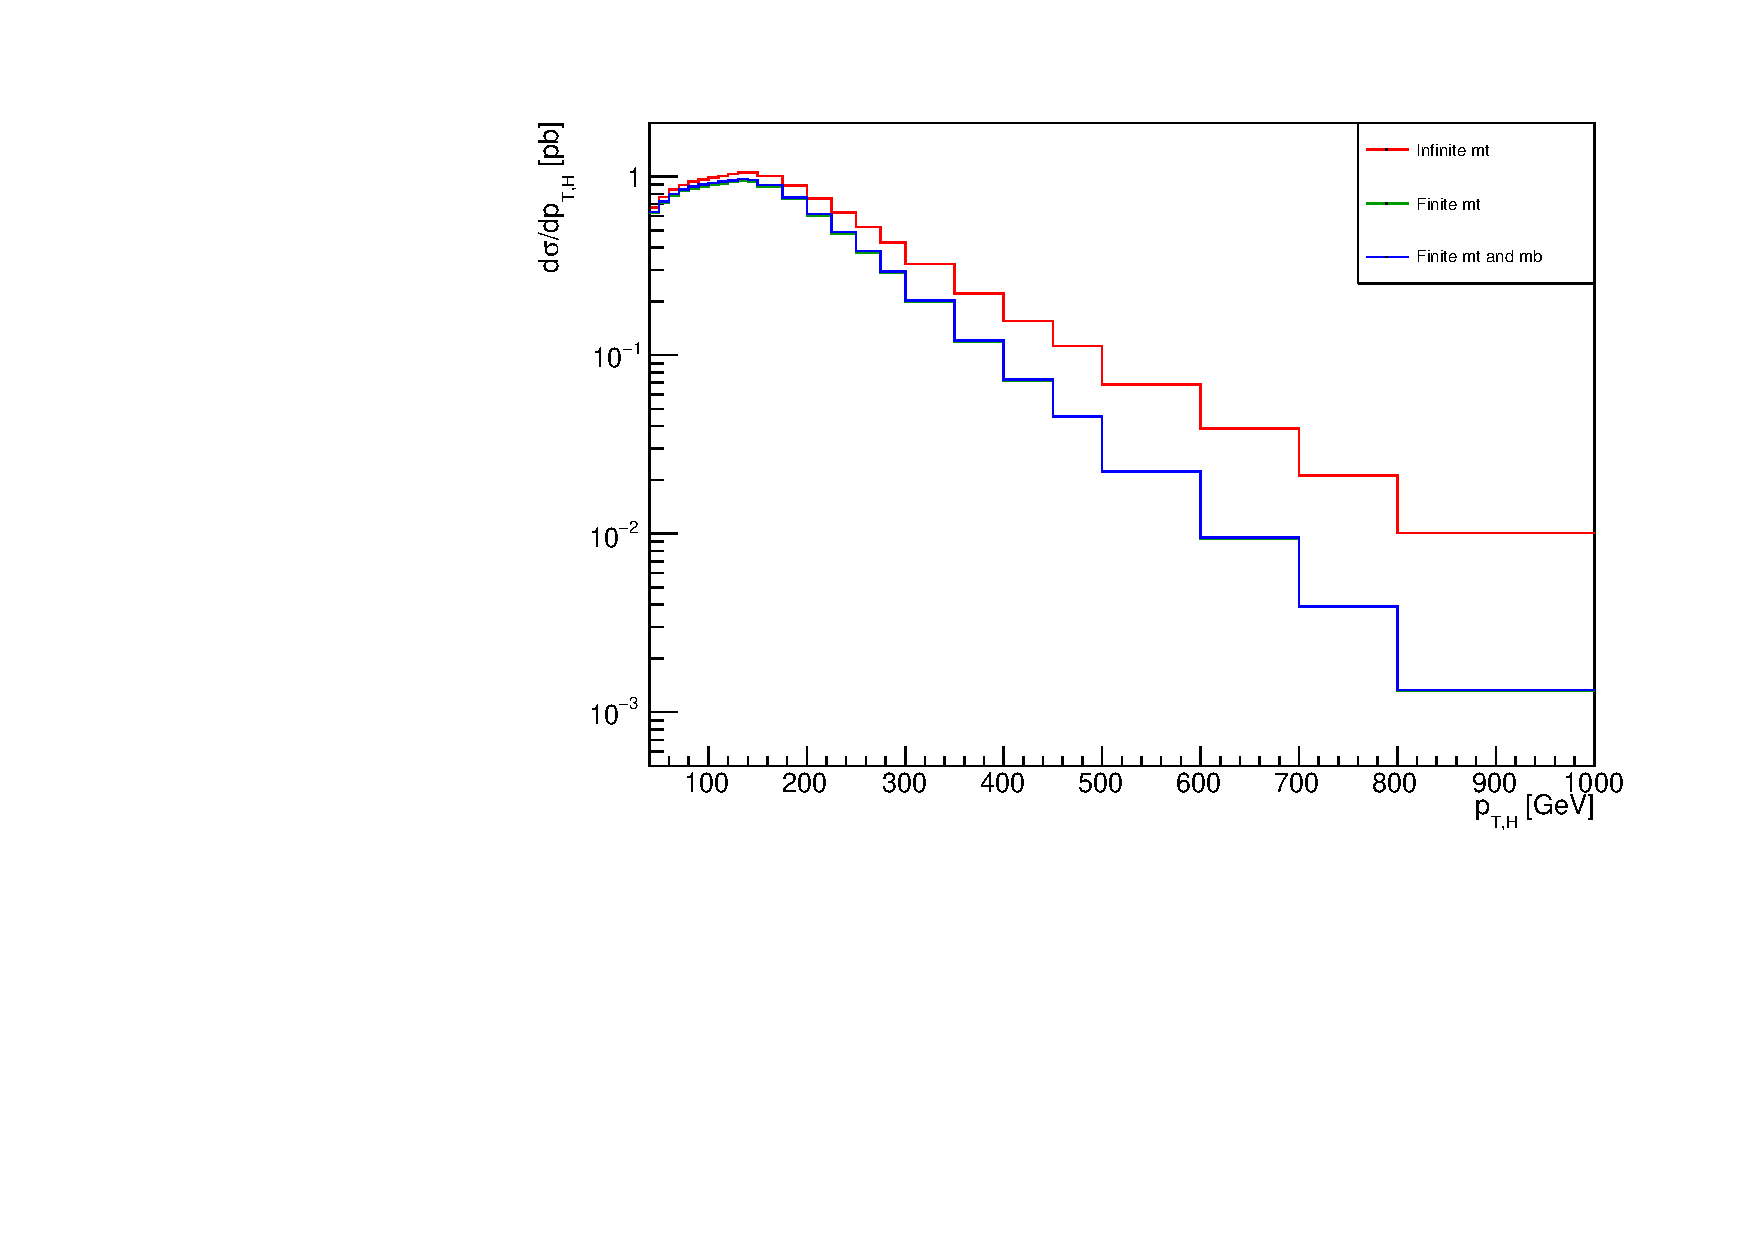
\includegraphics[scale=0.72]{Images/ptH_3j.pdf}
\caption{Comparison of infinite top mass, finite top mass and finite top + bottom mass cross sections in $gg \to gggH$, binned in Higgs $p_T$. }
\label{fig:pth_gg_gggH}
\end{figure}

\begin{figure}[t]
\centering
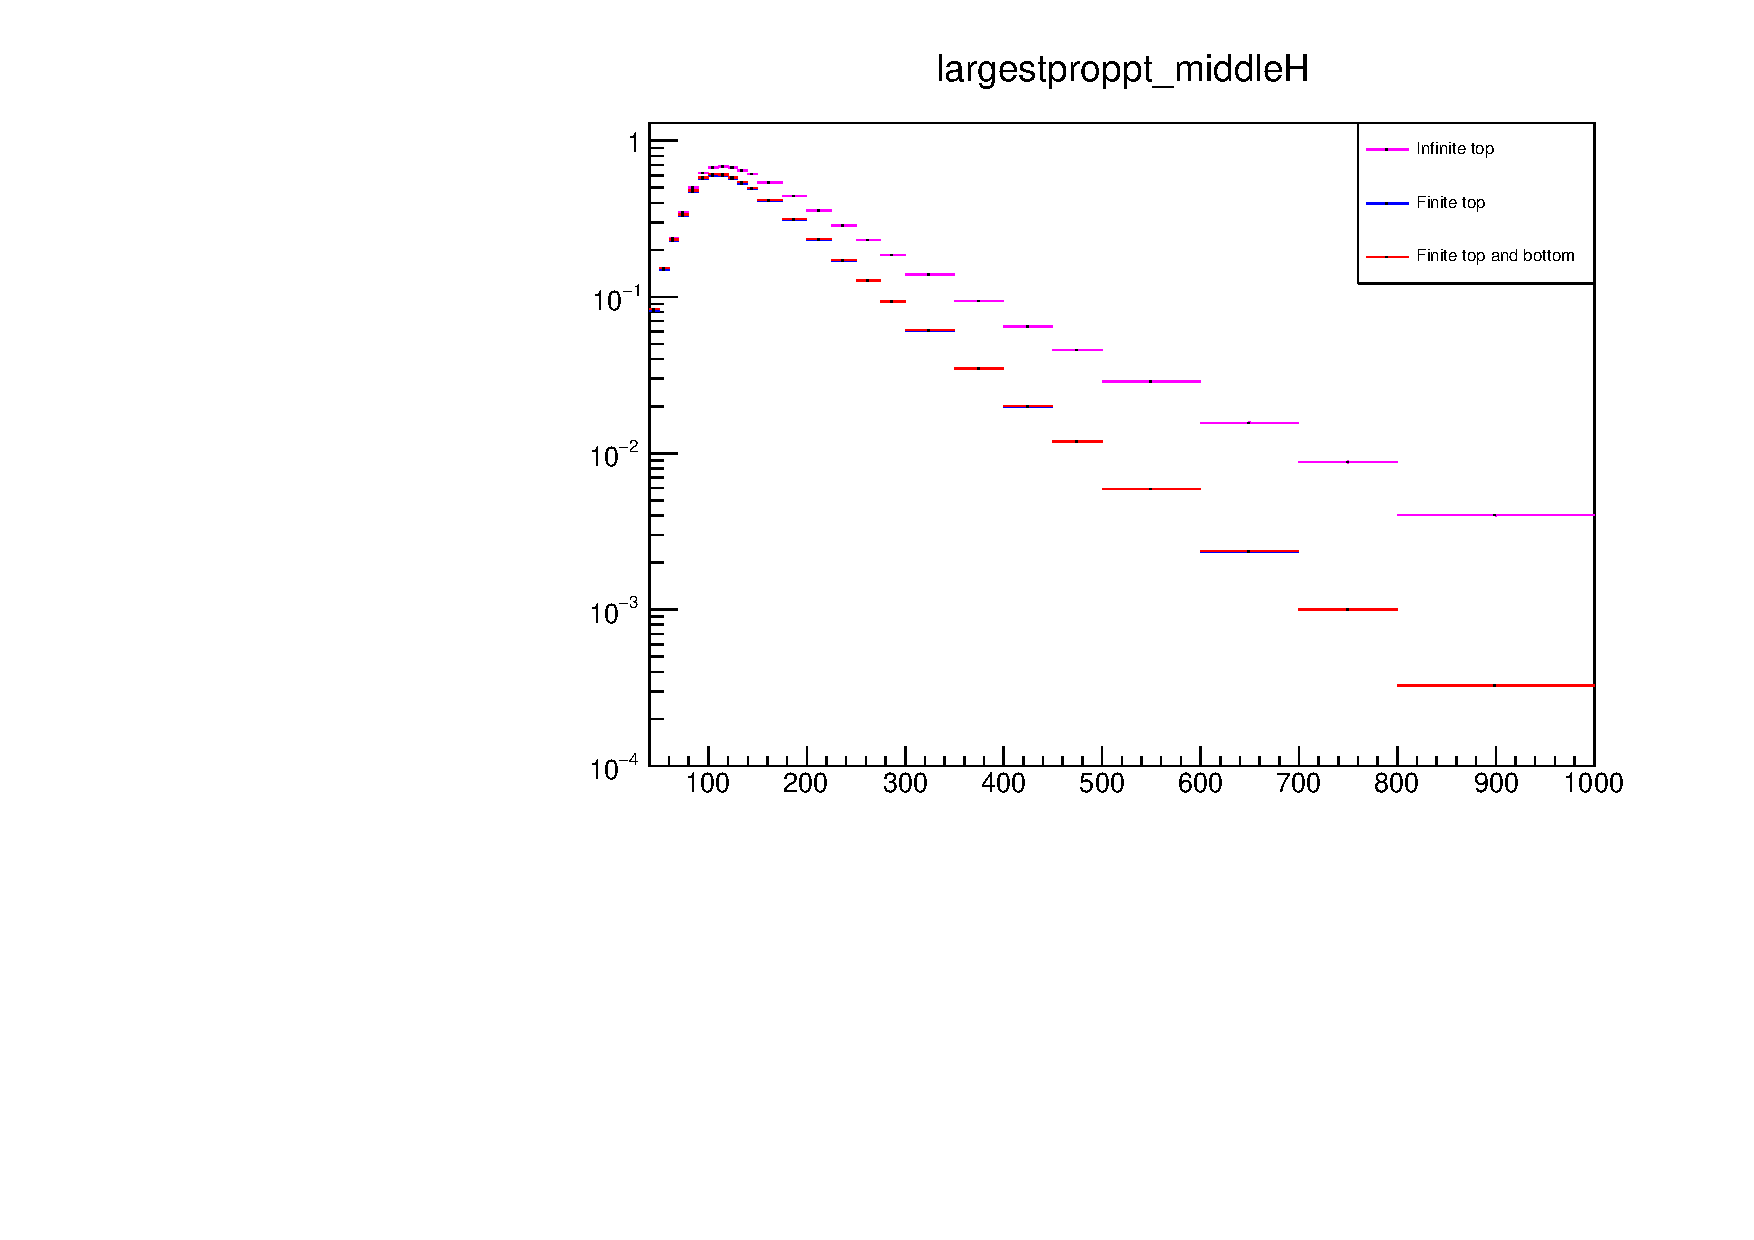
\includegraphics[scale=0.72]{Images/largestproppt.pdf}
\caption{Comparison of infinite top mass, finite top mass and finite top + bottom mass cross sections in $gg \to gggH$, binned in the maximum $p_T$ of a gluon entering into the Higgs vertex. }
\label{fig:maxprop}
\end{figure}

Unfortunately, there has so far not been many analyses of Higgs plus jets physics from the LHC and so we are not able to compare our new predictions against real data yet. We are, however, now in a prime position to provide predictions for any such data when it arrives. 


%\todo{Mention no compare with data because lack of it}